\documentclass[10pt]{article}

% Idioma y codificación
\usepackage[utf8]{inputenc}
\usepackage[spanish]{babel}

% Márgenes
\usepackage{geometry}
\geometry{top=2.5cm, bottom=2.5cm, left=2.5cm, right=2.5cm}

% Gráficos y Tablas
\usepackage{pdflscape}
\usepackage{graphicx}
\usepackage{amsmath}
\usepackage{pdfpages}
\usepackage{multicol}
\usepackage{float}
\usepackage[table]{xcolor} % UNA SOLA VEZ Y CON [table]
\usepackage{booktabs}
\usepackage{xltabular}
\usepackage{caption}
\usepackage{subcaption}
\usepackage{array}

% Listings para código
\usepackage{listings}
\lstdefinestyle{terminal}{
	backgroundcolor=\color{gray!10},
	basicstyle=\ttfamily\small,
	keywordstyle=\color{blue},
	commentstyle=\color{gray},
	frame=single,
	columns=fullflexible,
	morecomment=[l]{//}
}
\lstset{
	inputencoding=utf8,
	extendedchars=true,
	literate={á}{{\'a}}1 {é}{{\'e}}1 {í}{{\'i}}1 {ó}{{\'o}}1 {ú}{{\'u}}1 {ñ}{{\~n}}1
}

% Hipervínculos
\usepackage[hidelinks]{hyperref}
\hypersetup{
	colorlinks=true,
	linkcolor=blue,
	filecolor=magenta,
	urlcolor=cyan,
}

% Encabezados y pies de página
\usepackage{fancyhdr}
\pagestyle{fancy}
\fancyhf{}
\fancyfoot[R]{\thepage}

% Formato de títulos
\usepackage{titlesec}
\titleformat{\subsection}{\normalfont\large\bfseries}{\thesubsection}{1em}{}
\titleformat{\subsubsection}{\normalfont\normalsize\bfseries}{\thesubsubsection}{1em}{}

% Datos de la portada
\title{\textit{CARD PARTNER}\\ Una web para amantes de los \textit{TCGS}}

\author{
	\textbf{\small ÁLVAREZ FULCONIS, MARCOS PALATINO}\\
	\textbf{\small LÓPEZ PRIMO, ÁLVARO}\\
	\textbf{\small OTERO GARCÍA, SERGIO}\\
	\textbf{\small SANTIESTEBAN MENDO, EDGAR}
}

\date{Curso 25-26}

\begin{document}
	
	\begin{titlepage}
		\centering
		% Asegúrate de que la ruta al PDF de la UVA sea correcta
		%
\includegraphics[scale=0.3]{./Recursos/UVA-3881270087.pdf}\\[0.5cm] 
		\rule{\linewidth}{0.2mm}\\[0.4cm]
		{\huge\bfseries CARD PARTNER\par}
		{\large Una web para amantes de los TCGS\par}
		\rule{\linewidth}{0.2mm}\\[1.5cm]
		{\Large\bfseries Servicios y Sistemas Web}\\[0.3cm]
		{\large\bfseries Laboratorio L2 \\ GRUPO 33}\\[1cm]
		{\Large \begin{tabular}{c} ÁLVAREZ FULCONIS, MARCOS \\ LÓPEZ PRIMO, ÁLVARO \\ OTERO GARCÍA, SERGIO \\ SANTIESTEBAN MENDO, EDGAR \end{tabular}}\\[1.5cm]
		{\Large Curso 25-26}
	\end{titlepage}
	
	\pagenumbering{gobble}
	\tableofcontents \newpage
	
	\pagenumbering{arabic} 
	\setcounter{page}{1}
	
	\section{Presentación del equipo}
        El desarrollo de \textit{Card Partner} ha sido realizado por el Grupo 33, formado por Marcos Álvarez Fulconis, Álvaro López Primo, Sergio Otero García y Edgar Santiesteban Mendo. A lo largo de las distintas fases del proyecto, hemos ido adaptando nuestra forma de trabajo según las necesidades de cada entrega.\\
        
        En la primera fase del proyecto, centramos el trabajo en definir la idea inicial, estudiar el problema que queríamos resolver, analizar los usuarios objetivo y plantear los primeros bocetos de la aplicación. Esta fase nos permitió establecer la base conceptual de \textit{Card Partner} como una plataforma orientada a jugadores de TCG, tomando como referencia inicial el \textit{TCG de One Piece}.\\
        
        En la segunda fase, hicimos evolucionar el trabajo hacia una definición más formal del sistema. Desarrollamos los requisitos funcionales y no funcionales, el modelo de dominio, el mapa del sitio web y los principales flujos de navegación. Esta etapa nos sirvió para transformar la idea inicial en una propuesta más estructurada, identificando las entidades principales del sistema, las relaciones entre ellas y las vistas necesarias para cubrir las funcionalidades previstas.\\
        
        Finalmente, en la tercera fase, hemos reorganizado el equipo en dos bloques principales de trabajo: frontend y backend. Esta división nos ha permitido optimizar el desarrollo, reducir conflictos en el repositorio y aprovechar mejor las capacidades de cada integrante. El equipo de frontend se ha centrado en la construcción de las vistas JSP, la navegación y el diseño visual mediante CSS. Por otro lado, el equipo de backend se ha encargado de la base de datos, los modelos, los DAOs, los Servlets y la integración de la lógica de la aplicación.
        
    \subsection{Organización del trabajo}
        Para esta última fase del proyecto, hemos decidido dividir el desarrollo en dos áreas principales. La primera corresponde al frontend, encargado de la parte visual y de la interacción con el usuario. La segunda corresponde al backend y a la gestión de datos, encargada de la persistencia, la conexión con la base de datos y la lógica principal de la aplicación.\\
        
        Hemos elegido esta organización por varios motivos. En primer lugar, nos ha permitido trabajar de forma paralela sobre partes diferenciadas del sistema. En segundo lugar, ha reducido los conflictos al utilizar Git, ya que cada grupo ha trabajado principalmente sobre carpetas y archivos distintos. Por último, nos ha permitido que cada integrante se especialice en aquellas tareas en las que podía aportar mayor valor al proyecto.\\
        
        El equipo de frontend se ha encargado principalmente de la maquetación, el diseño visual, la navegación entre vistas y la implementación de las páginas JSP. Dentro de este bloque se han desarrollado vistas como la página principal, el catálogo de cartas, la visualización de cartas, las páginas de mazos, el constructor de mazos, el perfil de usuario, el login, el registro y las secciones de contenido social.\\
        
        El equipo de backend y gestión se ha centrado en el diseño e implementación de la base de datos, la creación de los scripts SQL, la definición de las clases del modelo, la construcción de los DAOs, la implementación de los Servlets y la automatización de la creación de la base de datos en local. También se ha encargado de transformar los datos necesarios para poblar la aplicación y de preparar la conexión entre la capa de presentación y la capa de persistencia.
        
    \subsection{Reparto de carga de trabajo} 
        Aunque todos los integrantes hemos participado en la revisión general del proyecto y en la toma de decisiones principales, cada miembro ha tenido una responsabilidad predominante. La distribución final del trabajo se resume en la siguiente tabla:
        
        \begin{table}[H]
            \centering
            \renewcommand{\arraystretch}{1.3}
            \begin{tabular}{|>{\centering\arraybackslash}p{4cm}|>{\centering\arraybackslash}p{2cm}|p{8cm}|}
            \hline
            \textbf{Nombre} & \textbf{Porcentaje} & \textbf{Responsabilidad principal} \\
            \hline
            \multicolumn{3}{|c|}{\textbf{Equipo Frontend}} \\
             \hline
                Marcos Álvarez Fulconis & 25\% & Desarrollo de vistas relacionadas con cartas y apartado social, apoyo en la navegabilidad general de la aplicación, revisión visual de las páginas y maquetación del documento. \\
            \hline
                Sergio Otero García & 25\% & Desarrollo de vistas relacionadas con mazos, login, registro, página principal y constructor de mazos. Apoyo en la redacción del documento y en la integración visual de las distintas secciones. \\
                \hline
            \multicolumn{3}{|c|}{\textbf{Equipo Backend y Gestión de Datos}} \\
            \hline
                Álvaro López Primo & 25\% & Creación del esquema de la base de datos, colaboración en el modelo entidad-relación, población de la base de datos, transformación de datos externos y automatización de scripts para MariaDB en local. Apoyo en la redacción técnica del documento. \\
            \hline
                Edgar Santiesteban Mendo & 25\% & Colaboración en el modelo entidad-relación, creación de esquemas de base de datos, desarrollo de clases del modelo, DAOs y DTOs, y apoyo en la redacción técnica del documento. \\
            \hline
            \end{tabular}
            \caption{Distribución de responsabilidades por miembro}
        \end{table}
        
    \subsection{Justificación de la organización}
        Hemos considerado que la división del trabajo en frontend y backend era adecuada para el tipo de aplicación desarrollada. \textit{Card Partner} requiere una interfaz visual amplia, con múltiples vistas para cartas, mazos, perfil, noticias, guías y torneos, pero también necesita una base de datos consistente y una lógica de servidor capaz de gestionar usuarios, cartas, mazos, comentarios, valoraciones y contenido editable.\\
        
        Por ello, separar las responsabilidades nos ha permitido avanzar de forma más ordenada. El equipo de frontend ha podido centrarse en mantener una apariencia homogénea en toda la aplicación, reutilizando elementos comunes como la cabecera, el menú de navegación, las tarjetas de cartas y mazos, y los estilos generales. Al mismo tiempo, el equipo de backend ha podido centrarse en definir correctamente las entidades, relaciones, scripts SQL y mecanismos de acceso a datos.\\
        
        Esta metodología también nos ha facilitado la corrección de errores detectados en entregas anteriores. Por ejemplo, hemos incorporado una vista de perfil de usuario más completa, hemos desarrollado mejor la distinción entre mazos de comunidad y mazos meta, y hemos consolidado la existencia de usuarios con distintos roles dentro del sistema. Además, la creación de scripts de automatización para la base de datos nos ha permitido que todos los miembros puedan trabajar con una estructura local equivalente, evitando problemas derivados de no disponer de un servidor remoto común.


    %-------------------------------- COMPROBAR SI SOBRA ESTA PARTE POR REPETICION ------------------------%
        
    % \subsection{Evolución del trabajo respecto a entregas anteriores}
    %     El proyecto ha evolucionado de manera progresiva. En la primera entrega trabajamos principalmente sobre la idea inicial, el análisis del problema y los primeros bocetos. En la segunda entrega formalizamos el sistema mediante requisitos, modelo de dominio y mapa de navegación. En la tercera entrega avanzamos hacia una implementación funcional, incorporando JSP, CSS, Servlets, DAOs, clases de dominio y scripts SQL.\\
        
    %     Esta evolución nos ha permitido transformar \textit{Card Partner} de una propuesta conceptual a una aplicación web con una estructura técnica más completa. El resultado final mantiene la idea inicial de centralizar herramientas útiles para jugadores de TCG, pero incorpora una arquitectura más definida, una base de datos relacional, una separación clara entre vistas y lógica de servidor, y una organización más precisa de los distintos módulos de la plataforma.
		
    \section{Introducción: descripción del sistema web}
        
    \subsection{Contexto y problema abordado}        
        El mundo de los TCG, o Trading Card Games, ha crecido notablemente en los últimos años y cada vez reúne a más jugadores con perfiles muy distintos. Algunos usuarios se acercan por primera vez al juego y necesitan aprender sus reglas básicas, mientras que otros ya conocen las mecánicas y buscan herramientas para consultar mazos competitivos, estudiar cartas, revisar precios o compartir sus propias construcciones con la comunidad.\\
        
        Uno de los principales problemas que hemos detectado es la dispersión de la información. Actualmente, los jugadores suelen utilizar distintas páginas para consultar precios, buscar cartas, revisar mazos de torneos, aprender reglas o seguir las novedades del juego. Esto obliga al usuario a cambiar constantemente de plataforma según la tarea que quiera realizar, lo que dificulta especialmente la experiencia de los jugadores novatos.\\
        
        Por este motivo, hemos decidido plantear \textit{Card Partner} como una aplicación web centralizada para jugadores y aficionados a los TCG, eligiendo como referencia inicial el \textit{\textbf{One Pice TCG}}, de tal forma que podamos acotar el alcance del proyecto y trabajar con un dominio concreto, pudiendo amplicar la estructura a futuro para poder añadir otros juegos de cartas coleccionables. Aunque existen páginas especializadas en aspectos concretos, nuestra propuesta busca reunir en una misma plataforma las funcionalidades más habituales: consulta de cartas, visualización de precios, creación y gestión de mazos, consulta de mazos meta, publicación de mazos de la comunidad, noticias, guías, torneos y funcionalidades sociales como comentarios, valoraciones y mazos guardados.
        
    \subsection{Análisis de soluciones existentes}        
        Antes de definir nuestra solución, hemos analizado varias plataformas utilizadas actualmente por la comunidad. Cada una de ellas resuelve una parte del problema, pero ninguna centraliza todas las necesidades que hemos identificado en una única experiencia.
        
        \begin{table}[H]
            \centering
            \renewcommand{\arraystretch}{1.3}
            \begin{tabular}{|p{3.2cm}|p{5.2cm}|p{5.2cm}|}
                \hline
                \textbf{Plataforma} & \textbf{Fortalezas} & \textbf{Limitaciones detectadas} \\
                \hline
                    \href{https://www.cardmarket.com/es/OnePiece}{\textit{Card Market}} & Es una de las plataformas más completas para consultar precios y realizar compraventa de cartas de distintos TCG. & Está orientada principalmente al mercado de cartas, por lo que no ofrece una experiencia centrada en la creación de mazos, el aprendizaje del juego o la interacción entre usuarios. \\
                \hline
                    \href{https://deckbuilder.egmanevents.com/optcg/cards}{\textit{EggmanEvents}} & Permite consultar mazos utilizados en torneos y resulta útil para jugadores interesados en el entorno competitivo. & Su enfoque está muy ligado a resultados competitivos. Además, puede resultar menos intuitiva para usuarios novatos y no está orientada a que el usuario cree, gestione y comparta sus propios mazos. \\
                \hline
                    \href{https://en.onepiece-cardgame.com/beginners/}{\textit{One Piece Card Game}} & Es la fuente más fiable para consultar productos oficiales, reglas básicas y materiales introductorios del juego. & No funciona como comunidad de usuarios ni ofrece herramientas completas para construir mazos, valorar listas, guardar contenido personalizado o consultar precios de mercado. \\
                \hline
                
                    \href{https://onepiece.limitlesstcg.com}{\textit{One Piece Limitless}} & Reúne información competitiva, estadísticas de torneos, cartas y herramientas relacionadas con el juego. & Aunque ofrece información útil para jugadores avanzados, no centraliza en una misma experiencia el aprendizaje para principiantes, la gestión personal de mazos, los precios y la interacción social. \\
                \hline
            \end{tabular}
            \caption{Comparación de plataformas existentes relacionadas con One Piece TCG}
        \end{table}

    \newpage
        
        A partir de este análisis, hemos observado que la principal oportunidad de mejora no consiste en crear una herramienta completamente aislada de las ya existentes, sino en reunir en un mismo entorno varias funcionalidades que actualmente se encuentran repartidas. De esta forma, \textit{Card Partner} busca reducir la fragmentación de la experiencia del usuario y ofrecer una navegación más directa entre cartas, mazos, contenido informativo y comunidad.
        
    \subsection{Solución propuesta}        
        \textit{Card Partner} se plantea como una aplicación web para centralizar las tareas habituales de los jugadores de TCG. La aplicación permite consultar un catálogo de cartas, acceder al detalle de cada una, revisar información como tipo, color, coste, poder o precio, y utilizar estas cartas como base para la creación de mazos. Además, hemos incorporado un módulo de mazos que diferencia entre mazos de la comunidad y mazos meta:
        
        \begin{itemize}
            \item Los \textbf{mazos de la comunidad} representan listas creadas y compartidas por usuarios.
            \item Los \textbf{mazos meta} permiten destacar construcciones competitivas o recomendadas por sus resultados.
        \end{itemize}
        
        Esta separación permite que la aplicación sea útil tanto para jugadores que buscan \textit{inspiración competitiva} como para usuarios que quieren compartir sus propias ideas.\\
        
        También hemos incluido una parte social y editorial. Por un lado, los usuarios pueden comentar, valorar y guardar mazos. Por otro lado, la aplicación cuenta con secciones de noticias, guías y torneos, pensadas para mantener al usuario informado y facilitar la entrada de jugadores principiantes al TCG.\\
        
        Por último, hemos definido una parte de usuario que permite registrar cuentas, iniciar sesión, gestionar el perfil y acceder a funcionalidades personalizadas. Esta parte es importante porque diferencia la experiencia de un visitante no registrado de la de un jugador registrado, que puede crear, guardar y gestionar contenido propio.

	\newpage

    \subsection{Borrador de solución}
	Para tener un visión más clara del diseño del \textit{frontend} de nuestra web hemos realizado dos fases de bocetaje:
	\subsubsection{Primera versión del bocetaje}
	En la primera fase hemos realizado unos esquemas a mano alzada sobre el aspecto y funcionalidades de la web (para consultar los bocetos con más detalle puesto que \underline{no} son imágenes vectorizadas diríjase a \href{https://uvaes-my.sharepoint.com/:b:/g/personal/alvaro_lopez_primo_estudiantes_uva_es/IQDlwgU7uvVIR4IvbixZFawhAXxjL6flgH43ePd4Q4bNtks?e=ghkMdm}{este enlace}).
	\begin{figure}[H]
		\centering
		\begin{subfigure}{0.45\textwidth}
			\centering
			\includegraphics[width=\textwidth]{Recursos/inicio.png}
			\caption{Vista inicial de la página con la opción de \textit{login} y con una cuenta ya creada donde se verán unas breves noticias sobre el \textit{TCG}, un apartado de las normas básicas del juego y una sección de mazos recomendados para principiantes.}
			\label{InicioPagina}
		\end{subfigure}
		\hfill 
		\begin{subfigure}{0.45\textwidth}
			\centering
			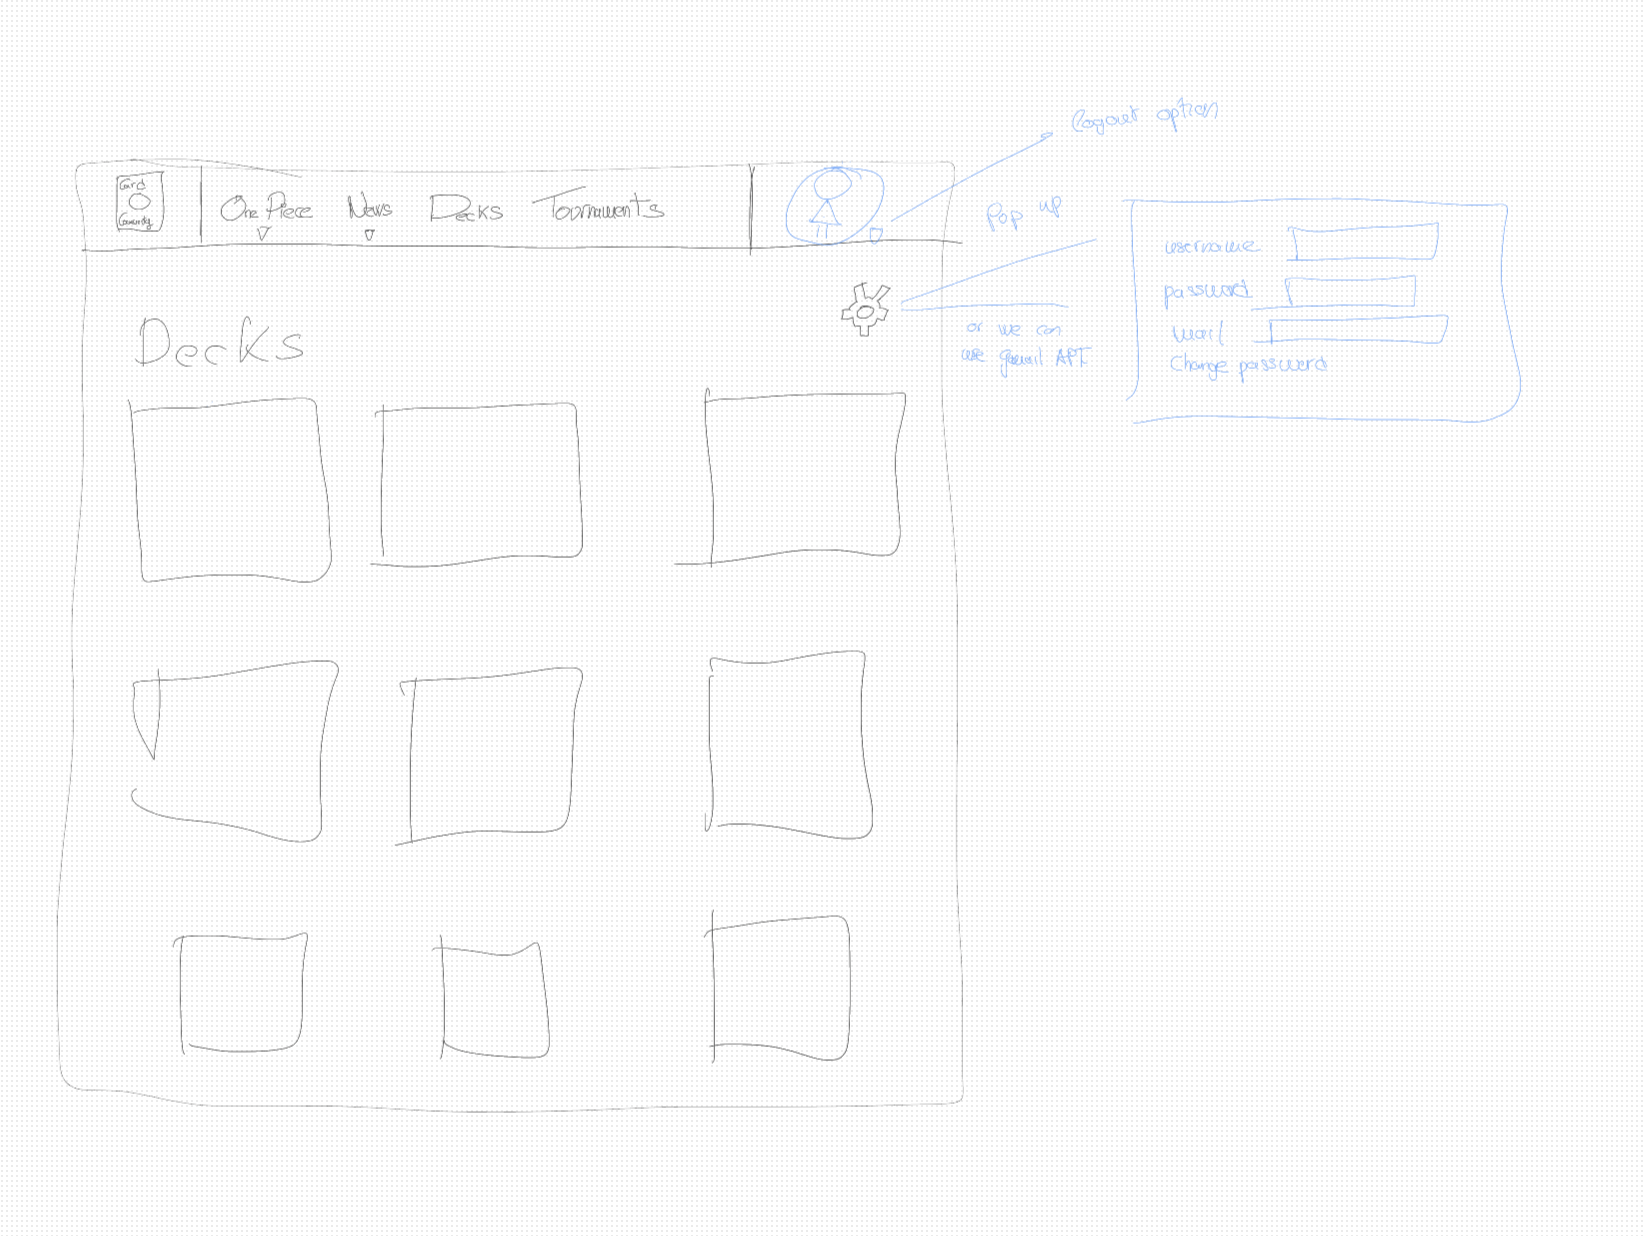
\includegraphics[width=\textwidth]{Recursos/user.png}
			\caption{Vista del usuario donde podrá ver los mazos que ha creado y una rueda de opción donde poder realizar diferentes funciones sobre su perfil (cambiar contraseña)}
			\label{UserView}
		\end{subfigure}
	\end{figure}
	\begin{figure}[H]
		\centering
		\begin{subfigure}{0.45\textwidth}
			\centering
			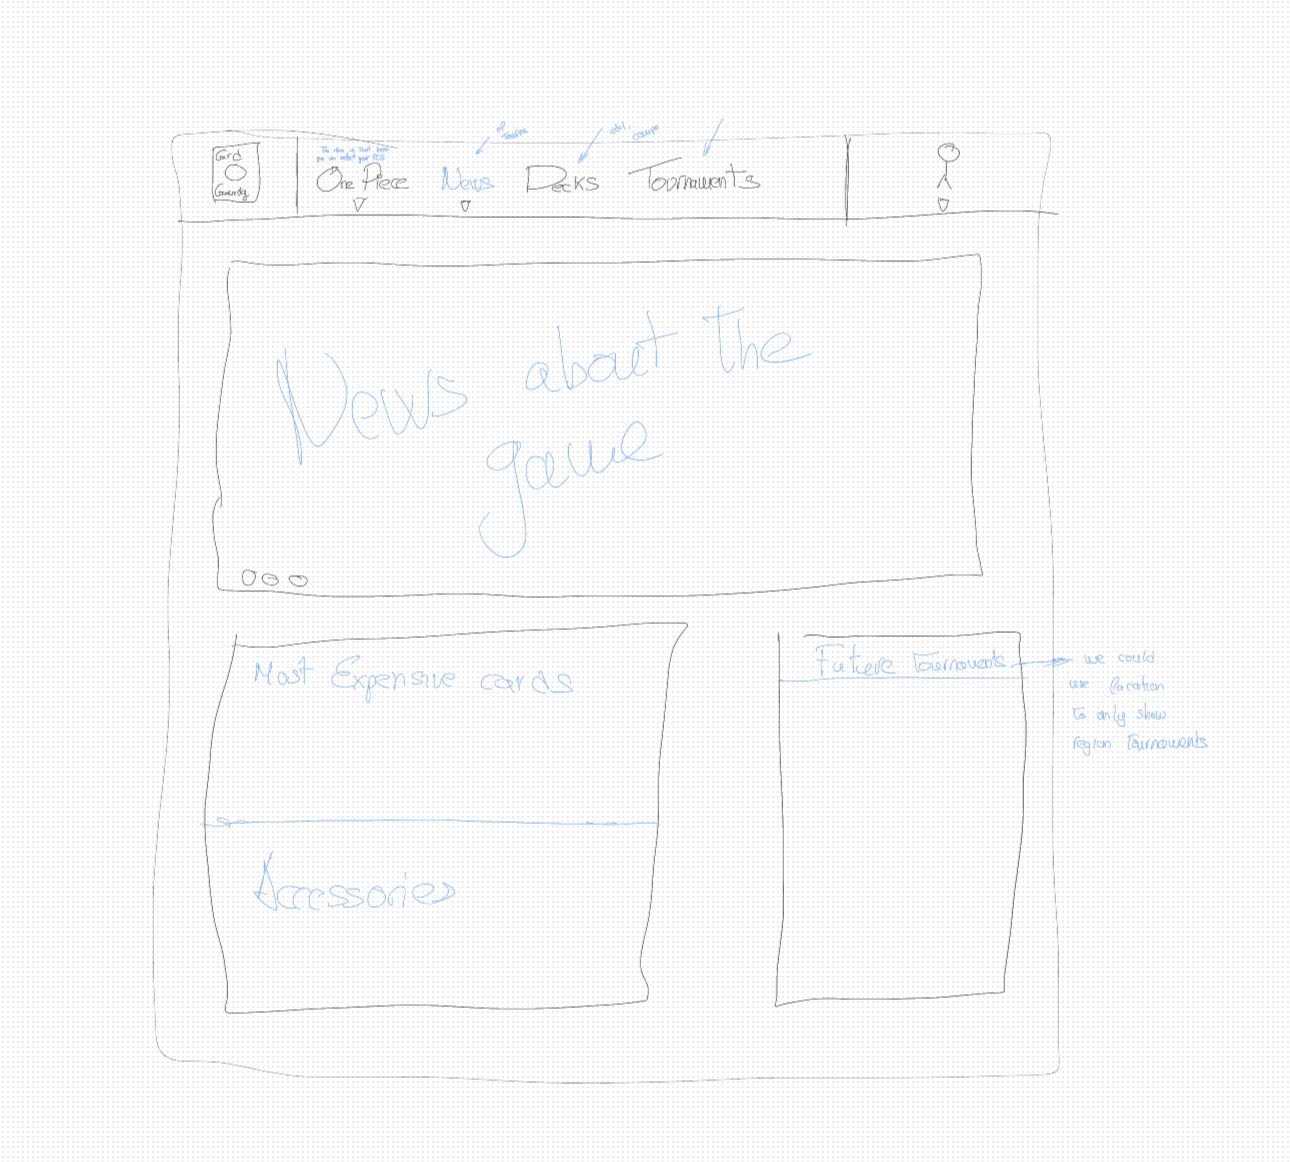
\includegraphics[width=\textwidth]{Recursos/noticias.png}
			\caption{Vista del apartado de noticias. En ella observamos novedades del \textit{TCG} así como una selección de cartas más caras y de accesorios típicos para dichos juegos así como una lista de los futuros torneos.}
			\label{Noticias}
		\end{subfigure}
		\hfill 
		\begin{subfigure}{0.45\textwidth}
			\centering
			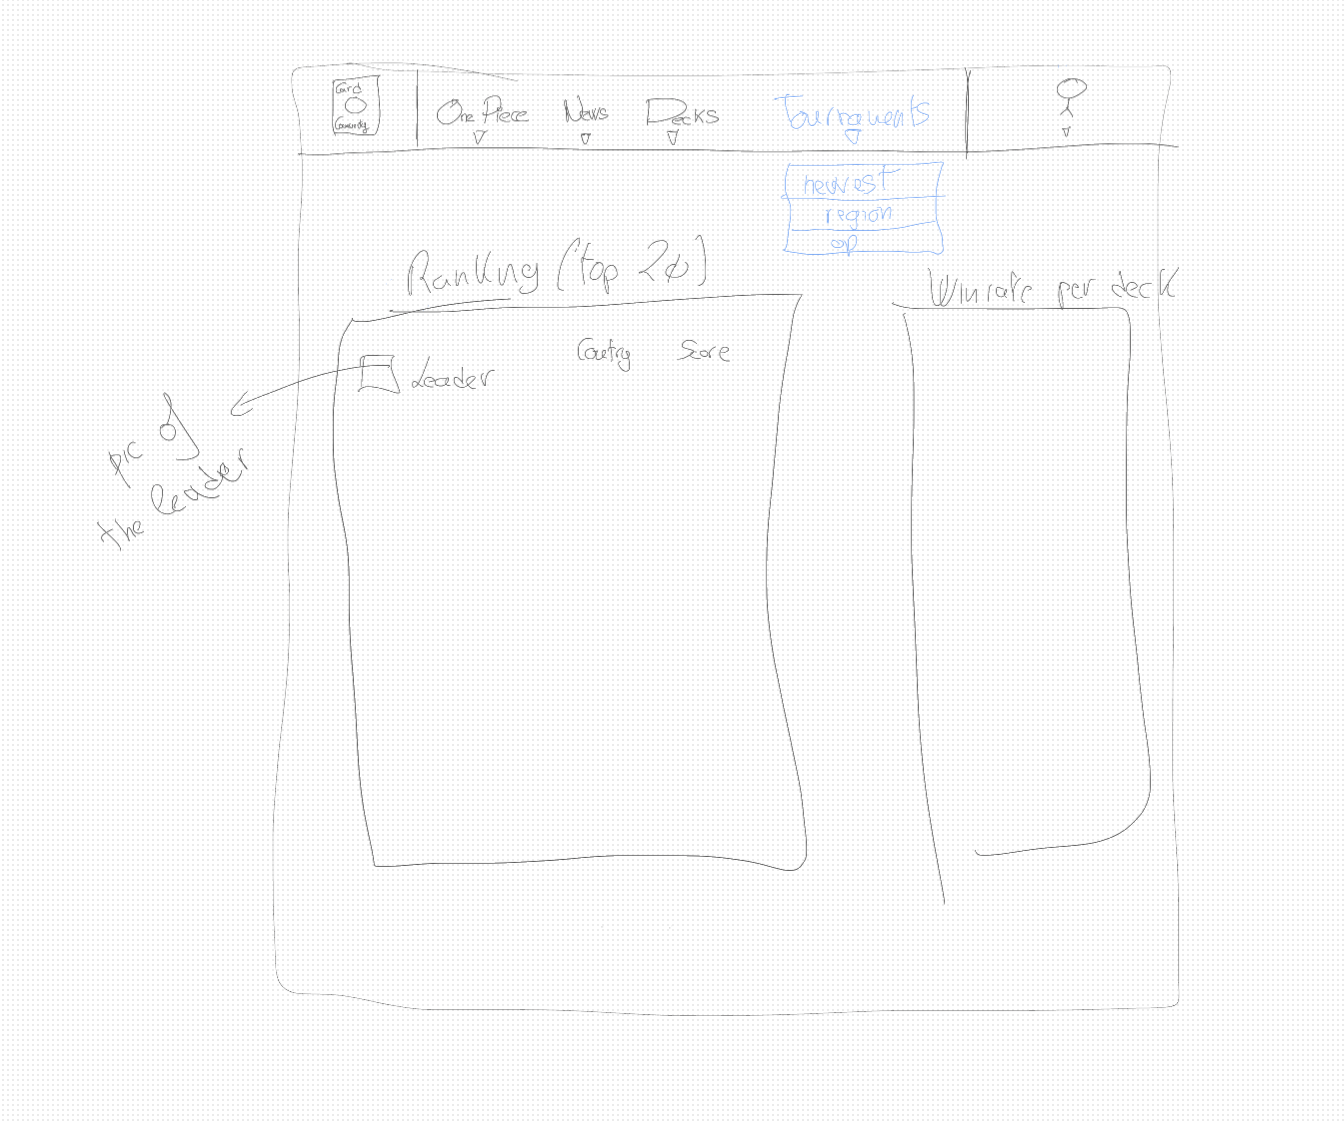
\includegraphics[width=\textwidth]{Recursos/tournaments.png}
			\caption{Vista de la pestaña de torneos. Incluye un ranking global de mazos y un porcentaje de victoria de cada líder.}
			\label{fig:imagen_der}
		\end{subfigure}
	\end{figure}
	\begin{figure}[H]
			\centering
			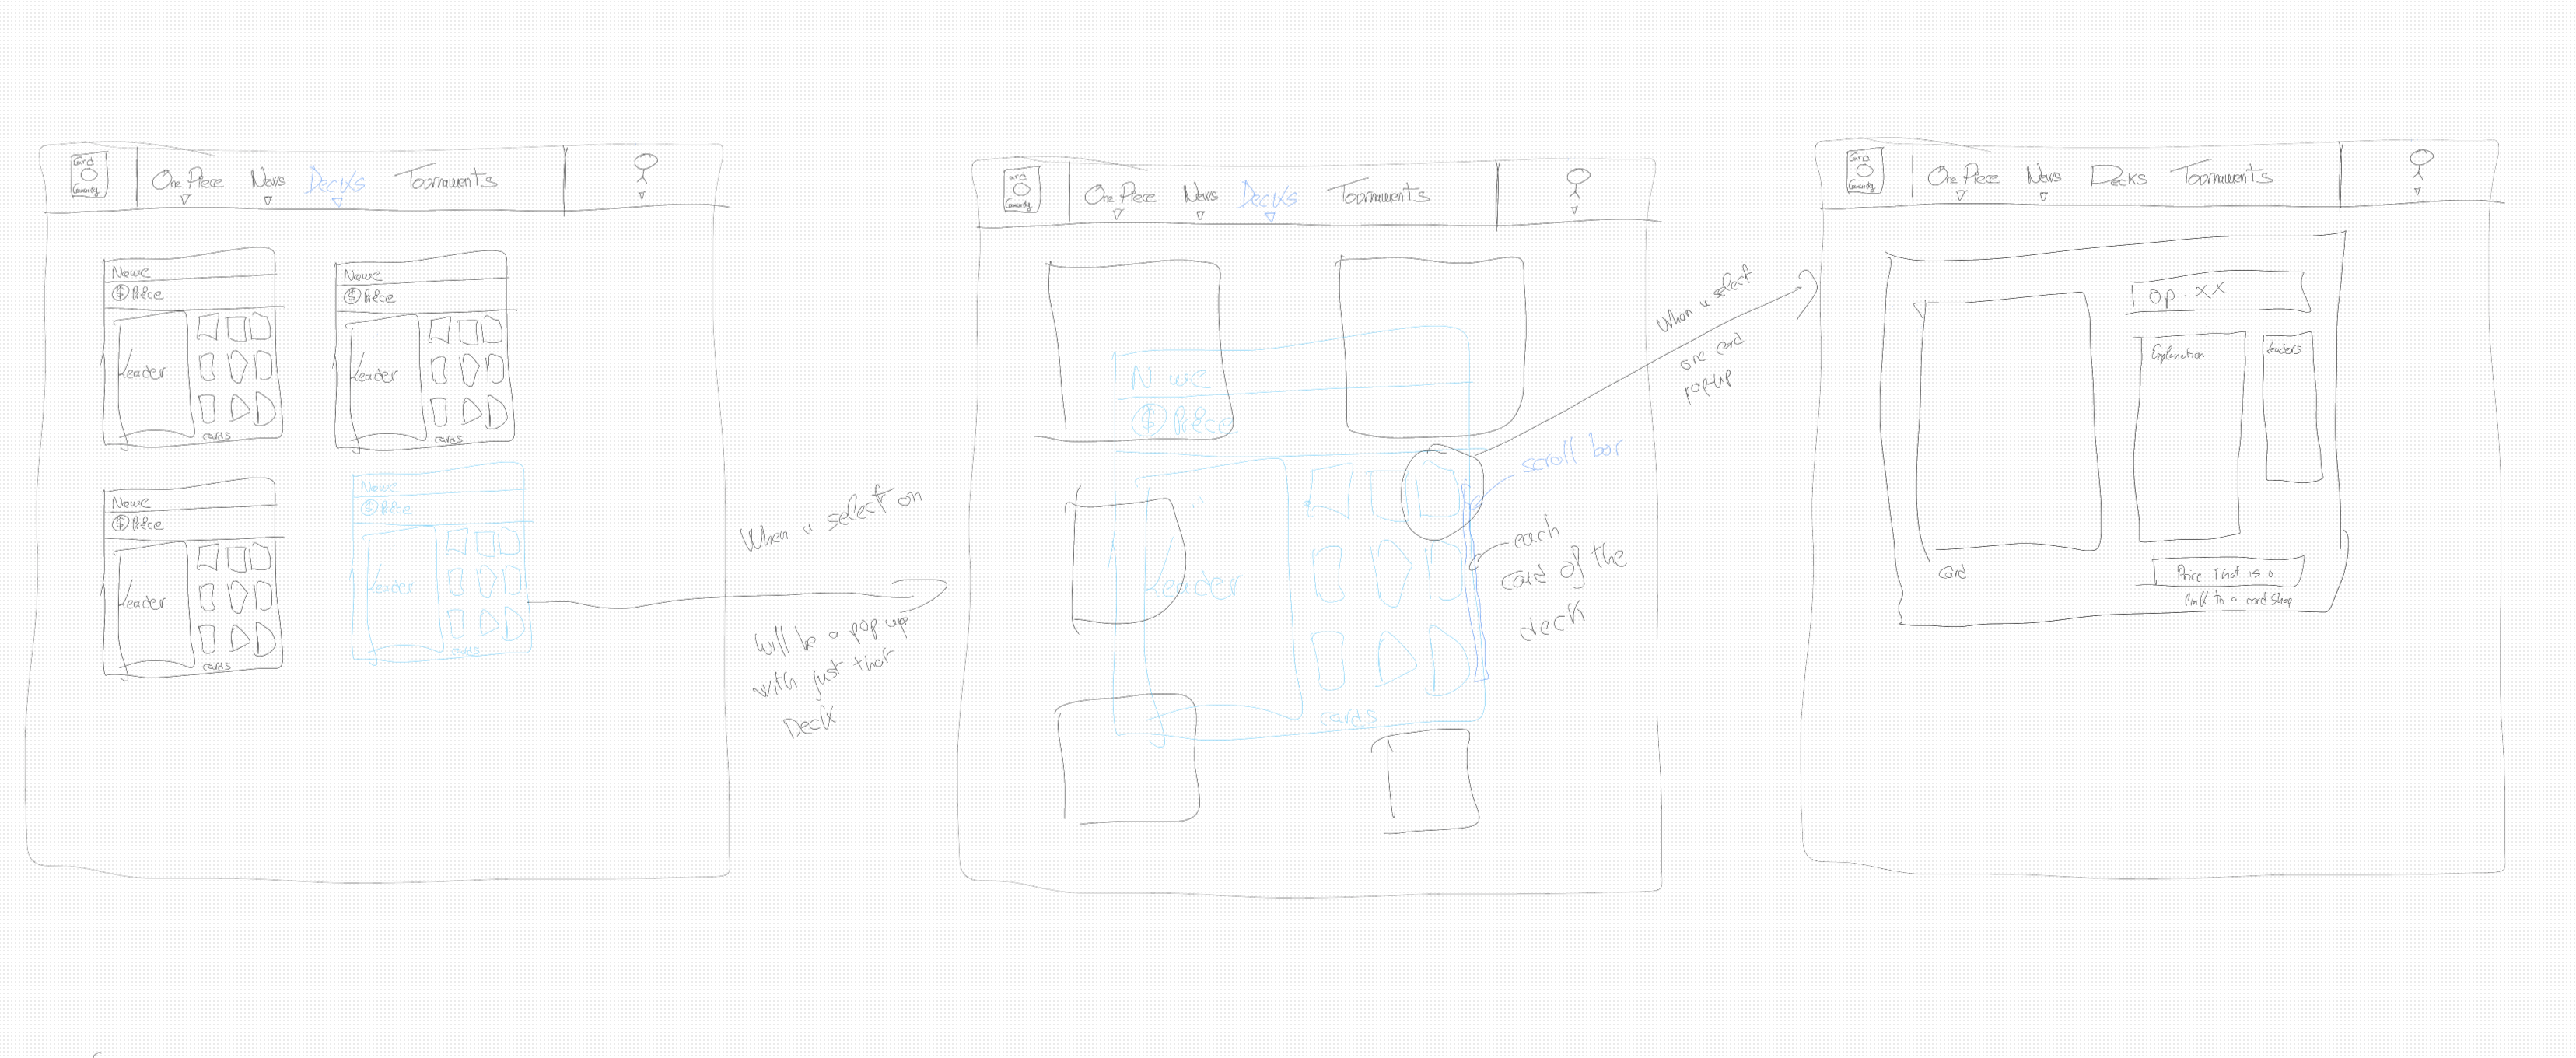
\includegraphics[width=0.85\textwidth]{Recursos/decks.png}
			\caption{Vista del apartado Deck. Se muestran los diferentes mazos creados por la comunidad, con la opción de seleccionar sobre ellos y poder consultar todas las cartas. Además se incluye una opción a las personas con una cuenta en la web de comentar en los mazos}
	\end{figure}
	
	
	\subsubsection{Segunda versión del bocetaje}
	Una vez que el grupo ha dado el visto bueno, decidimos emplear la herramienta draw.io para realizar  bocetos más limpios y organizados (para consultar los bocetos con más detalle, diríjase a \href{https://drive.google.com/file/d/1g8FwPydQRjYX_IET-vt37nWVM2JCpji7/view}{este enlace}). 
	
	Para la implementación de todas las funcionalidades explicadas anteriormente, hemos optado por organizarlas en diferentes apartados:
	\begin{itemize}
		\item \textbf{Comunidad:}
		\begin{itemize}
			\item Guías
			\item Noticias
			\item Torneos
		\end{itemize}
		
		\item \textbf{Mazos:}
		\begin{itemize}
			\item Meta y estadísticas
			\item Mazos de la comunidad (incluye filtros de búsqueda, valoraciones y comentarios)
			\item Creador de mazos
		\end{itemize}
		
		\item \textbf{Cartas:}
		\begin{itemize}
			\item Listado de cartas (incluye filtros de búsqueda, precio, estadísticas)
		\end{itemize}
		
		\item \textbf{Usuario:}
		\begin{itemize}
			\item Iniciar sesión/Crear cuenta
			\item Información personal de la cuenta (correo, contraseña, etc.)
			\item Mazos creados
			\item Mazos publicados
			\item Mazos guardados
			\item Interacciones del usuario (comentarios/valoraciones)
		\end{itemize}
	\end{itemize} 
	%\newpage
    A continuación añadimos imágenes que incluyen las diferentes vistas planteadas:
    \begin{landscape}
    	\thispagestyle{empty} 
    	\begin{figure}[p]
    		\centering
    		% El truco está en esta línea:
    		\makebox[\linewidth][c]{%
    			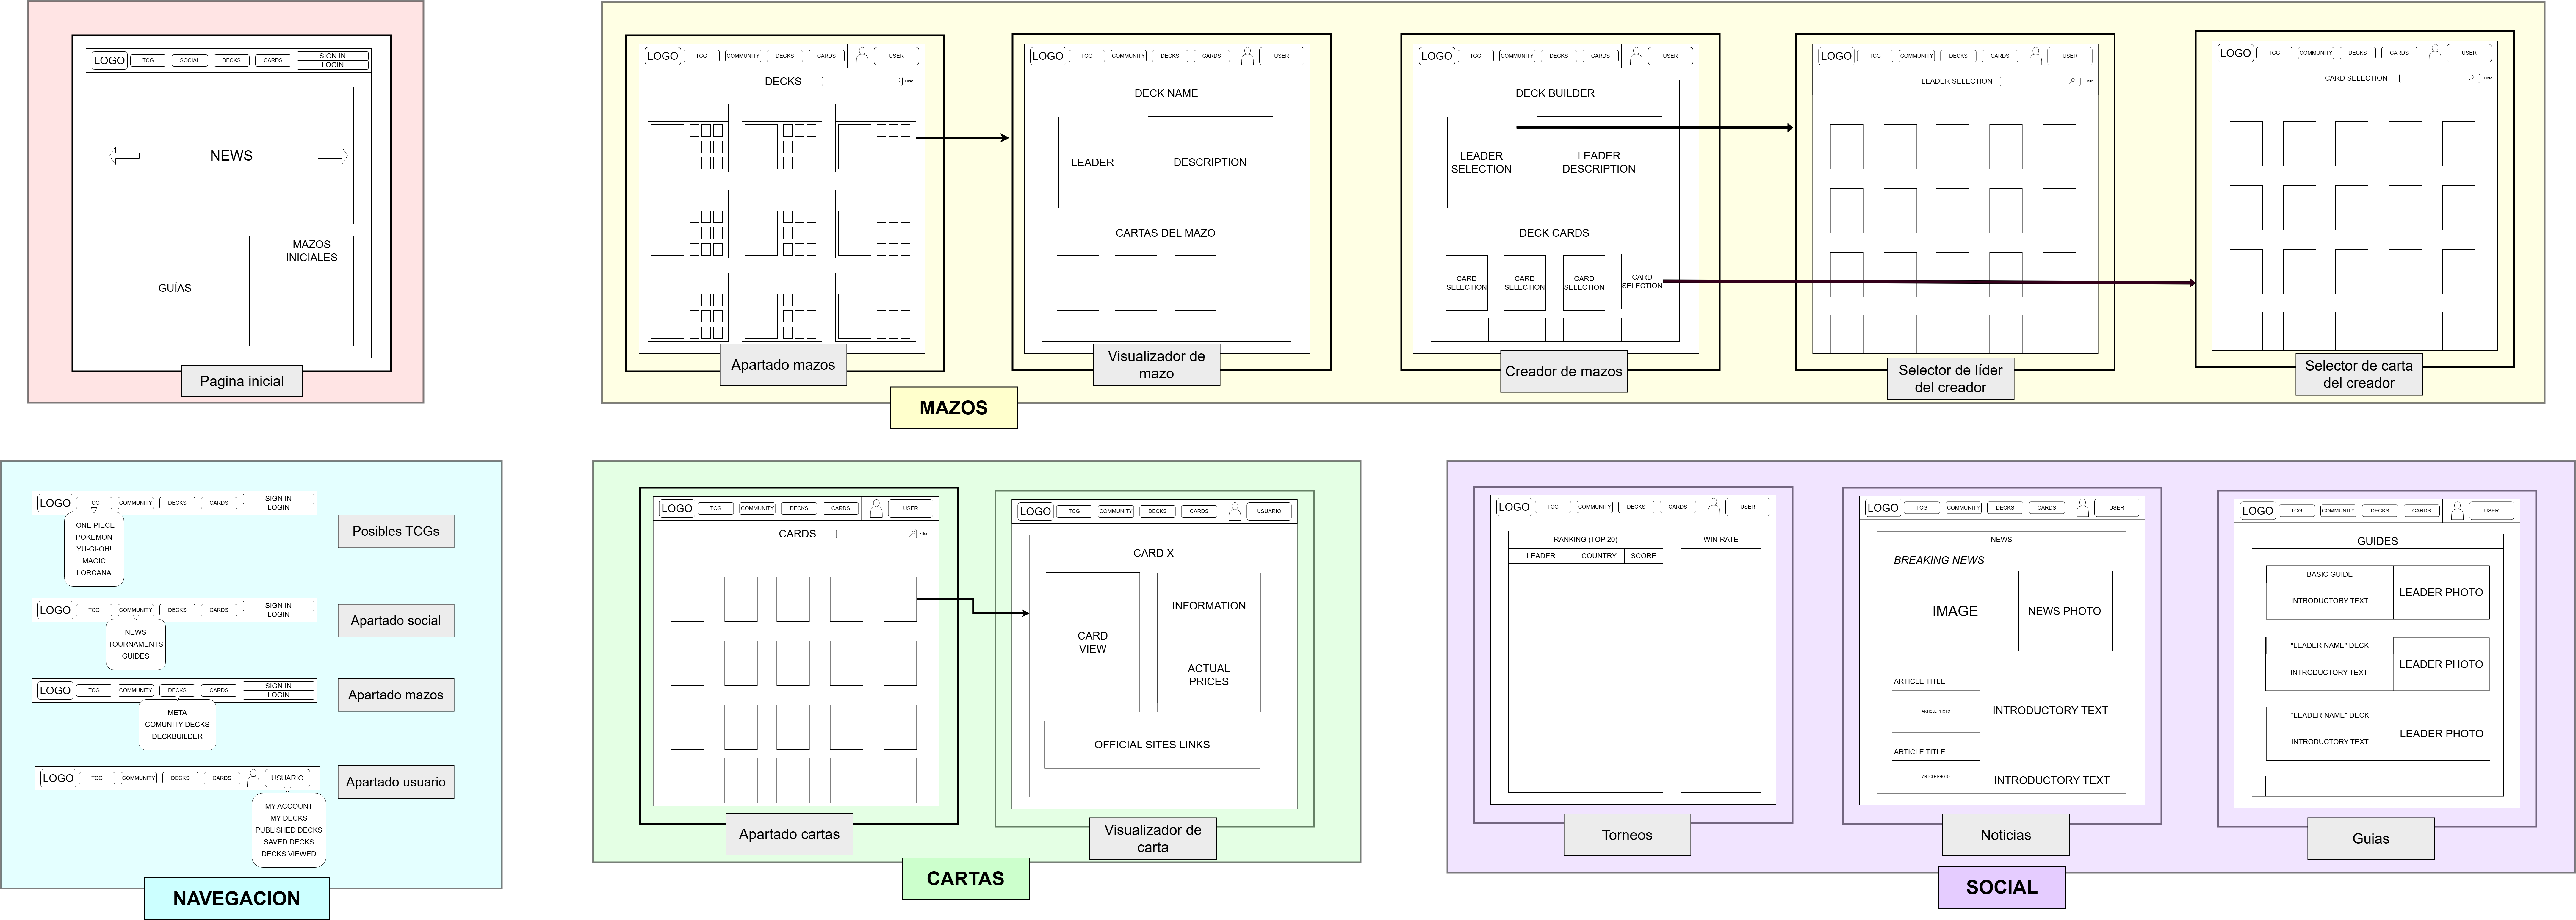
\includegraphics[width=1.18\linewidth, height=1.18\textheight, keepaspectratio]{Recursos/Bocetos2v2.png}
    		}
    		\caption{Vista completa de los bocetos de Draw.io}
    	\end{figure}
    \end{landscape}
    
	%\begin{figure}[H]
	%	\centering
	%	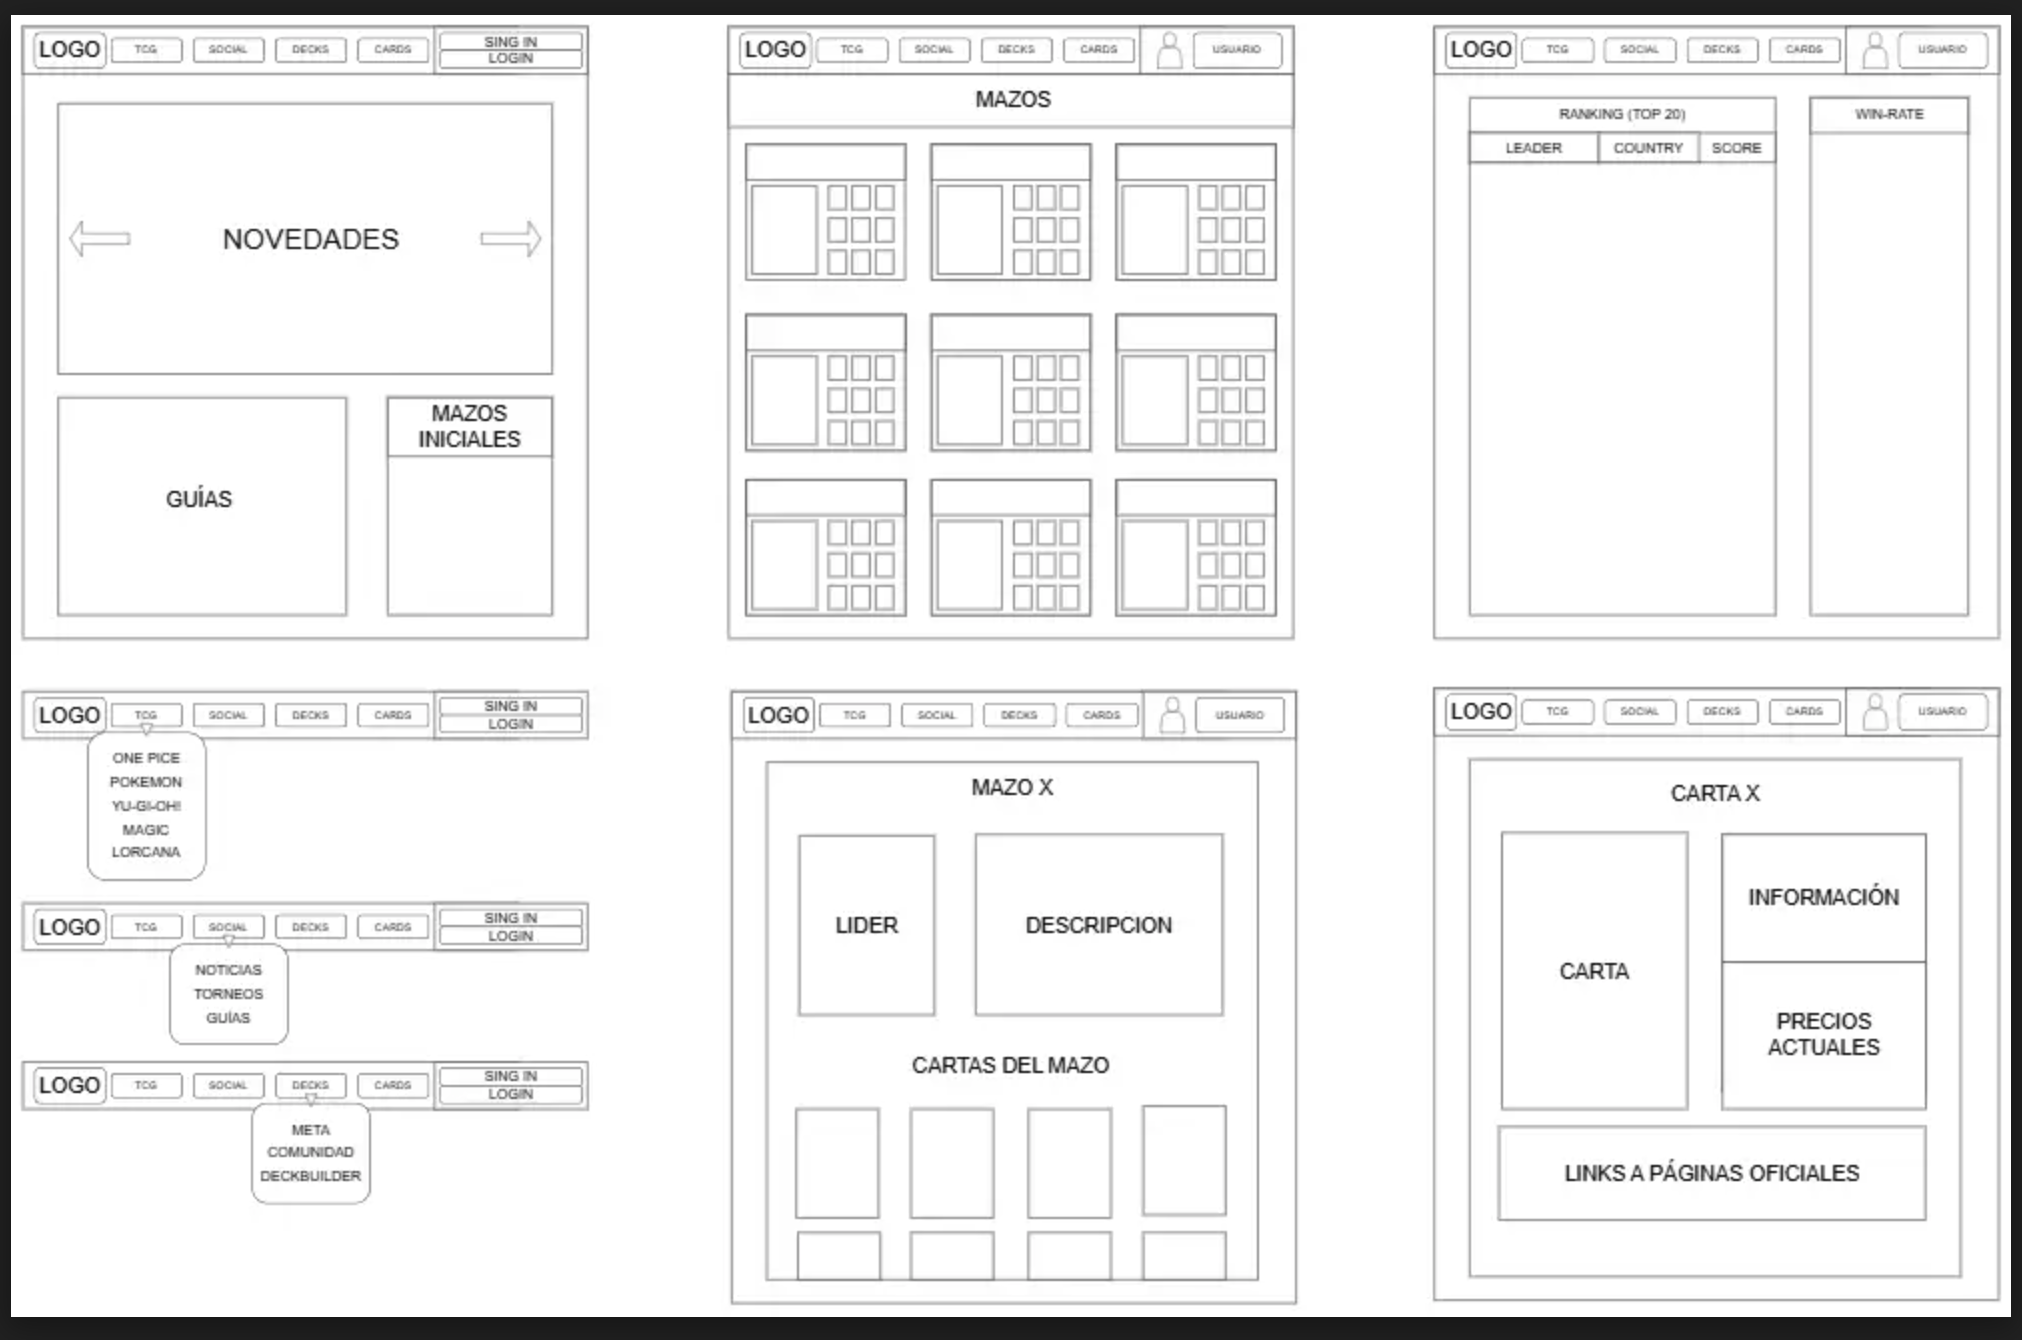
\includegraphics[width=0.85\textwidth]{Recursos/Bocetos2.png}
	%	\caption{\textbf{Boceto limpio con todas las vistas}}
	%\end{figure}
	
	\subsubsection*{Página de inicio}

	\begin{figure}[H]
		\centering
		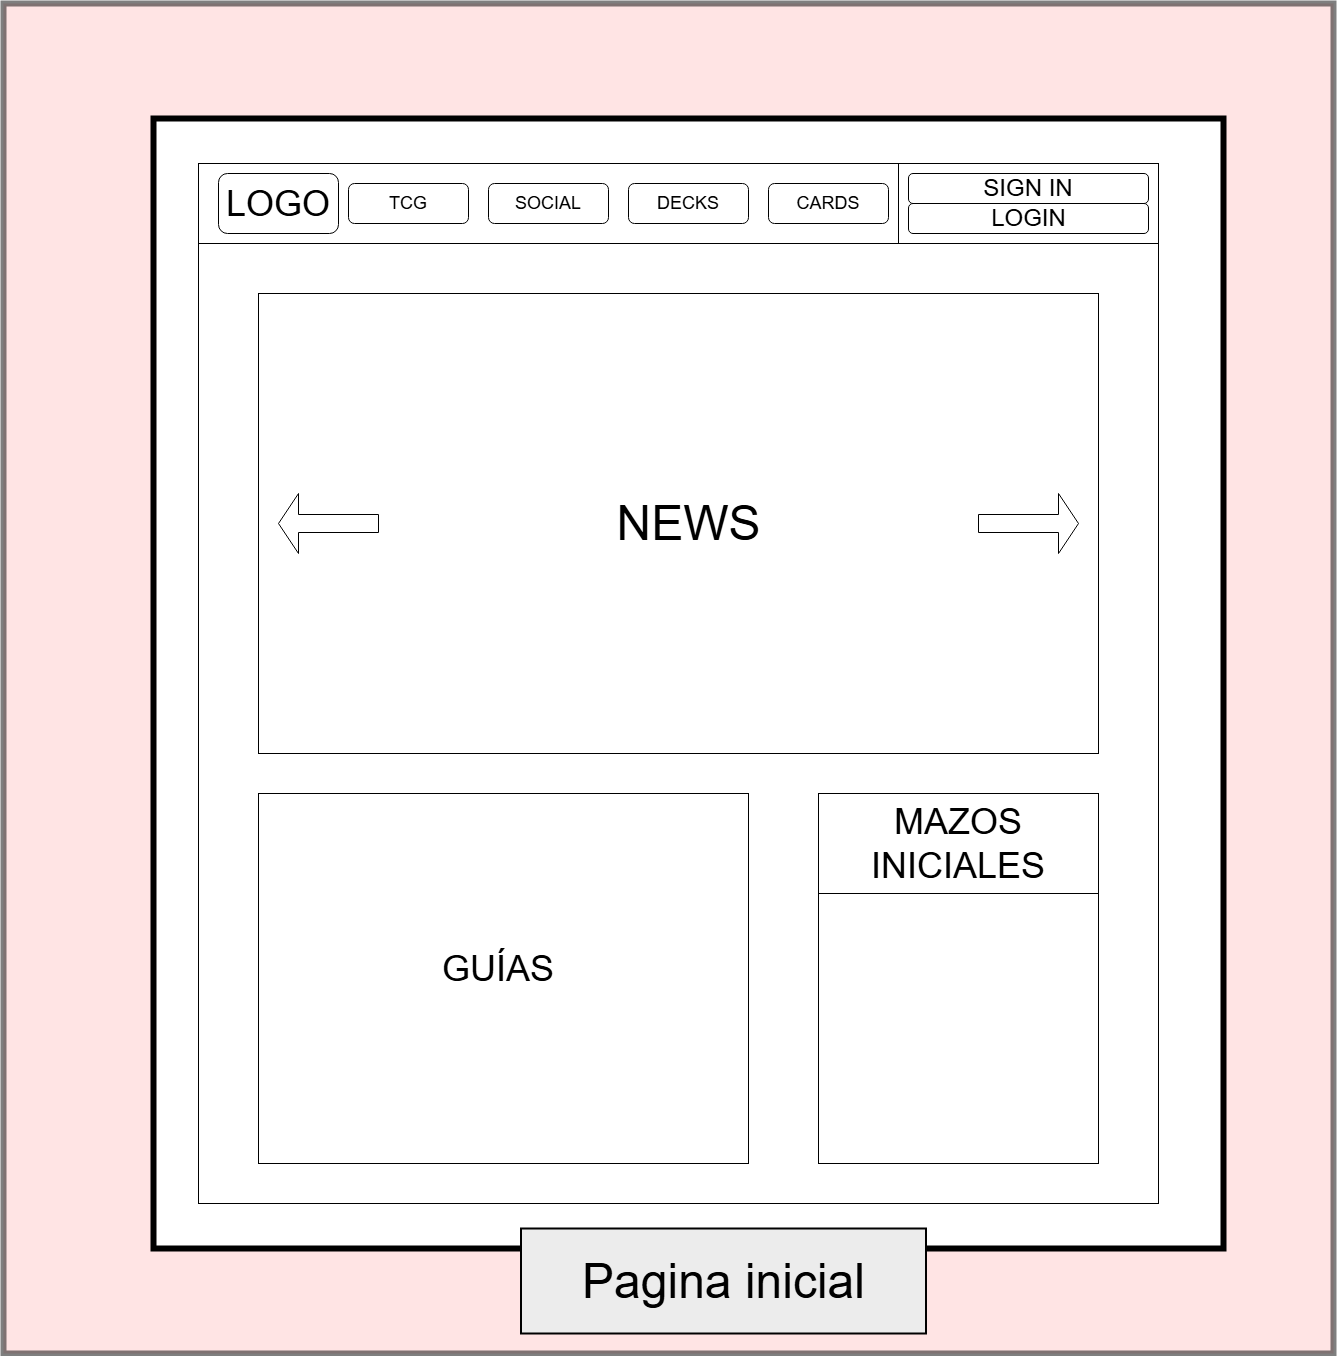
\includegraphics[width=0.85\textwidth]{Recursos/Boceto2_Inicio.png}
		\caption{\textbf{Boceto de la página de Inicio}}
	\end{figure}
	Observamos que la página inicial se compone de dos elementos clave, la barra de navegación (explicada en la siguiente captura) y los contenidos más relevantes. Hablando de los contenidos relevantes, hemos planteado que se incluya un subapartado de novedades (nuevas expansiones disponibles, información destacada sobre torneos, noticias relacionadas con el \textit{TCG}, etc.), un subapartado con las guías para principiantes y un subapartado con los mejores mazos con los que comenzar a jugar.
	
	\subsubsection*{Barra de navegación de la página}
	
	\begin{figure}[H]
		\centering
		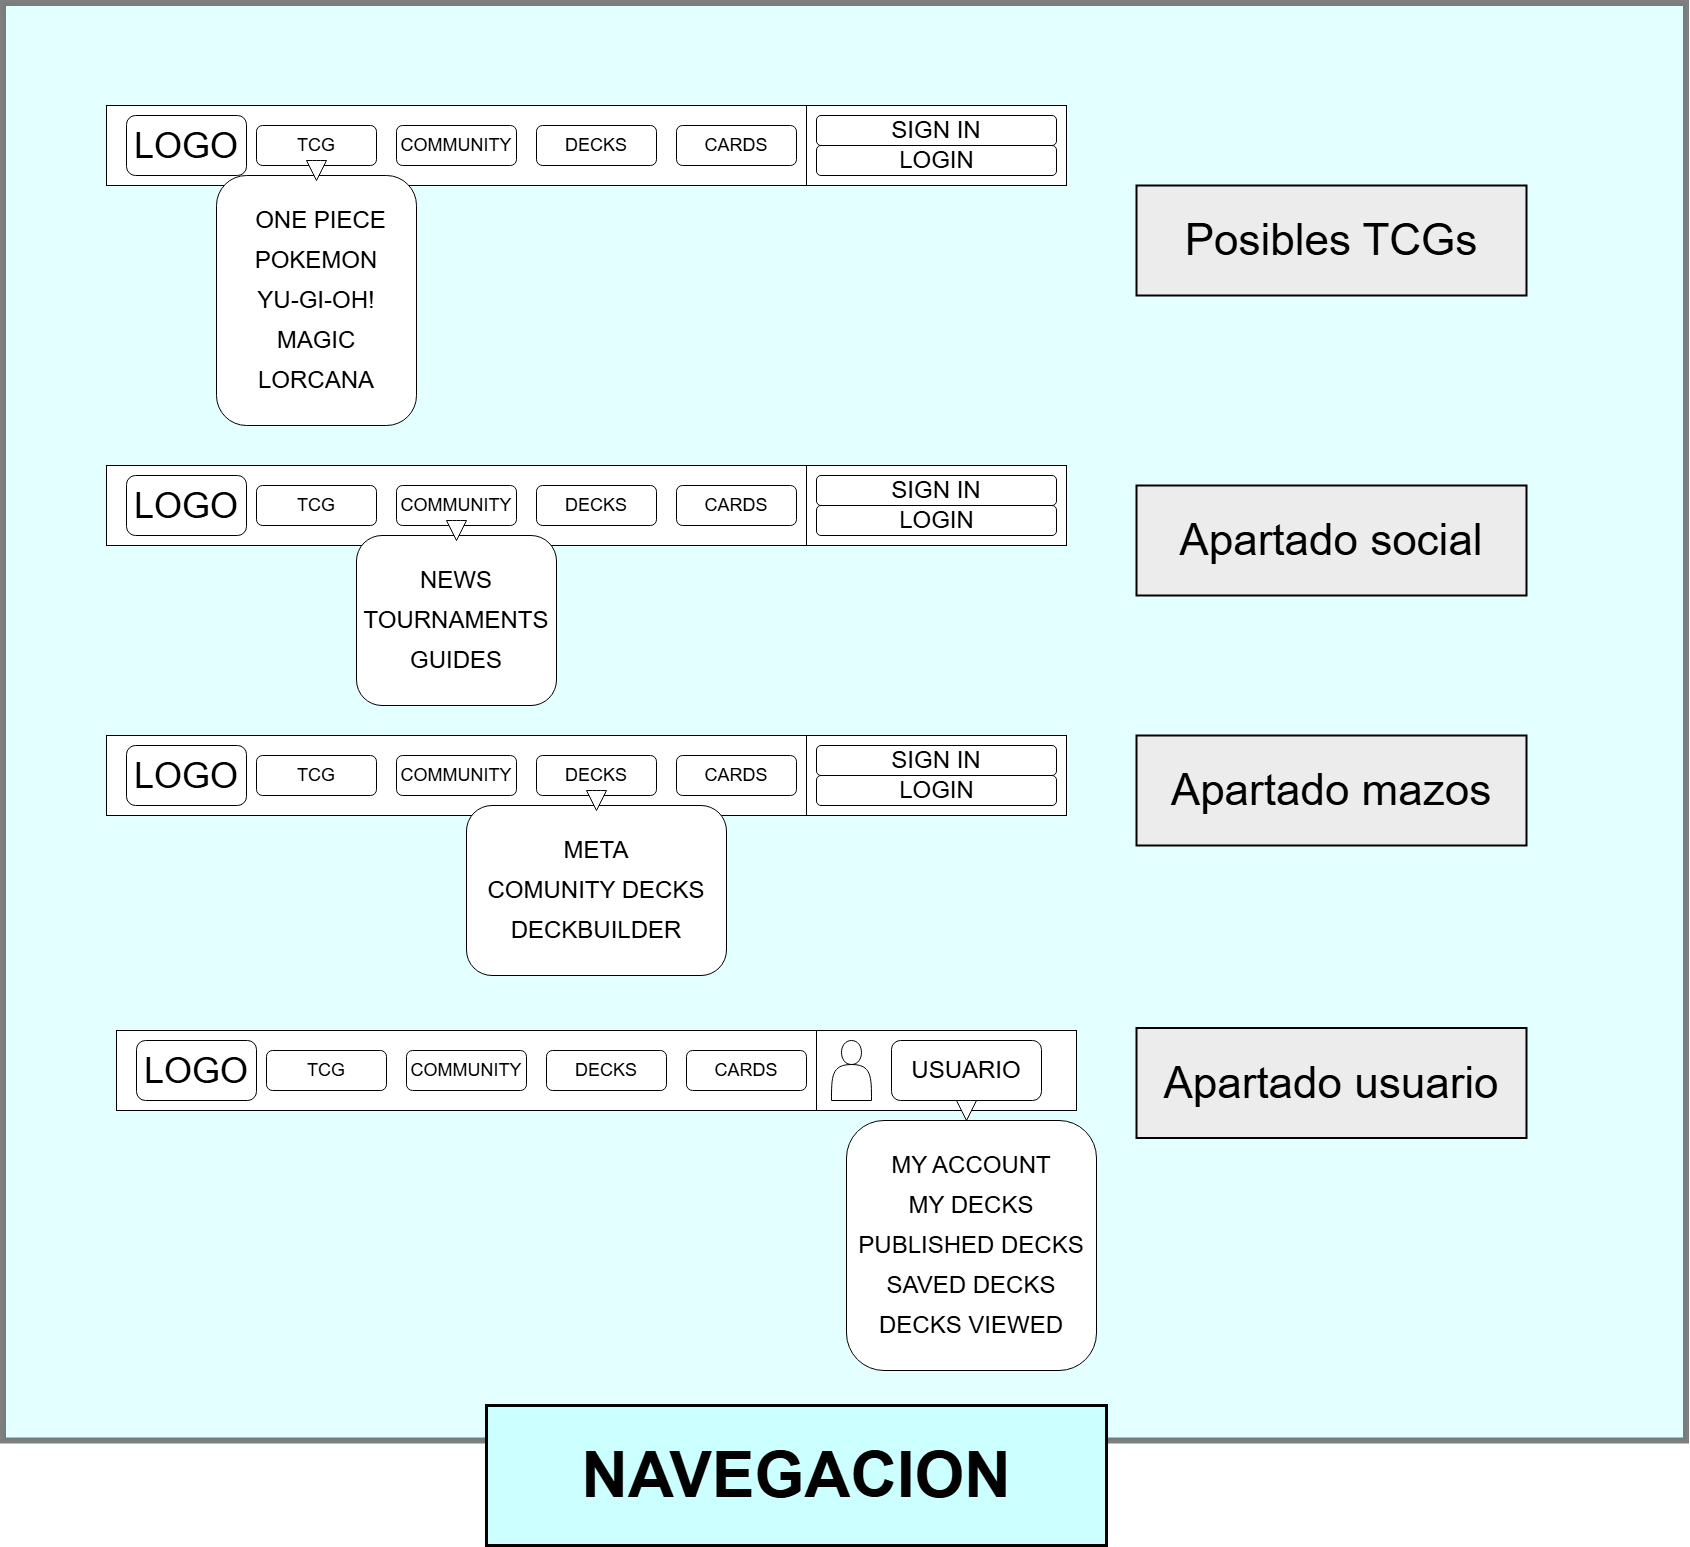
\includegraphics[width=0.85\textwidth]{Recursos/Boceto2_Navegacion.png}
		\caption{\textbf{Boceto de la barra de navegación}}
	\end{figure}
	En esta imagen observamos con más detalle la barra de navegación. Esta ayudará al usuario a navegar a través de nuestros diferentes apartados. Cada elemento abrirá diferentes submenús desplegables con las diferentes opciones disponibles. Dividiremos la barra en dos secciones: sección del juego y sección del usuario. \\
    
    Dentro de la sección del juego observamos, de izquierda a derecha, las siguientes categorías: \textit{TCG}, \textit{community} (comunidad), \textit{Decks} (mazos) y \textit{Cards} (cartas). La categoría \textit{TCG} hace referencia a los principales juegos que existen (como hemos mencionado anteriormente nos enfocaremos en el juego basado en \textit{One Piece}). En comunidad podemos acceder a las vistas relacionadas con la interacción del usuario en la comunidad: noticias, torneos y guías de usuario. La siguiente categoría, \textit{Decks}, incluye todo aquello relacionado con mazos: Mazos empleados en el \textit{META}, mazos creados por la comunidad y el creador de mazos del usuario. Por último nos encontramos con la categoría \textit{Cards}, la cual nos lleva a la lista completa de cartas existentes. \\

    Ahora hablaremos de la sección del usuario. Inicialmente vemos dos opciones, la opción de \textit{Crear cuenta}, pensada para miembros sin una cuenta existente en nuestra web; y la opción de \textit{Iniciar sesión}, enfocada a que los miembros puedan entrar a sus respectivas cuentas. Una vez iniciada la sesión cambiarán los botones a uno que despliegue un menú con las diferentes opciones: Mi cuenta, mazos creados, mazos publicados, mazos guardados e interacciones.
    
    \subsubsection*{Comunidad}
    
    \begin{figure}[H]
    	\centering
    	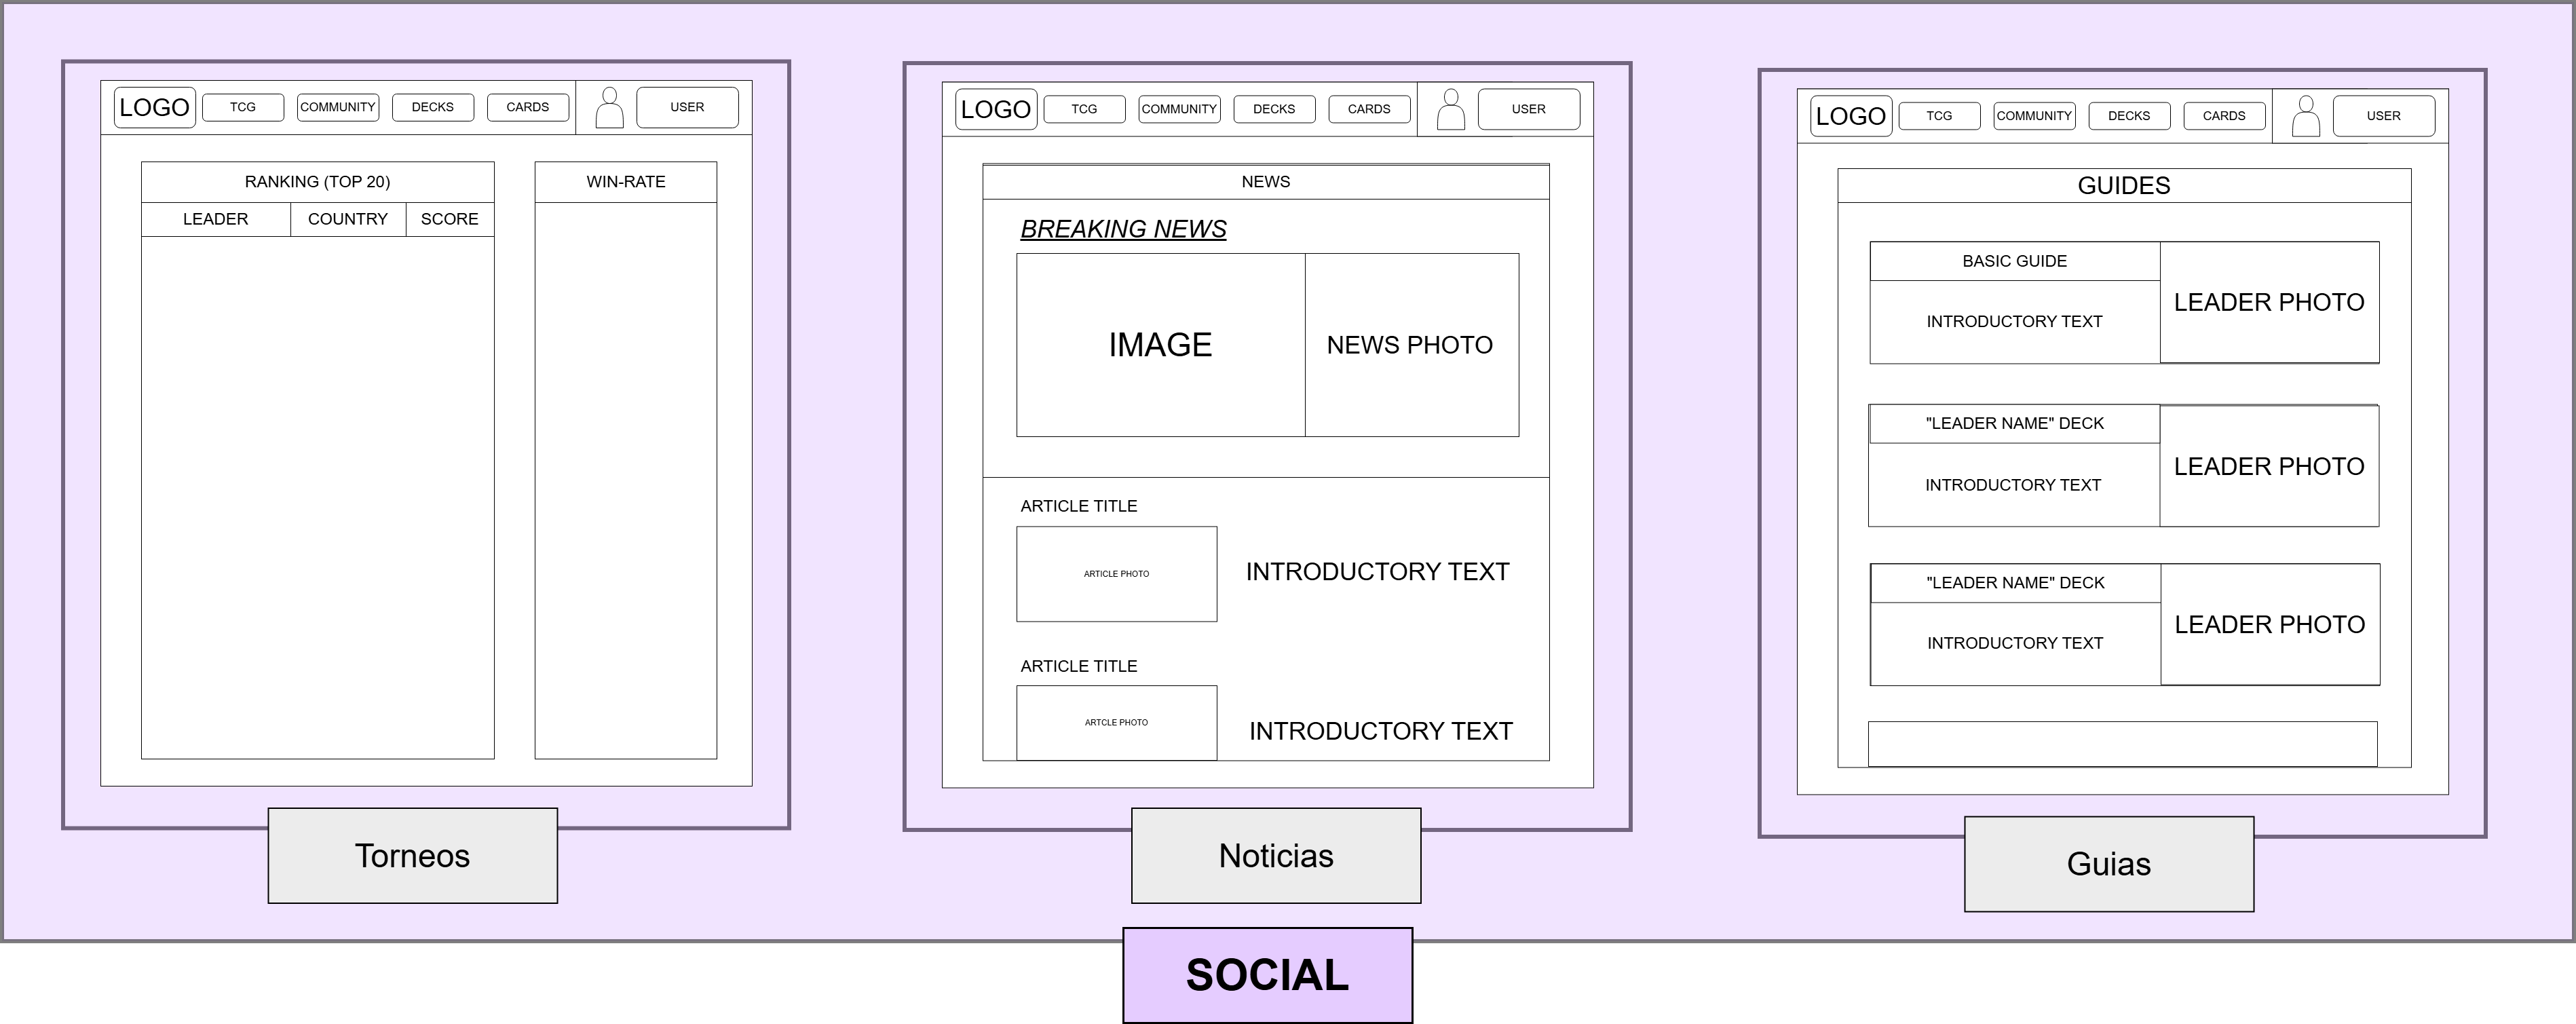
\includegraphics[width=0.85\textwidth]{Recursos/Boceto2_Social.png}
    	\caption{\textbf{Boceto de las pestañas de la comunidad}}
    \end{figure}
    
    Nos adentramos ahora en la sección de comunidad. Esta estará dividida en tres opciones diferentes: torneos, noticias y guías. \\

    En el apartado de torneos tendremos una lista con los diferentes torneos que hay (torneos pasados o futuros). Al seleccionar un torneo entramos en el visualizador del torneo, el cual se compone de dos listas, la lista de \textit{Ranking}, que muestra las posiciones de los diferentes mazos participantes en orden de su desempeño en la competición; y el apartado de \textit{Win-rate}, donde nos informará con una lista sobre el porcentaje de victorias que ha tenido cada carta líder participante. \\

    Pasamos ahora a las noticias. En esta vista nos encontramos con una lista con las noticias relacionadas con el mundo del \textit{TCG}. En la parte superior veremos las noticias con mayor relevancia, y en la parte inferior el listado con todas las noticias ordenadas por fecha más reciente. Cada noticia incluye un títular, una imagen y una pequeña sinopsis. Al hacer click en ella veremos la noticia elegida en su totalidad. \\

    Muy similar al apartado anterior, el de guias se compone de una lista con todas las guias publicadas hasta el momento. Cada noticia tiene un nombre, una breve explicación y una imagen relacionada con ella. Al seleccionar una guia se nos abrirá un visualizador completo de la guia, con sus instrucciones, imagenes explicativas e incluso vídeos informativos.
    
  	\subsubsection*{Mazos}
	
	\begin{figure}[H]
		\centering
		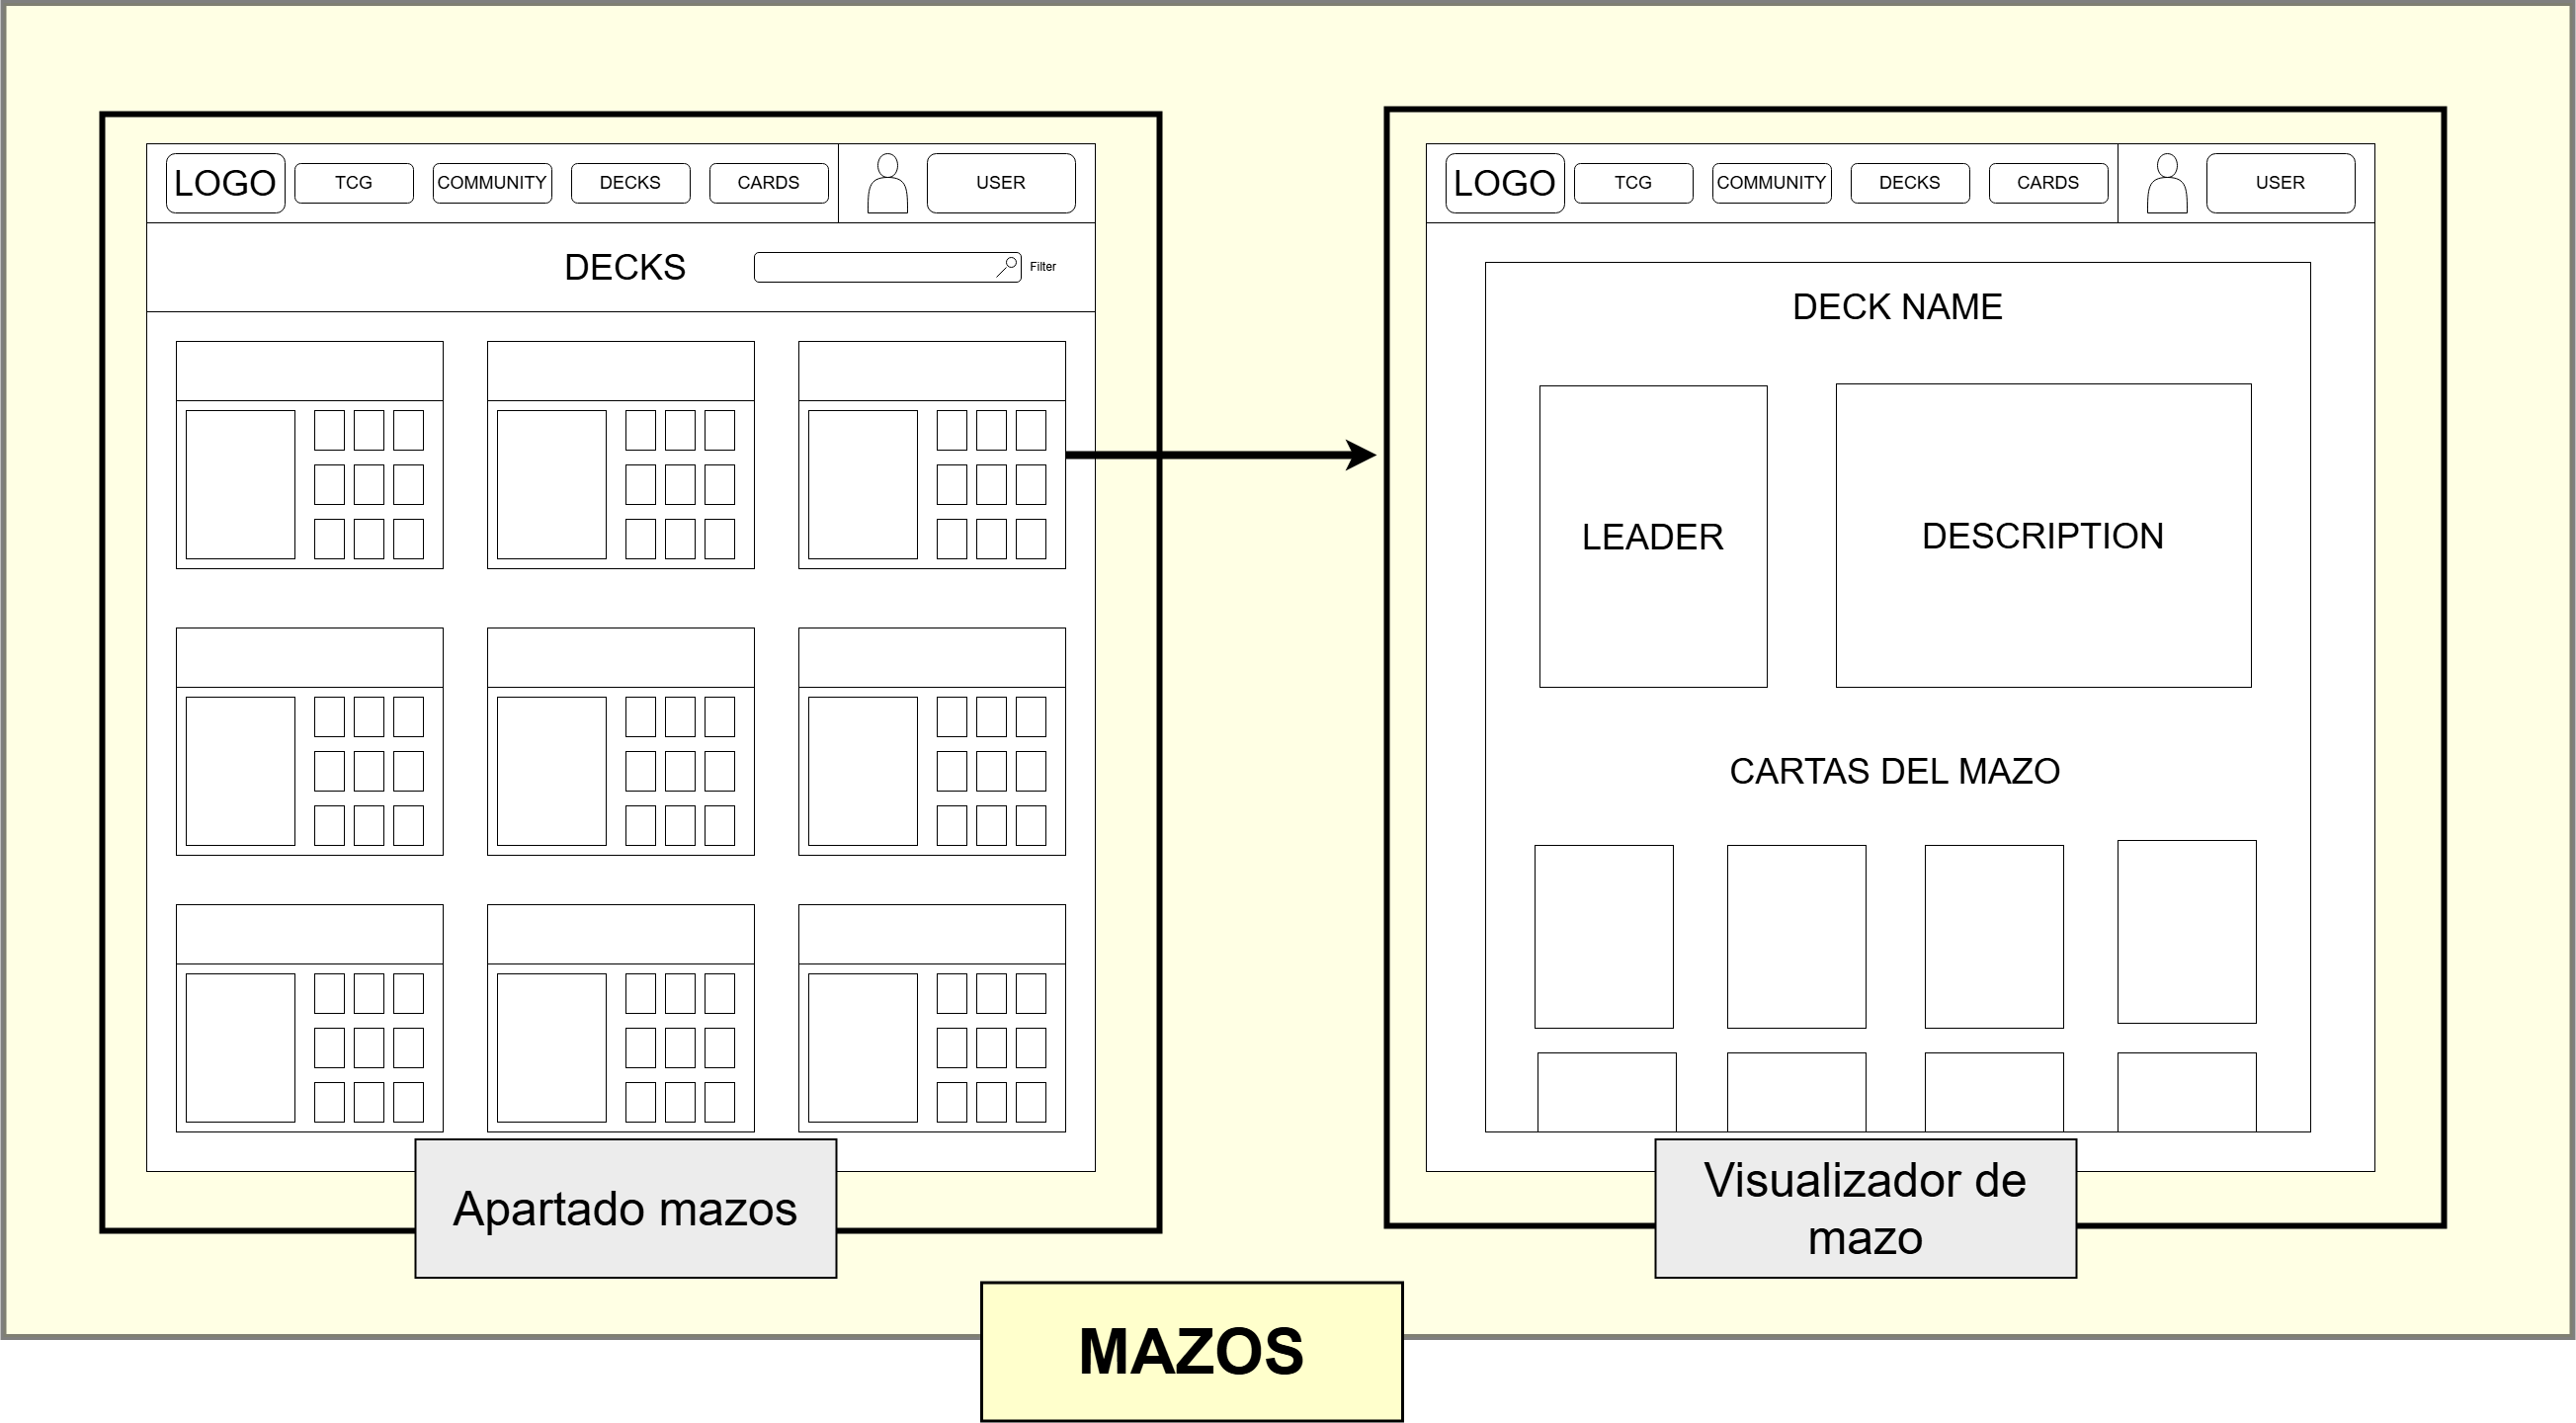
\includegraphics[width=0.85\textwidth]{Recursos/Boceto2_Mazos.png}
		\caption{\textbf{Boceto de la pestaña de mazos}}
	\end{figure}
	Esta pestaña incluye una lista con los elementos visuales de los diferentes mazos, tanto mazos \textit{META} introducidos por los administradores como los creados por la comunidad y los creados por el propio usuario, añadiendo también la opción de filtrar la búsqueda por elementos clave o buscar por nombre. Seleccionando uno se nos abre el visualizador del mazo. Aquí podemos obtener información en detalle del mismo: el nombre del mazo, la carta \textit{Líder} del mazo, una descripción de este y la lista de cartas que lo compone.
	
	\begin{figure}[H]
		\centering
		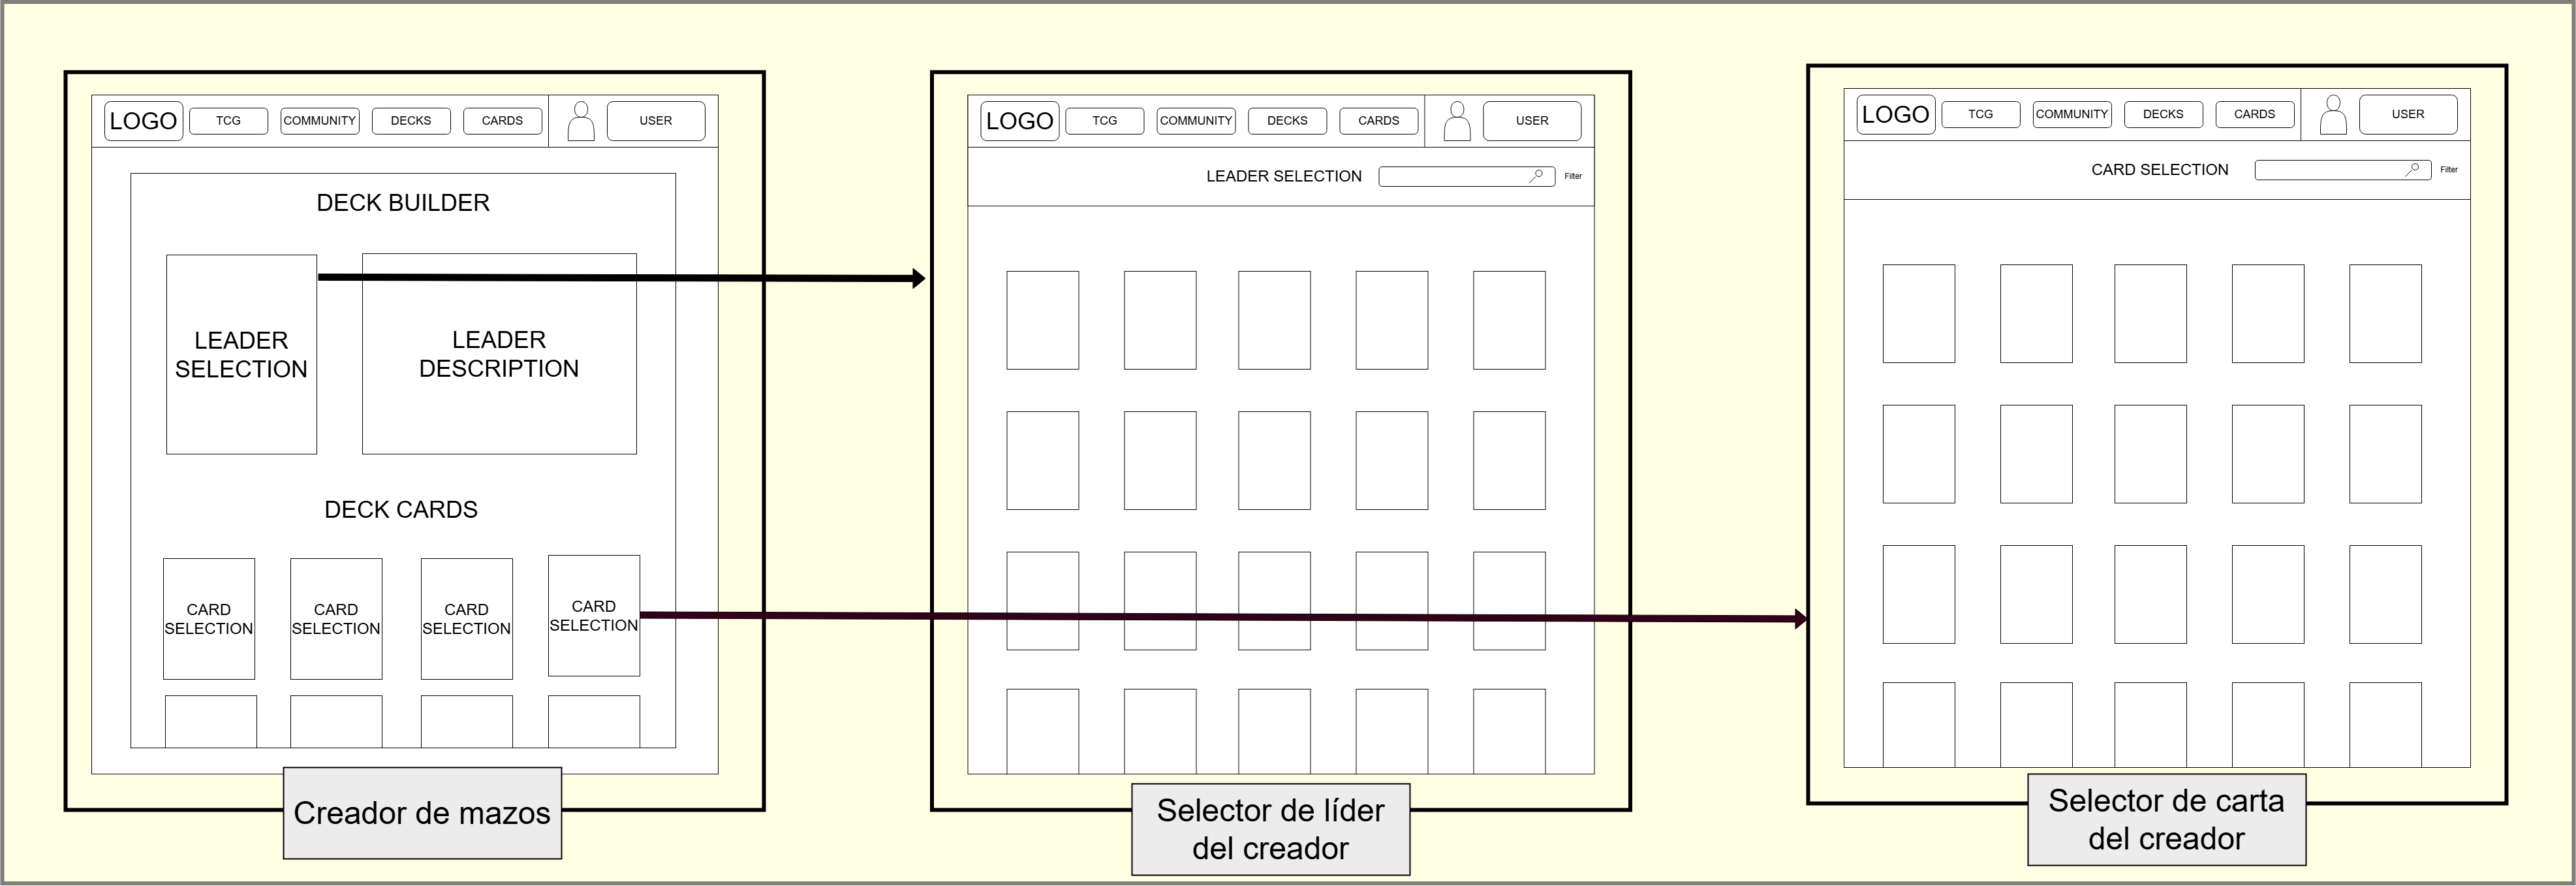
\includegraphics[width=0.85\textwidth]{Recursos/Boceto2_CreadorMazos.png}
		\caption{\textbf{Boceto de la pestaña del creador mazos}}
	\end{figure}
	Ahora observamos el apartado del creador de mazos. La vista es similar a la visualización de mazos de la comunidad, con la diferencia de que inicialmente no habrá cartas ni información de ningún tipo. \\
    
    Al seleccionar el apartado de la carta \textit{Líder} se nos abrirá un selector de cartas muy parecido a la lista entera de cartas (explicado en el siguiente apartado). Se pedirá al usuario que seleccione el color en el que esté basado el mazo que quiere crear (dentro del mundo del juego de One Piece hay cartas con diferentes colores, cada color tiene una mécanica diferente) y a raíz de eso saldrá la lista de líderes filtrada por el color seleccionado. \\
    
    De la misma forma se abrirá una lista de cartas normales al seleccionar el apartado de cartas normales, filtradas ya con el color del líder.
	
	\subsubsection*{Cartas}
	
	\begin{figure}[H]
		\centering
		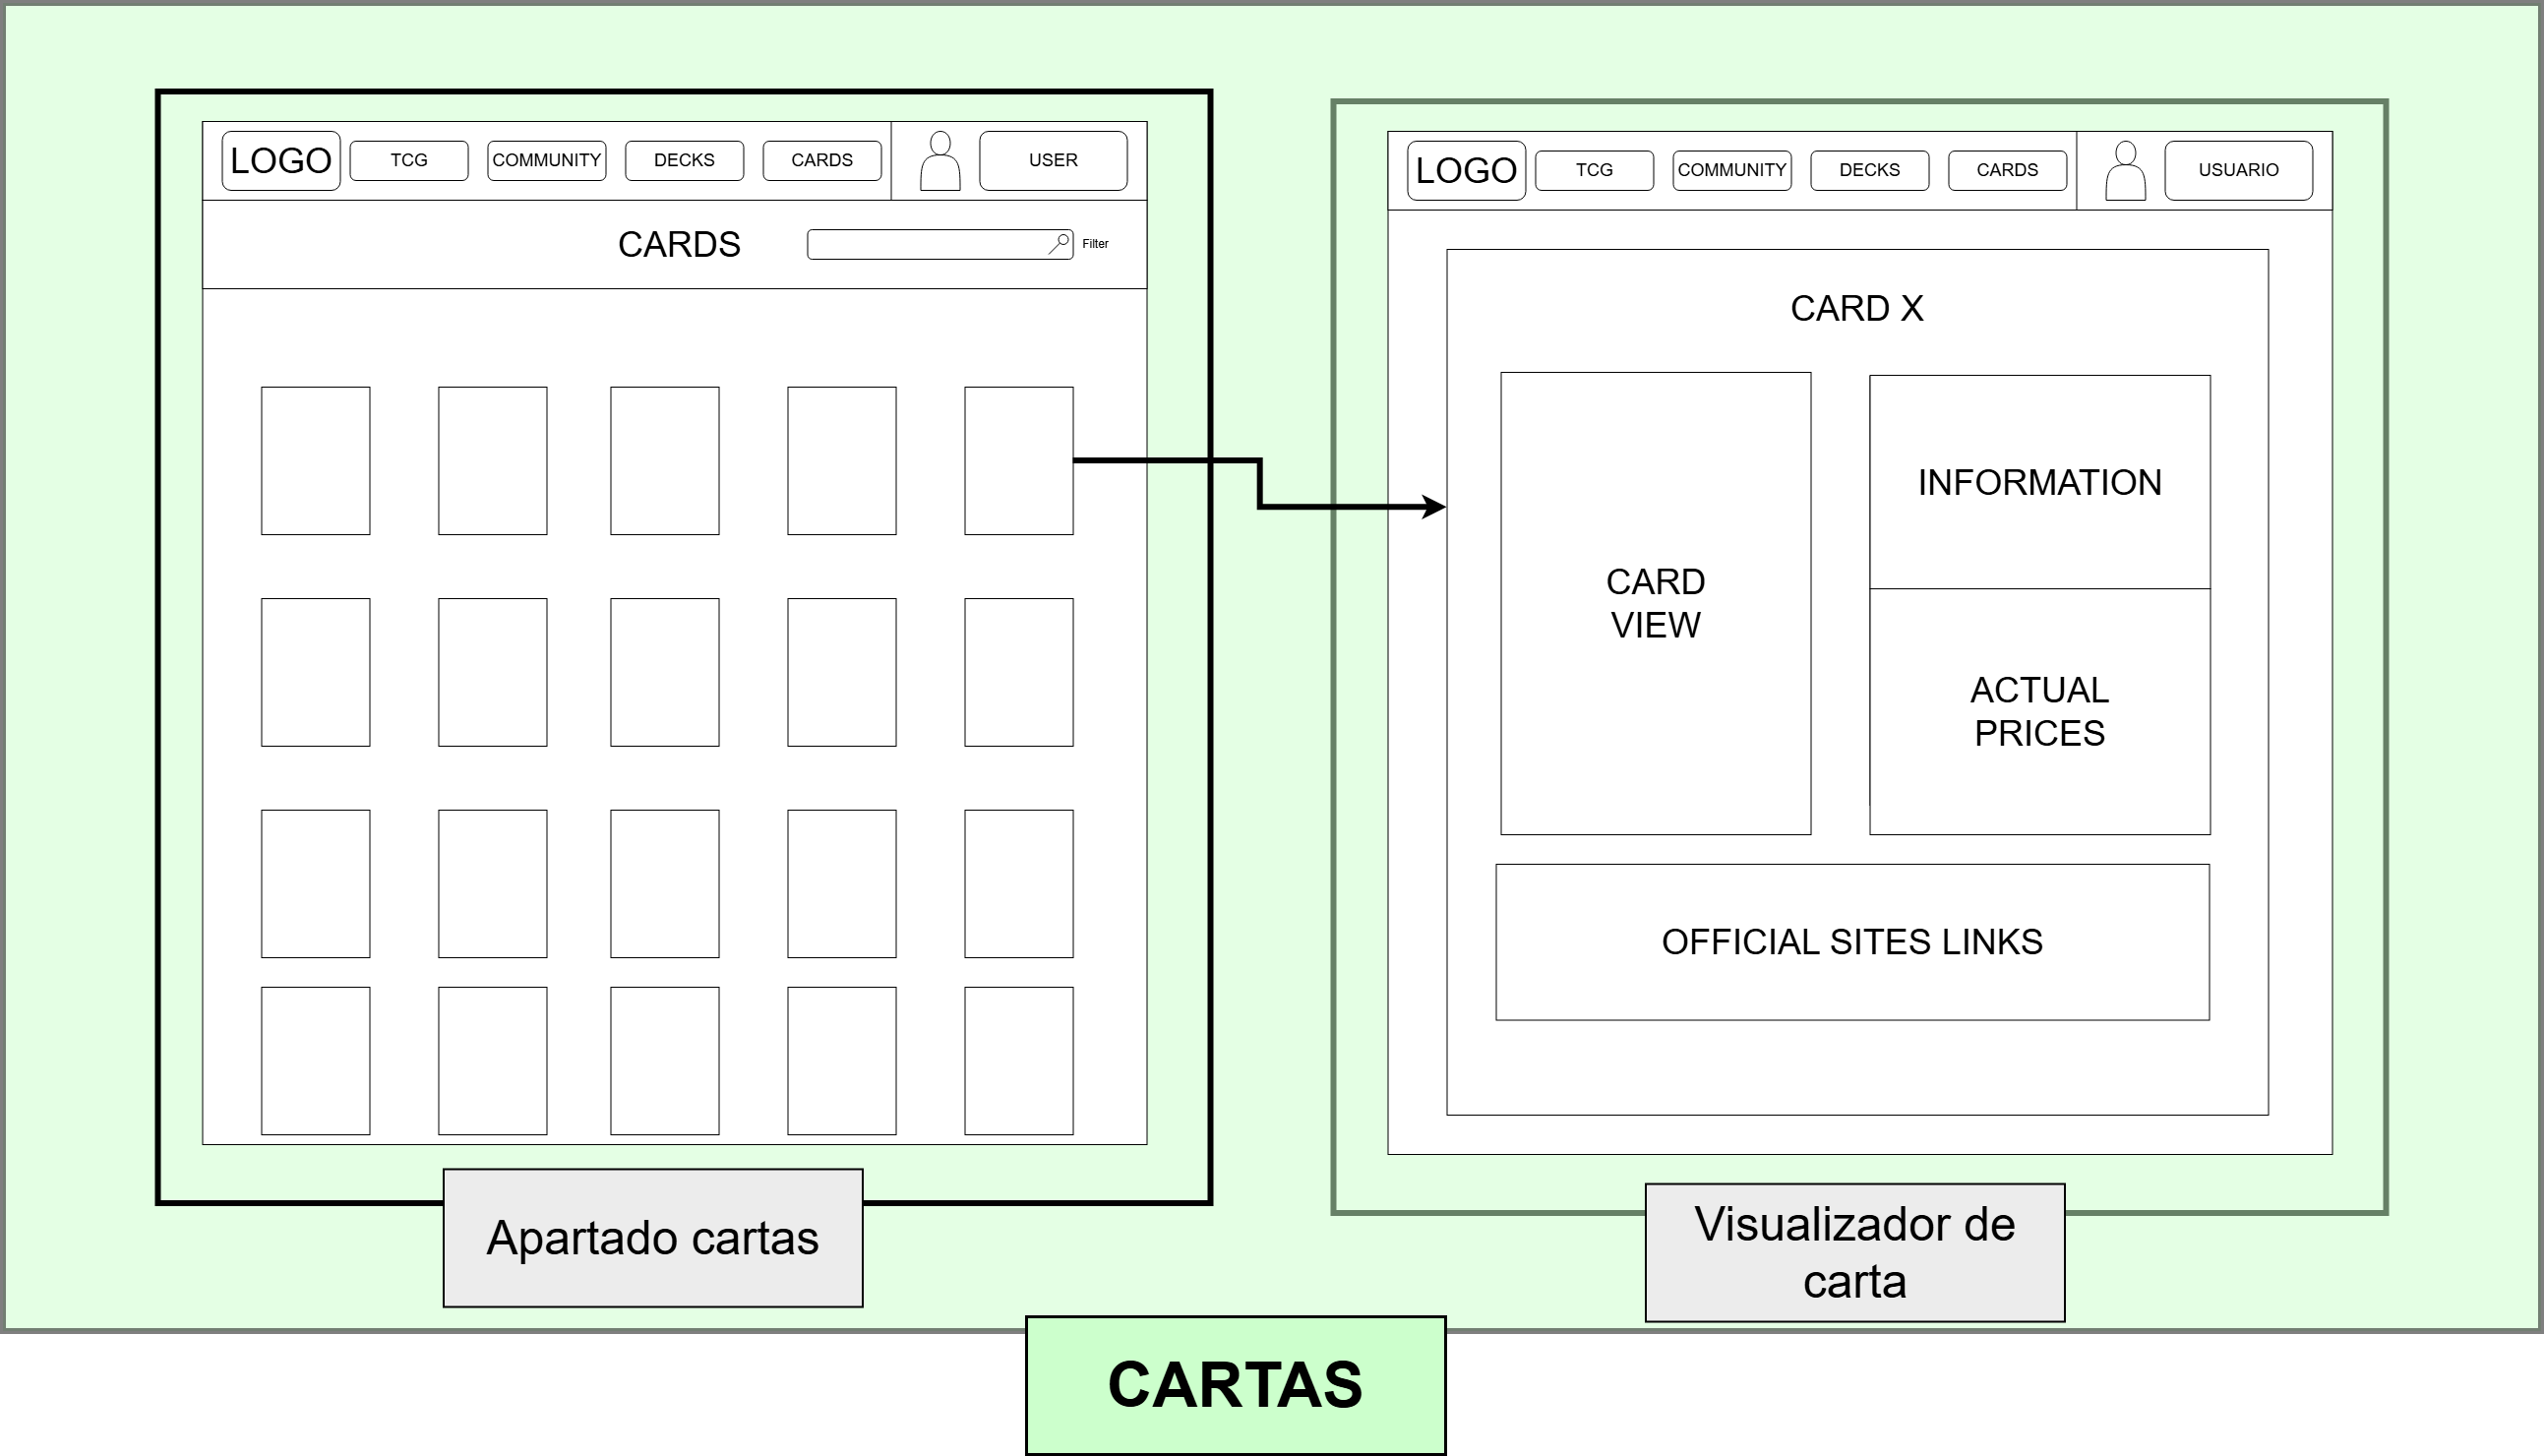
\includegraphics[width=0.85\textwidth]{Recursos/Boceto2_Cartas.png}
		\caption{\textbf{Boceto de la pestaña de cartas}}
	\end{figure}
	Similar a la pestaña de mazos, la pestaña de cartas nos incluye la lista de todas las cartas existentes. Encontramos filtros de búsqueda (color, coste, daño, mecánica, etc.) que nos ayudan a encontrar las cartas que más convengan al usuario. Si se selecciona una carta podemos visualizar información en detalle: El nombre de la carta, una imagen de ella, el texto de información que está incluido en la carta, el precio en la web de compraventa y links a la página oficial del juego relacionados con ella.
        
        
    \subsection{Alcance actual del sistema}        
        En la versión actual del proyecto hemos desarrollado \textit{Card Partner} como una aplicación web basada en JSP, Servlets, DAOs, clases de dominio y una base de datos relacional en MariaDB. La aplicación cuenta con vistas para la página principal, catálogo de cartas, visualización de carta, mazos de comunidad, mazos meta, constructor de mazos, visualización de mazo, login, registro, perfil de usuario, noticias, guías, torneos y sección TCG.\\
        
        Con esta estructura, hemos intentado mantener la idea inicial del proyecto, pero adaptándola a una implementación realista. Algunas funcionalidades se han desarrollado de forma completa, mientras que otras quedan planteadas como base para ampliaciones futuras. Aun así, el sistema actual ya permite representar los principales elementos del dominio: usuarios, cartas, mazos, artículos, comentarios, valoraciones, mazos guardados y listas de deseos.\\
        
        Esta descripción general sirve como punto de partida para los siguientes apartados del documento, donde detallamos los usuarios objetivo, los requisitos del sistema, el modelo de dominio, el mapa del sitio web, la estructura de la base de datos y las funcionalidades finalmente implementadas.

    \newpage   
		
	\section{Usuarios objetivo}       
        En esta sección definimos los perfiles de usuario a los que va destinada nuestra aplicación. Para ello, hemos distinguido dos formas de clasificar a los usuarios: según su nivel de conocimiento del TCG y según su nivel de acceso dentro del sistema.
        
    \subsection{Usuarios según su conocimiento del juego}
        En primer lugar, hemos diferenciado entre usuarios novatos y usuarios experimentados. Esta clasificación nos permite adaptar las funcionalidades de \textbf{Card Partner} a las necesidades reales de cada tipo de jugador.

        \begin{itemize}
            \item Los usuarios novatos son aquellas personas que sienten curiosidad por el juego de cartas, pero que todavía no tienen experiencia previa suficiente. Pueden llegar al TCG porque conocen la serie en la que está basado, porque algún conocido se lo ha recomendado o porque quieren iniciarse en un nuevo juego de cartas coleccionables. Para este tipo de usuario, hemos planteado secciones de guías, noticias, recomendaciones y mazos orientados a principiantes, de forma que puedan entender las reglas básicas, las mecánicas principales y las primeras decisiones necesarias para empezar a jugar.
            \item Los jugadores experimentados son usuarios que ya conocen las mecánicas del TCG y buscan herramientas más completas. Este perfil necesita consultar cartas, revisar precios, estudiar mazos meta, probar combinaciones, crear sus propios mazos y compartirlos con la comunidad. Para ellos, \textbf{Card Partner} ofrece funcionalidades como el catálogo de cartas, el constructor de mazos, los mazos de la comunidad, los mazos meta, los comentarios y las valoraciones. Con ello, hemos buscado facilitar tanto el seguimiento del entorno competitivo como la interacción entre jugadores.
        \end{itemize}

    \subsection{Usuarios según su nivel de acceso}
        Además de la clasificación anterior, hemos definido distintos tipos de usuario según las acciones que pueden realizar dentro de la aplicación. Esta segunda clasificación es necesaria porque no todos los usuarios tienen los mismos permisos ni participan de la misma forma en el sistema.
        
    \subsubsection{Visitante no registrado}
        El visitante no registrado representa al usuario que accede a la aplicación sin iniciar sesión. Este usuario puede consultar información pública de la plataforma, como el catálogo de cartas, las noticias, las guías, los torneos, los mazos meta y los mazos publicados por la comunidad. Su objetivo principal es explorar el contenido disponible antes de decidir si quiere registrarse.\\
        
        Este perfil es importante porque permite que \textbf{Card Partner} sea útil incluso para usuarios que solo desean consultar información puntual. Sin embargo, sus acciones están limitadas y no puede crear mazos, guardar contenido, comentar, valorar ni gestionar un perfil propio.
        
    \subsubsection{Jugador registrado}
        El jugador registrado es el usuario que ha creado una cuenta e iniciado sesión en la aplicación. Este perfil dispone de funcionalidades personalizadas, como la gestión del perfil, la creación de mazos, el guardado de mazos, la publicación de listas, la realización de comentarios y la valoración de mazos creados por otros usuarios.\\
        
        Este tipo de usuario constituye el núcleo de la comunidad de Card Partner. Hemos orientado gran parte de la aplicación a que pueda construir y organizar sus propios mazos, consultar los de otros jugadores y participar en la mejora del contenido compartido mediante interacciones sociales.
        
    \subsubsection{Administrador o usuario de mantenimiento}
        El administrador representa al usuario con permisos de gestión y mantenimiento dentro de la aplicación. Este perfil es necesario porque \textbf{Card Partner} no solo contiene información generada por jugadores, sino también contenido que debe ser revisado, actualizado o mantenido de forma controlada.\\
        
        Entre sus funciones se encuentran la gestión de contenidos editoriales, como noticias, guías y torneos; la revisión de información relevante para la plataforma; la actualización de mazos oficiales o meta; y el mantenimiento general de los datos del sistema. De esta forma, el administrador actúa como responsable de que la información publicada sea coherente, esté actualizada y mantenga la calidad esperada.\\
        
        Hemos decidido incluir este perfil porque una aplicación de este tipo requiere tareas de administración que no deberían depender de usuarios finales. La existencia de un rol administrativo permite separar las acciones de consulta y participación de los jugadores de las acciones de mantenimiento y gestión interna de la plataforma.
        
    \subsection{Resumen de perfiles}
        \begin{table}[H]
            \centering
            \renewcommand{\arraystretch}{1.3}
            \begin{tabular}{|p{3.5cm}|p{5cm}|p{5.5cm}|}
                \hline
                \textbf{Perfil} & \textbf{Descripción} & \textbf{Funcionalidades principales} \\
                \hline
                    Visitante no registrado & Usuario que accede sin iniciar sesión. & Consulta de cartas, mazos públicos, noticias, guías, torneos y contenido público. \\
                \hline
                    Jugador registrado & Usuario con cuenta propia dentro de la aplicación. & Gestión de perfil, creación de mazos, guardado de mazos, comentarios, valoraciones y participación en la comunidad. \\
                \hline
                    Administrador & Usuario con permisos de mantenimiento y gestión. & Gestión de noticias, guías, torneos, mazos oficiales, datos relevantes y mantenimiento general del sistema. \\
                \hline
            \end{tabular}
            \caption{Resumen de usuarios objetivo según su nivel de acceso}
        \end{table}
    	%• El grupo de usuarios a que se destine el sitio web debe ser sensato y no trivial.
    	%• Se describirá el grupo de usuarios con suficiente detalle como para poder diferenciarlo de otros.
    	%• Se describirán las necesidades y expectativas reconocidas en el grupo de usuarios objetivo.

    
		% USUARIOS (6,5/10)\\
		% Se definen dos tipos de usuario a nivel de 'usuarios finales', con los perfiles claramente definidos. No se cita ningún tipo de usuario con capacidad de administración de la aplicación a nivel de 'backend'/mantenimiento. ¿Existe? Se debe concretar, ya que se está diseñando una aplicación que, posiblemente, requerirá mantenimiento y/o actualizaciones, gestión de los contenidos,... ¿Quién lo lleva a cabo?\\
	
	\section{Especificación de requisitos}
		% La especificación de requisitos está organizada y numerada en bloques temáticos, y contiene RNF específicos y mensurables.\\
		
		% El modelo de dominio es el que está mejor resuelto: la herencia adecuada de Usuario en Jugador y Administrador, una clase asociativa Contiene con un atributo cantidad, enumeraciones particulares del dominio (tipos, colores,...), y una descripción textual que complementa de manera perfecta el diagrama.\\
		
		% El mapa del sitio, que documenta cuatro niveles de profundidad con flujos de navegación detallados, excede lo común en esta entrega. La funcionalidad casi completa la abarcan las páginas estáticas: Deck Builder con ventanas emergentes modales para elegir cartas y líder, visualizador de mazo con precio y winrate, visualizador de carta que incluye todas las características del modelo, así como tres apartados editoriales distintos.\\
		
		% Las mejoras que se deben incorporar son: agregar requisitos de información y reglas de negocio explícitas (como la composición mínima de un mazo o las limitaciones de copias por carta); crear la página del perfil del usuario, que incluya la gestión de mazos propios, ya que es el único apartado importante en el mapa que carece de una página; clarificar cómo están relacionados decks.html, community-deck.html y meta-decks.html para prevenir redundancias; y llevar a cabo el enlace con páginas específicas por juego desde la sección TCG.\\
		
		% Apartado REQUISITOS:\\
		
		% RF-1.1 menciona registro "con cuenta de Google" como alternativa, pero esto no aparece en las páginas estáticas ni en el resto del análisis. Si se mantiene como requisito, debería reflejarse en alguna página.\\
		
		% RF-5.2 ("Recomendados: Sugerencia de mazos para principiantes") no tiene una página estática propia clara; los mazos recomendados aparecen en el index pero no como sección independiente.\\

		\subsection{Requisitos funcionales}
            Los requisitos funcionales describen las acciones que los usuarios pueden realizar dentro de la aplicación. Hemos mantenido la organización por bloques temáticos para facilitar su lectura y relacionar cada requisito con una parte concreta del sistema.
            
            \noindent
            \begin{xltabular}{\textwidth}{|l|l|X|}
            	\hline
            	\rowcolor{gray!20} \textbf{ID} & \textbf{Nombre} & \textbf{Descripción} \\ \hline
            	
            	\multicolumn{3}{|c|}{\cellcolor{gray!10}\textbf{1. Gestión de usuarios y perfiles}} \\ \hline
            	RF-1.1 & Registro & El sistema permitirá crear una cuenta de usuario mediante email y contraseña, o con una cuenta de Google \\ \hline
            	RF-1.2 & Login & El sistema permitirá iniciar sesión para acceder a funcionalidades personalizadas. \\ \hline
            	RF-1.3 & Credenciales & El sistema permitirá gestionar credenciales del usuario, incluyendo el cambio de contraseña desde el perfil o desde el acceso de recuperación. \\ \hline
            	RF-1.4 & Perfil & El sistema permitirá consultar y gestionar un perfil de usuario con datos personales y mazos asociados. \\ \hline
            	
            	\multicolumn{3}{|c|}{\cellcolor{gray!10}\textbf{2. Gestión y creación de mazos}} \\ \hline
            	RF-2.1 & Deckbuilder & El sistema permitirá crear mazos mediante una herramienta interactiva de selección de carta líder y cartas del mazo. \\ \hline
            	RF-2.2 & Almacenamiento & El sistema permitirá guardar mazos asociados a un usuario registrado. \\ \hline
            	RF-2.3 & Publicación & El sistema permitirá publicar mazos para que puedan ser consultados por otros usuarios de la comunidad. \\ \hline
            	RF-2.4 & Biblioteca & El sistema permitirá mostrar los mazos creados, publicados y guardados por el usuario. \\ \hline
            	RF-2.5 & Filtro Comunidad & El sistema permitirá buscar o filtrar mazos de la comunidad según criterios como líder, nombre o características relevantes. \\ \hline
            	RF-2.6 & Estadísticas & El sistema permitirá visualizar datos de rendimiento asociados a mazos meta, como el winrate. \\ \hline
            	
            	\multicolumn{3}{|c|}{\cellcolor{gray!10}\textbf{3. Base de datos de cartas}} \\ \hline
            	RF-3.1 & Catálogo & El sistema permitirá consultar una vista general de las cartas disponibles. \\ \hline
            	RF-3.2 & Filtro avanzado & El sistema permitirá buscar cartas por atributos como nombre, color, tipo, coste o rareza, según la información disponible. \\ \hline
            	RF-3.3 & Precios & El sistema permitirá consultar el precio de mercado asociado a las cartas. \\ \hline
            	RF-3.4 & Detalle de carta & El sistema permitirá acceder a una vista detallada de una carta con sus atributos principales. \\ \hline
            	
            	\multicolumn{3}{|c|}{\cellcolor{gray!10}\textbf{4. Comunidad e interacción}} \\ \hline
            	RF-4.1 & Comentarios & El sistema permitirá a los usuarios registrados comentar mazos publicados por otros usuarios. \\ \hline
            	RF-4.2 & Valoración & El sistema permitirá valorar mazos para destacar aquellos mejor recibidos por la comunidad. \\ \hline
            	RF-4.3 & Mazos guardados & El sistema permitirá guardar mazos para consultarlos posteriormente desde el perfil del usuario. \\ \hline
            	RF-4.4 & Wishlist & El sistema permitirá asociar cartas a una lista de deseos del usuario. \\ \hline
            	
            	\multicolumn{3}{|c|}{\cellcolor{gray!10}\textbf{5. Contenido editorial y recursos}} \\ \hline
            	RF-5.1 & Noticias & El sistema permitirá consultar noticias y novedades relacionadas con el TCG. \\ \hline
            	RF-5.2 & Guías & El sistema permitirá consultar guías básicas para facilitar el aprendizaje de jugadores principiantes. \\ \hline
            	RF-5.3 & Torneos & El sistema permitirá consultar información o enlaces relacionados con eventos competitivos. \\ \hline
            	RF-5.4 & Mazos recomendados & El sistema permitirá mostrar mazos recomendados para principiantes dentro de la página principal o de secciones de apoyo al usuario novel. \\ \hline
            	
            	\multicolumn{3}{|c|}{\cellcolor{gray!10}\textbf{6. Administración y mantenimiento}} \\ \hline
            	RF-6.1 & Gestión de contenido & El sistema permitirá que usuarios administradores gestionen noticias, guías, torneos y contenido editorial. \\ \hline
            	RF-6.2 & Gestión de mazos oficiales & El sistema permitirá distinguir mazos oficiales o meta frente a mazos creados por la comunidad. \\ \hline
            	RF-6.3 & Mantenimiento de datos & El sistema permitirá mantener actualizada la información necesaria para el correcto funcionamiento de la plataforma. \\ \hline
            	
            \end{xltabular}

            \newpage
		\subsection{Requisitos no funcionales}
            Los requisitos no funcionales definen las condiciones de calidad que debe cumplir la aplicación. Hemos mantenido requisitos relacionados con rendimiento, usabilidad, seguridad, mantenibilidad y compatibilidad, adaptándolos al alcance real del proyecto.
            
            \noindent
            \begin{xltabular}{\textwidth}{|l|l|X|}
            	\hline
            	\rowcolor{gray!20} \textbf{ID} & \textbf{Nombre} & \textbf{Descripción} \\ \hline
            	
            	\multicolumn{3}{|c|}{\cellcolor{gray!10}\textbf{1. Rendimiento y eficiencia}} \\ \hline
            	RNF-1.1 & Tiempo de respuesta & El sistema deberá ofrecer tiempos de carga razonables en las vistas principales y en las búsquedas de cartas y mazos. \\ \hline
            	RNF-1.2 & Optimización & El sistema deberá evitar cargas innecesarias de recursos, especialmente en imágenes de cartas y listados extensos. \\ \hline
            	RNF-1.3 & Paginación & El sistema deberá limitar la cantidad de cartas o mazos mostrados simultáneamente para mejorar la navegación. \\ \hline
            	
            	\multicolumn{3}{|c|}{\cellcolor{gray!10}\textbf{2. Usabilidad y experiencia de usuario}} \\ \hline
            	RNF-2.1 & Diseño coherente & La interfaz deberá mantener una apariencia homogénea entre las distintas vistas. \\ \hline
            	RNF-2.2 & Navegación & El usuario deberá poder acceder a las secciones principales desde una cabecera común. \\ \hline
            	RNF-2.3 & Aprendizaje & El constructor de mazos deberá ser comprensible para usuarios que no tengan experiencia previa con herramientas similares. \\ \hline
            	
            	\multicolumn{3}{|c|}{\cellcolor{gray!10}\textbf{3. Seguridad y privacidad}} \\ \hline
            	RNF-3.1 & Protección de datos & El sistema deberá proteger la información personal de los usuarios y evitar exponer datos sensibles innecesariamente. \\ \hline
            	RNF-3.2 & Control de acceso & Las funcionalidades personalizadas deberán requerir que el usuario haya iniciado sesión. \\ \hline
            	RNF-3.3 & Validación & El sistema deberá validar los datos recibidos desde formularios para reducir errores e inserciones no válidas. \\ \hline
            	
            	\multicolumn{3}{|c|}{\cellcolor{gray!10}\textbf{4. Disponibilidad y mantenibilidad}} \\ \hline
            	RNF-4.1 & Base de datos local reproducible & El sistema deberá poder desplegar su base de datos en local mediante scripts de creación e inserción. \\ \hline
            	RNF-4.2 & Modularidad & La aplicación deberá mantener una separación clara entre vistas JSP, Servlets, DAOs, modelos y base de datos. \\ \hline
            	RNF-4.3 & Actualización & La estructura deberá facilitar la incorporación de nuevas cartas, mazos o artículos sin rediseñar por completo el sistema. \\ \hline
            	
            	\multicolumn{3}{|c|}{\cellcolor{gray!10}\textbf{5. Compatibilidad y portabilidad}} \\ \hline
            	RNF-5.1 & Navegadores & La aplicación deberá ser accesible desde navegadores actuales como Chrome, Firefox, Edge o Safari. \\ \hline
            	RNF-5.2 & Entorno de ejecución & La aplicación deberá poder ejecutarse en un entorno local con Apache NetBeans, Tomcat y MariaDB. \\ \hline
            	RNF-5.3 & Automatización & El proyecto deberá incluir scripts que faciliten la creación de la base de datos en distintos sistemas operativos. \\ \hline
            	
            \end{xltabular}

            \subsection{Requisitos de información}
                Los requisitos de información describen los datos que el sistema debe almacenar y gestionar para que las funcionalidades anteriores puedan llevarse a cabo. Hemos definido estos requisitos a partir del modelo de dominio y de la estructura de la base de datos implementada.
                
                \noindent
                \begin{xltabular}{\textwidth}{|l|l|X|}
                	\hline
                	\rowcolor{gray!20} \textbf{ID} & \textbf{Entidad} & \textbf{Información gestionada} \\ \hline
                	
                	RI-1 & Usuario & El sistema almacenará identificador, apodo, email, contraseña, avatar, rol y fecha de registro de cada usuario. \\ \hline
                	RI-2 & Carta & El sistema almacenará identificador oficial, nombre, imagen, tipo, arquetipo, color, coste, poder, atributo y precio de cada carta. \\ \hline
                	RI-3 & Mazo & El sistema almacenará identificador, nombre, descripción, fecha de creación, visibilidad, oficialidad, winrate, usuario creador y carta líder. \\ \hline
                	RI-4 & Contenido de mazo & El sistema almacenará la relación entre mazos y cartas, incluyendo la cantidad de copias de cada carta dentro del mazo. \\ \hline
                	RI-5 & Comentario & El sistema almacenará contenido, fecha de creación, fecha de edición, usuario autor y mazo al que pertenece el comentario. \\ \hline
                	RI-6 & Valoración & El sistema almacenará la puntuación que un usuario asigna a un mazo y la fecha de dicha valoración. \\ \hline
                	RI-7 & Artículo & El sistema almacenará título, descripción, categoría, fecha de creación, fecha de edición, enlace externo, portada y administrador autor. \\ \hline
                	RI-8 & Mazo guardado & El sistema almacenará la relación entre usuarios y mazos guardados. \\ \hline
                	RI-9 & Wishlist & El sistema almacenará la relación entre usuarios y cartas añadidas a su lista de deseos. \\ \hline
                	
                \end{xltabular}

        \subsection{Reglas de negocio}
            Las reglas de negocio recogen las restricciones propias del dominio que deben cumplirse para que la información gestionada sea coherente. Hemos incluido estas reglas para concretar mejor el comportamiento esperado del sistema y evitar ambigüedades en la gestión de usuarios, cartas y mazos.
            
            \noindent
            \begin{xltabular}{\textwidth}{|l|X|}
                \hline
                \rowcolor{gray!20} \textbf{ID} & \textbf{Regla de negocio} \\ \hline
                
                RN-1 & Todo usuario registrado debe tener un email único, un apodo identificable y un rol asociado dentro del sistema. \\ \hline
                RN-2 & Solo los usuarios registrados pueden crear mazos, guardar mazos, comentar, valorar o añadir cartas a la wishlist. \\ \hline
                RN-3 & Todo mazo debe tener una carta líder asociada. \\ \hline
                RN-4 & Todo mazo debe estar asociado a un usuario creador. \\ \hline
                RN-5 & Un mazo puede ser público o privado, según decida su creador. \\ \hline
                RN-6 & Un mazo puede ser de comunidad u oficial/meta. Esta distinción se representa mediante el atributo de oficialidad del mazo. \\ \hline
                RN-7 & La relación entre mazo y carta debe almacenar la cantidad de copias de cada carta incluida. \\ \hline
                RN-8 & Las cartas deben identificarse mediante su código oficial para facilitar su relación con fuentes externas y evitar duplicados. \\ \hline
                RN-9 & Los comentarios deben almacenar tanto la fecha de creación como la fecha de edición para diferenciar cuándo se publicaron y cuándo fueron modificados. \\ \hline
                RN-10 & Cada artículo debe pertenecer a una categoría concreta: noticia, guía o torneo. \\ \hline
                RN-11 & Los mazos guardados por un usuario podrán corresponder a mazos públicos de la comunidad o a mazos oficiales/meta visibles en la aplicación. \\ \hline
                RN-12 & Las funcionalidades de administración y mantenimiento quedan reservadas a usuarios con rol administrativo. \\ \hline
                
            \end{xltabular}

    \newpage

	\section{Modelo del dominio}
        \subsection*{Descripción de las entidades}
        
        \subsection{Usuarios y roles}
        \begin{itemize}
            \item \textbf{Usuario:} La clase Usuario representa la información de acceso y autenticación del usuario registrado en la web.\\
            \textbf{Atributos:}
            \begin{itemize}
                \item id\_usuario : Identificador único del sistema
                \item apodo\_usuario : Nombre público elegido por el usuario
                \item email : Cuenta de correo electrónico asociada a la cuenta
                \item contrasena : Credencial del usuario (cifrada)
                \item fecha\_registro : Fecha de creación de la cuenta
                \item avatar : Ruta a la imagen pública del perfil del usuario
                \item rol : Tipo de rol que determina los privilegios dentro de la web
            \end{itemize}
            
            \textbf{Relaciones:}
            \begin{itemize}
                \item Crea(n:m) con MazoComunidad : El Usuario puede crear mazos y publicarlos en la web
                \item Guarda(n:m) con Mazo : El Usuario puede guardar únicamente mazos visibles, es decir, mazos públicos de la comunidad o mazos oficiales/meta. No puede guardar mazos privados de otros usuarios.
                \item Escribe (1:n) con Comentario : El Usuario puede publicar comentarios en los mazos
                \item Valora (n:m) con Mazo : El Usuario puede dar una valoración en los mazos
                \item Publica(n:m) con MazoOficial : Solo usuarios con rol ADMIN pueden publicar mazos oficiales/meta
                \item Publica(n:m) con Articulo : Solo usuarios con rol ADMIN pueden publicar artículos (Noticias, Guías o Torneos)
            \end{itemize}
        \end{itemize}
        
        \subsection{Cartas}
        \begin{itemize}
            \item \textbf{Carta:} La clase Carta representa la entidad central del TCG y su información estática.\\
            \textbf{Atributos:}
            \begin{itemize}
                \item id\_carta : Código oficial de la carta
                \item nombre\_carta : Nombre de la carta
                \item imagen\_enlace : Ruta a la ilustración de la carta
                \item tipo : Clasificación de la carta dentro del TCG de One Piece
                \item arquetipo : Familia a la que pertenece la carta (pueden ser varias)
                \item color : Clasificación de la carta dentro del TCG de One Piece
                \item coste : Puntos necesarios para jugar la carta
                \item poder : Puntos de ataque de la carta
                \item atributo : Estilo de combate de la carta
                \item precio\_mercado : Valor real de la carta
            \end{itemize}
            \textbf{Relaciones:}
            \begin{itemize}
                \item Lidera(1:1) con Mazo : Identifica a la única carta líder obligatoria de un mazo
                \item ContieneCarta(n:m) con Mazo : Identifica las cartas que componen un mazo, con cantidad
            \end{itemize}
        \end{itemize}
        
        \subsection{Mazos}
        \begin{itemize}
            \item \textbf{Mazo:} La clase Mazo representa la estructura común de cualquier mazo publicado en la web.\\
            \textbf{Atributos:}
            \begin{itemize}
                \item id\_mazo : Identificador único del sistema
                \item nombre\_mazo : Título asignado por el creador
                \item descripcion : Texto explicativo del creador
                \item fecha\_creacion : Fecha de creación del mazo
                \item precio\_total : Precio total de todas las cartas que lo componen
            \end{itemize}
            \textbf{Relaciones:}
            \begin{itemize}
                \item Usuario: Guarda y Valora
                \item Carta: Lidera y ContieneCarta
                \item Comentario: Pertenece
            \end{itemize}
            
            \item \textbf{MazoComunidad:} La clase MazoComunidad representa aquellos mazos que han sido creados por un Usuario con rol JUGADOR.\\
            \textbf{Atributos:}
            \begin{itemize}
                \item es\_publico : Identifica si el usuario creador ha hecho el mazo público o es privado
            \end{itemize}
            \textbf{Relaciones:}
            \begin{itemize}
                \item Usuario: Crea
            \end{itemize}
            
            \item \textbf{MazoOficial:} La clase MazoOficial representa aquellos mazos creados por un Usuario con rol ADMIN y contiene datos verificados del entorno competitivo.\\
            \textbf{Atributos:}
            \begin{itemize}
                \item winrate : Porcentaje de victorias del mazo en competiciones oficiales
            \end{itemize}
            \textbf{Relaciones:}
            \begin{itemize}
                \item Usuario: Publica
            \end{itemize}
            
            \item \textbf{ContieneCarta:} Clase asociativa que representa la cantidad de copias de cada carta en un mazo.\\
            \textbf{Atributos:}
            \begin{itemize}
                \item cantidad : Número de copias de la carta dentro del mazo
            \end{itemize}
        \end{itemize}
        
        \subsection{Interacción del usuario}
        \begin{itemize}
            \item \textbf{Comentario:} Representa la publicación que un Usuario deja en un Mazo.\\
            \textbf{Atributos:}
            \begin{itemize}
                \item id\_comentario : Identificador único
                \item contenido : Texto redactado por el usuario
                \item fecha\_creacion : Fecha de creación del comentario
                \item fecha\_edicion : Fecha de última edición
            \end{itemize}
            \textbf{Relaciones:}
            \begin{itemize}
                \item Mazo: Pertenece
            \end{itemize}
            
            \item \textbf{Valoracion:} Clase asociativa entre Usuario y Mazo.\\
            \textbf{Atributos:}
            \begin{itemize}
                \item fecha\_valoracion : Fecha de la valoración
                \item puntuacion : Valor numérico asignado
            \end{itemize}
        \end{itemize}
        
        \subsection{Contenido social}
        \begin{itemize}
            \item \textbf{Articulo:} Contenidos publicados por Usuarios con rol ADMIN.\\
            \textbf{Atributos:}
            \begin{itemize}
                \item id\_articulo : Identificador único
                \item titulo : Titular del artículo
                \item descripcion : Resumen del contenido
                \item categoria : Tipo de artículo (Noticia, Guia, Torneo)
                \item fecha\_creacion : Fecha de creación
                \item fecha\_edicion : Fecha de última edición
                \item enlace\_externo : URL de referencia
                \item portada : Ruta de imagen miniatura
            \end{itemize}
            \textbf{Relaciones:}
            \begin{itemize}
                \item Usuario(ADMIN): Publica
            \end{itemize}
        \end{itemize}

        \subsection*{Diagrama del Modelo del dominio}	
        	\begin{figure}[H]
        		\centering
        		\includegraphics[width=0.9\textwidth]{SSW/Recursos/ModeloDominio_Grupo33.png}
        		\caption{Diagrama UML del Modelo de Dominio de Card Partner}
        		\label{fig:modelo_dominio}
        	\end{figure}
        		
		% Apartado MODELO DOMINIO:\\
		
		% No se modela la fecha de registro del usuario ni la fecha del comentario (solo fecha\_edicion). Para una web social es relevante distinguir cuándo se creó algo de cuándo se editó por última vez.\\
		
		% La relación Guarda entre Jugador y Mazo debería especificar si el jugador puede guardar únicamente mazos públicos de la comunidad o también mazos META oficiales. La multiplicidad está definida pero la restricción semántica no\\
		
		% No se modela la relación entre Articulo y las categorías (Noticia, Guía, Torneo) como una enumeración dentro de Articulo con categoria : CategoriaArticulo, cuando en el diagrama sí aparece correctamente. La descripción no lo menciona explícitamente.\\

	\section{Diseño del mapa del sitio web}
	\subsection*{Descripción del mapa del sitio web}
	El mapa del sitio web define la jerarquía de navegación y la reutilización de vistas y centralización de las herramientas. La estructura está diseñada para facilitar el acceso rápido a las diferentes herramientas de \textbf{Card Partner} a través de su menú de navegación en la barra superior de la página, disponible en cualquier momento.\\
	
	El mapa está estructurado en 4 niveles de profundidad para facilitar una entrada sencilla y estructurada a las herramientas:.\\
	\begin{itemize}
		\item \textbf{Nivel 0: Punto de entrada}\\
			El nivel 0 es la base de la estructura de la web, la \textbf{Página Principal} y es el punto de entrada de los usuarios. Desde ahí se muestra accesos rápidos a diferentes subsecciones de la web que pueden ser interesantes para usuarios nuevos o novedades para los usuarios experimentados.\\
		\item \textbf{Nivel 1: Navegación global}\\
			El nivel 1 es la base de la navegación dentro de la web. El \textbf{Menú de navegación} es la barra de navegación accesible en todo momento que divide la web en 4 grandes secciones, correspondientes al nivel 2 que son las herramientas para el usuario\\
		\item \textbf{Nivel 2: Herramientas y listados}\\
			El nivel 2 son las diferentes herramientas y visualización de contenido que ofrece la web a los usuarios, que se han dividido en 4 secciones:
			\begin{itemize}
				\item \textbf{SOCIAL:} Este apartado mostrará 3 subsecciones que llevarán al \textbf{Listado de Artículos} que mostrará contenidos de  categorías de artículos diferentes (Noticias, Guías o Torneos) según desde dónde se acceda, y haciendo click en el artículo se redirigirá al usuario al sitio externo referido del artículo.
				\item \textbf{CARTAS:} Este apartado llevará directamente al \textbf{Listado de cartas}, página donde se mostrarán las cartas del TCG y se podrá acceder a cada una de ellas, dirigiendo al \textbf{Visualizador de carta} que mostrará más información en detalle sobre la carta seleccionada.
				\item \textbf{MAZOS:} Este apartado agrupa las herramientas referidas a los mazos; el \textbf{Creador de mazos} que es la herramienta que permitirá al usuario crear su propio mazo eligiendo las cartas de la web, y el \textbf{Listado de Mazos}, que desde esta sección se podrá acceder a 2 contenidos distintos, \textbf{Listado de mazos comunidad} que son los mazos creados y publicados por los usuarios de la web y \textbf{Listado mazos META}, que son los mazos más recomendados en la actualidad por toda la comunidad de TCG por sus estadísticas.
				\item \textbf{USUARIO:} El apartado usuario se divide en 2 secciones en función si el usuario ha iniciado sesión o no.\\
				Si no ha iniciado sesión, se podrá crear un nuevo usuario o iniciar sesión con una cuenta registrada, lo que devolverá al usuario a la página en la que se encontrase con las nuevas funcionalidades posibles con sesión iniciada.\\
				Con la sesión iniciada, se mostrarán las secciones de \textbf{Gestión de Mi Cuenta} y las secciones de \textbf{Gestión de mazos creados}, \textbf{Gestión de mazos publicados} y \textbf{Gestión de mazos guardados}, que redirigirá al \textbf{Listado de Mazos} con los diferentes contenidos respectivamente, y a su vez podrá redirigir al \textbf{Creador de mazos} para editar los mazos del usuario.
				\item \textbf{TCG:} El apartado TCG mostrará la posible ampliación a futuro de la página web que cambiará el contexto del juego de cartas referido en toda la página.
			\end{itemize}
			
		\item \textbf{Nivel 3: Visualizadores y flujos verticales}\\
			El nivel 3 es el referido a los visualizadores mencionados que ofrecen el máximo detalle del contenido de la web, donde convergen los distintos listados de contenido del nivel 2 y flujos de navegación cruzada representados con líneas discontinuas. 
			\begin{itemize}
				\item \textbf{Visualizador de carta:} accesible desde el listado de cartas, muestra los detalles de una carta y ofrecerá redireccionamiento a una web externa oficial sobre la carta.
				\item \textbf{Visualizador del mazo:} Ofrece la lista de cartas e información adicional del mazo, además de direccionar al \textbf{Visualizador de carta} al seleccionar una carta del mazo para verla en más detalle o desde el mazo, poder ir al \textbf{Creador de mazos} con el contenido del mazo que está siendo visto para poder crear una copia y editar sus contenidos.
			\end{itemize}
	\end{itemize}
	
	\newpage
	\subsection*{Diagrama del mapa del sitio web}
	\begin{figure}[H]
		\centering
		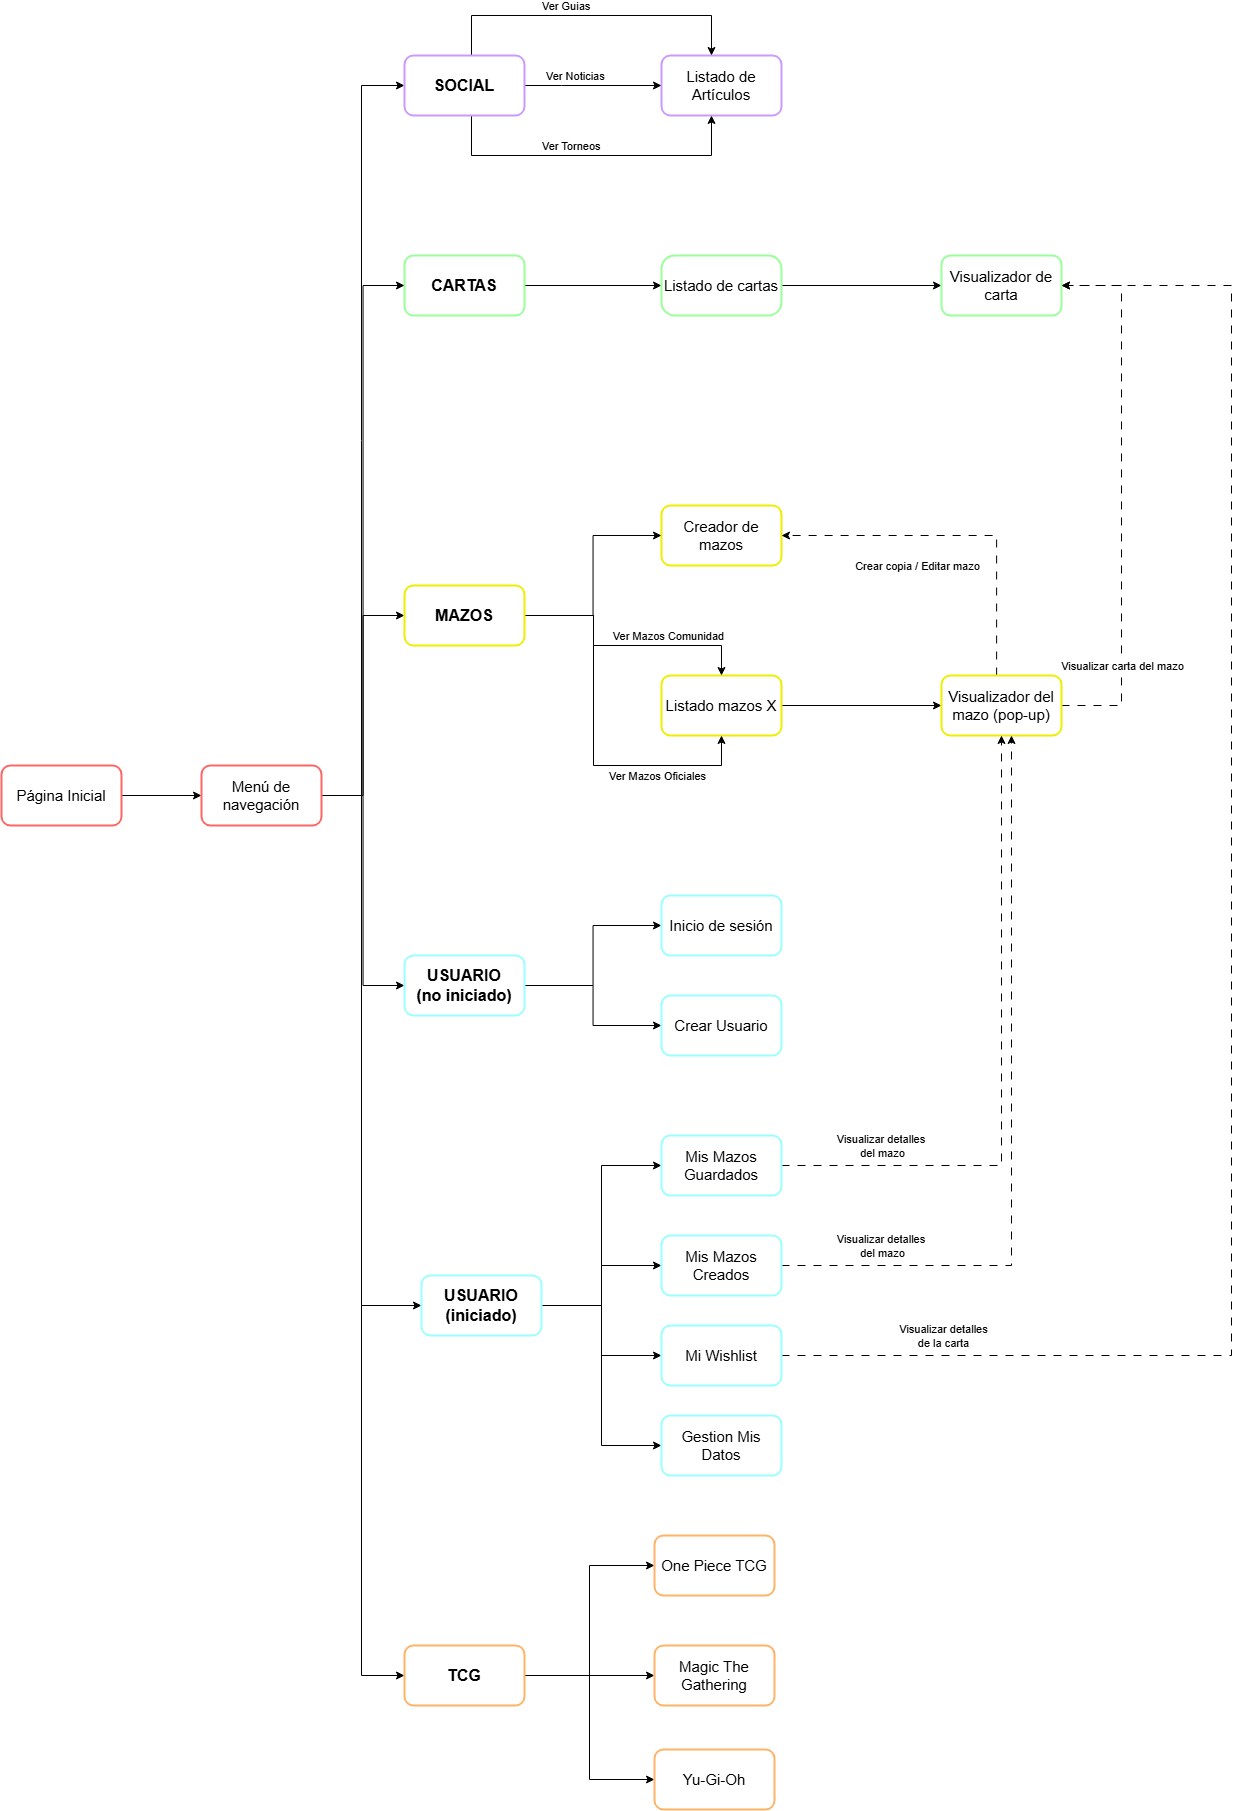
\includegraphics[width=1\textwidth]{Recursos/Mapa Card Partner v3.png}
		\caption{Estructura jerárquica y mapa del sitio web de Card Partner.}
		\label{fig:mapa_sitio}
	\end{figure}
	
	\subsection{Flujos de navegación}
		\subsubsection{Consulta de mazos}
			El usuario quiere consultar los mazos del META del TCG de One Piece.\\
			El usuario accede a la web a la \textbf{Página Inicial}, desde allí en el \textbf{Menú de navegación} se encontrará con varios desplegables, entre ellos \textbf{MAZOS} que mostrará varias opciones y una de las opciones será \textbf{Listado mazos META}.
			\begin{center}
				\textbf{Página Inicial} $\rightarrow$ \textbf{MAZOS} $\rightarrow$ \textbf{Listado mazos META}
			\end{center}
		\subsubsection{Consultar noticias}
		El usuario quiere informarse sobre las últimas novedades, expansiones o anuncios del juego.\\
		El usuario accede a la \textbf{Página Inicial}. En el \textbf{Menú de navegación}, accede desde el apartado \textbf{SOCIAL}, y al pulsar sobre la opción \textbf{Ver Noticias} el sistema le redirige al \textbf{Listado de Artículos(Noticias)}.
		\begin{center}
			\textbf{Página Inicial} $\rightarrow$ \textbf{SOCIAL} $\rightarrow$ \textbf{Ver Noticias} $\rightarrow$ \textbf{Listado de Artículos}
		\end{center}
			
		\subsubsection{Consulta de cartas}
		El usuario necesita buscar los detalles, el efecto o el precio de mercado actual de una carta específica.\\
		El usuario entra en la \textbf{Página Inicial} y selecciona \textbf{CARTAS} en el \textbf{Menú de navegación}. Esto le lleva al catálogo general, donde tras aplicar filtros y buscar la carta deseada, hace clic sobre ella para abrir una vista detallada con toda su información.
		\begin{center}
			\textbf{Página Inicial} $\rightarrow$ \textbf{CARTAS} $\rightarrow$ \textbf{Listado de cartas} $\rightarrow$ \textbf{Visualizador de carta}
		\end{center}
		
		\subsubsection{Consultar detalle de una carta desde un mazo}
		Mientras el usuario estudia la composición de una baraja, se encuentra con una carta que no conoce y necesita ver sus atributos, efectos o precio de mercado.\\
		El usuario se encuentra visualizando un mazo desde el \textbf{Visualizador del mazo}. Al hacer clic sobre una carta específica del listado, la web le redirigirá directamente la carta específica mediante el \textbf{Visualizador de carta}, sin tener que buscarla manualmente en el catálogo.
		\begin{center}
			\textbf{Página Inicial} $\rightarrow$ \textbf{MAZOS} $\rightarrow$ \textbf{Listado mazos X} $\rightarrow$ \textbf{Visualizador del mazo} $\rightarrow$ \textbf{Visualizador de carta}
		\end{center}
		
		\subsubsection{Navegación por guías de juego}
		Un usuario principiante quiere aprender las mecánicas básicas para iniciarse en el TCG de One Piece.\\
		El usuario accede a la \textbf{Página Inicial} y despliega el \textbf{Menú de navegación}. Se dirige a la sección \textbf{SOCIAL} y selecciona la opción \textbf{Ver Guías}. El sistema renderiza el \textbf{Listado de Artículos} filtrando la base de datos para mostrar únicamente el contenido de aprendizaje, permitiendo al usuario acceder a las explicaciones.
		\begin{center}
			\textbf{Página Inicial} $\rightarrow$ \textbf{SOCIAL} $\rightarrow$ \textbf{Ver Guías} $\rightarrow$ \textbf{Listado de Artículos}
		\end{center}
    
		% Apartado MAPA WEB:\\
		
		% El mapa no incluye explícitamente una página de perfil propio (gestión de datos del usuario, cambio de contraseña) como nodo diferenciado; aparece como "Gestión Mi Cuenta" pero sin desarrollar qué contiene.\\
		
		% La sección TCG aparece en el mapa como una opción de ampliación futura, pero ya está implementada en las páginas estáticas. Podría haberse integrado mejor en el mapa como sección funcional actual.\\
	
	
	\section{Base de datos}
		Para la base de datos se ha elegido usar MariaDB a través de XAMPP para facilitar el trabajo de gestión y diseño, ya que permite usar phpMyAdmin desde navegadores web y gestionar la base de datos de manera visual y exportar o importar los scripts de creación e inserción de datos,  además de otras herramientas útiles (como el meter csv).
		\subsection{Cambios del Modelo de Dominio a Entidad-Relacion}
			Para traducir el modelo de dominio realizado en la práctica 2 al modelo entidad-relacion de la base de datos, se han realizado los siguientes cambios:
			\begin{itemize}
				\item \textbf{Usuario}: \\
					Se ha traducido la relación de \textit{Usuario} como clase padre de \textit{Jugador} y \textit{Admin} a una sola tabla \texttt{Usuario} y un atributo ROL que especifique que tipo de usuario es.
				\item \textbf{Mazo}: \\
					Al igual que con \textit{Usuario}, la clase \textit{Mazo} se ha traducido a una única tabla \texttt{Mazo} y un atributo ES\_OFICIAL para hacer la distinción.
				\item \textbf{Relaciones *:*}: \\
					Las relaciones muchos a muchos entre \textit{Jugador}-\textbf{GUARDA}-\textit{Mazo}, \textit{Mazo}-\textbf{CONTIENE}-\textit{Carta} y \textit{Jugador}-\textbf{VALORA}-\textit{Mazo} se han traducido como las clases intermedias \texttt{GUARDA\_MAZO}, \texttt{CONTIENE\_CARTA} y \texttt{VALORACION} respectivamente.
				
			\end{itemize}
			
			\begin{figure}[H]
				\centering
				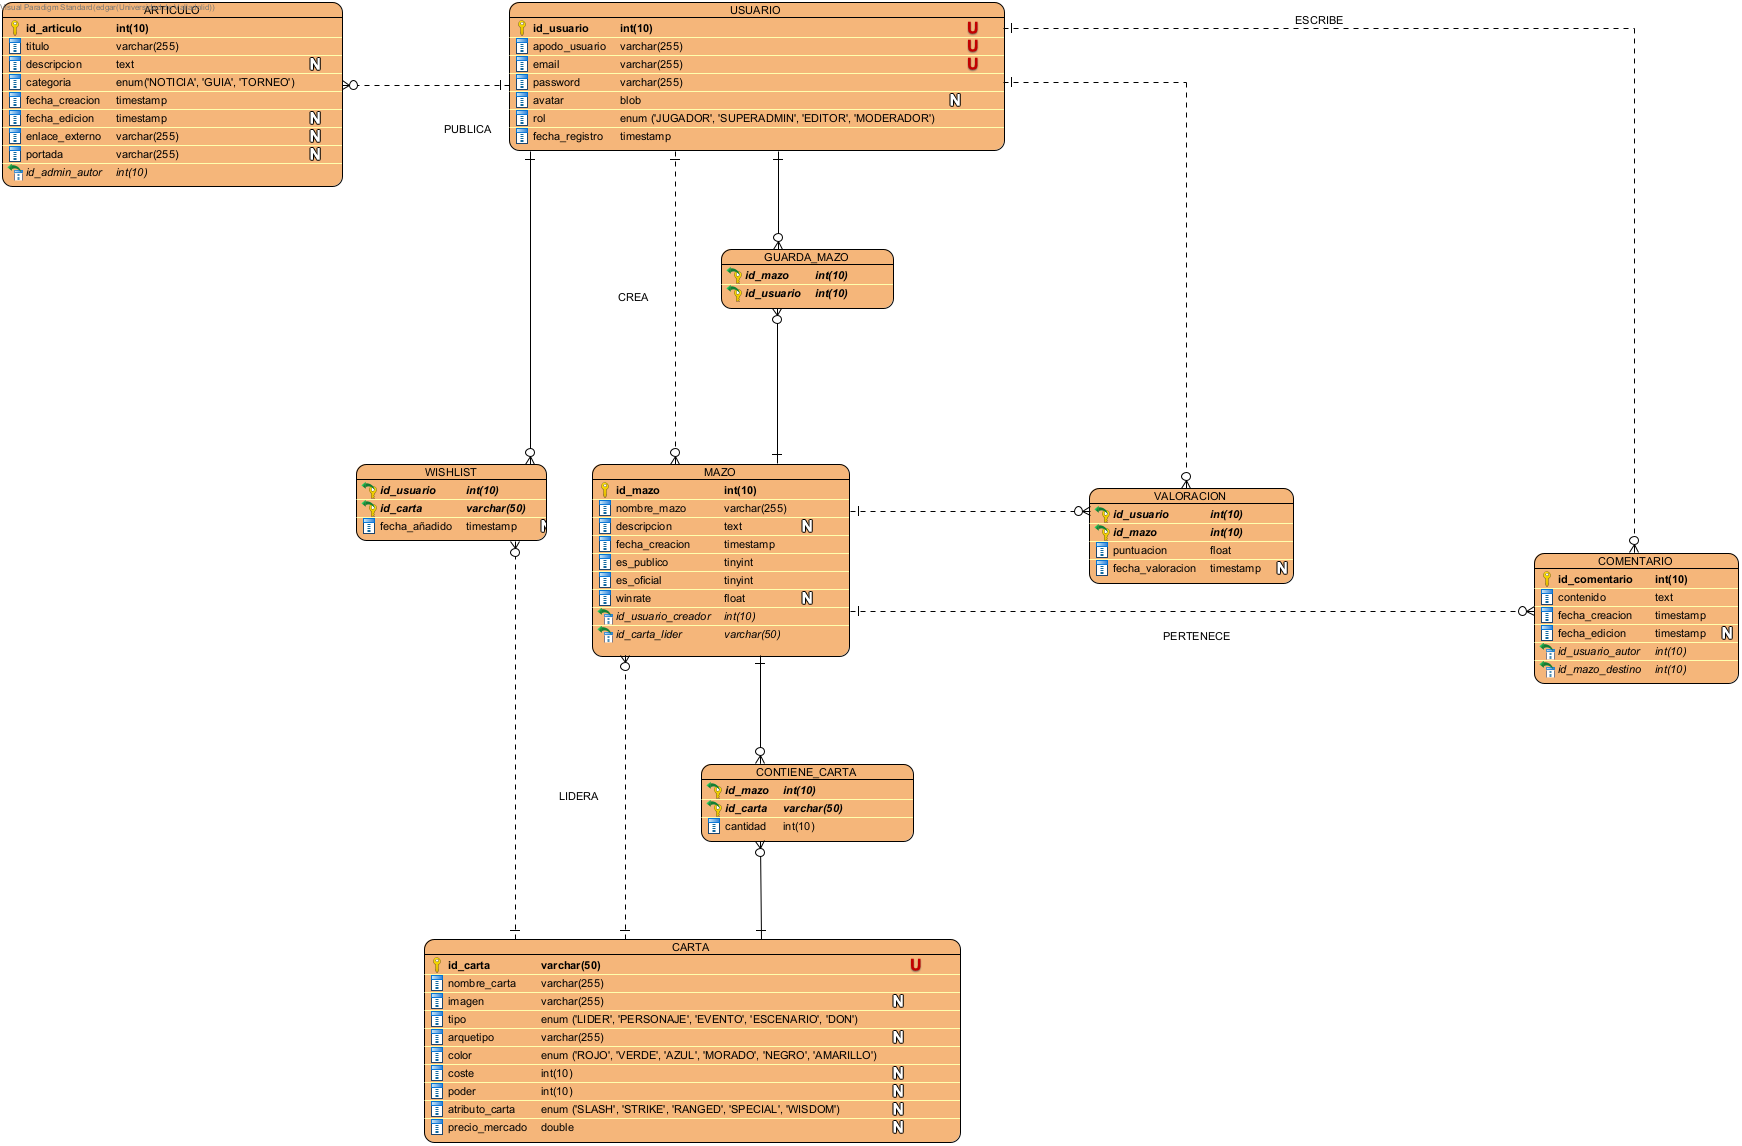
\includegraphics[width=1\textwidth]{Recursos/CardPartner_DBv2.png}
				\caption{Entidad-Relacion de la base de datos}
				\label{fig:mapa_sitio}
			\end{figure}
			
			
			\subsection{Estructura de la Base de Datos}
			
			La base de datos \texttt{cardpartner\_db} está diseñada bajo un modelo relacional orientado a la gestión de una comunidad de juegos de cartas coleccionables (TCG). Su arquitectura se divide en cuatro pilares fundamentales:
			
			\subsection{Componentes Principales}
			
			\begin{itemize}
				\item \textbf{Gestión de Usuarios y Roles:} La entidad \texttt{USUARIO} centraliza el acceso y la seguridad. Mediante un sistema de roles (\textit{Jugador, Editor, Moderador, Superadmin}), se definen los niveles de interacción con la plataforma.
				\item \textbf{Catálogo de Cartas y Mazos:} 
				\begin{itemize}
					\item \texttt{CARTA}: Actúa como el diccionario técnico del juego, almacenando atributos estáticos como coste, poder, color y tipo.
					\item \texttt{MAZO}: Representa la agrupación lógica de cartas creada por un usuario, vinculada obligatoriamente a una carta líder.
				\end{itemize}
				\item \textbf{Módulo de Comunidad:} La interacción social se articula a través de las tablas \texttt{VALORACION}, \texttt{COMENTARIO} y \texttt{GUARDA\_MAZO}, permitiendo la retroalimentación y la creación de bibliotecas personales.
				\item \textbf{Sistema de Contenidos:} La entidad \texttt{ARTICULO} permite a los administradores gestionar noticias, guías y torneos, manteniendo la plataforma actualizada.
			\end{itemize}
			
			\subsubsection{Resumen de Relaciones y Cardinalidad}
			
			En esta sección comentamos las cardinalidades y relaciones en forma de tabla con una pequeña explicación de lo que significan para poder complementar el E/R.
			
			\begin{table}[H]
				\centering
				
				\begin{tabularx}{\textwidth}{l l X}
					\toprule
					\textbf{Relación} & \textbf{Tipo} & \textbf{Descripción} \\
					\midrule
					Usuario $\rightarrow$ Mazo & 1:N & Un usuario es autor de múltiples mazos. \\
					Mazo $\leftrightarrow$ Carta & N:M & Relación gestionada por \texttt{CONTIENE\_CARTA} con cantidades. \\
					Usuario $\leftrightarrow$ Mazo & N:M & Biblioteca personal y favoritos (\texttt{GUARDA\_MAZO}). \\
					Usuario $\rightarrow$ Articulo & 1:N & Relación de autoría para perfiles administrativos. \\
					\bottomrule
				\end{tabularx}
				\caption{Resumen de la Arquitectura de Datos} 
			\end{table}
			
			\subsection{Inserción de los datos en la BBDD en Apache NetBeans}
			
				\begin{figure}[H]
					\centering
					% Primera imagen
					\begin{minipage}{0.45\textwidth}
						\centering
						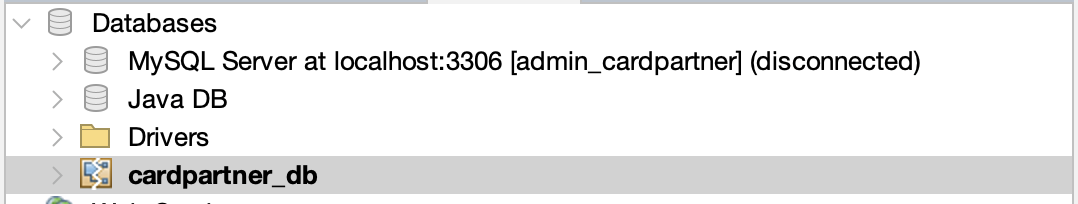
\includegraphics[width=\textwidth]{Recursos/BBDD_CONEXION.png}
						\caption{Hemos configurado la conexión en el Apache NetBeans con una base de datos MariaDB en el localhost con su puerto por defecto.}
						\label{fig:img1}
					\end{minipage}
					\hfill % Espacio elástico para separar las imágenes
					% Segunda imagen
					\begin{minipage}{0.45\textwidth}
						\centering
						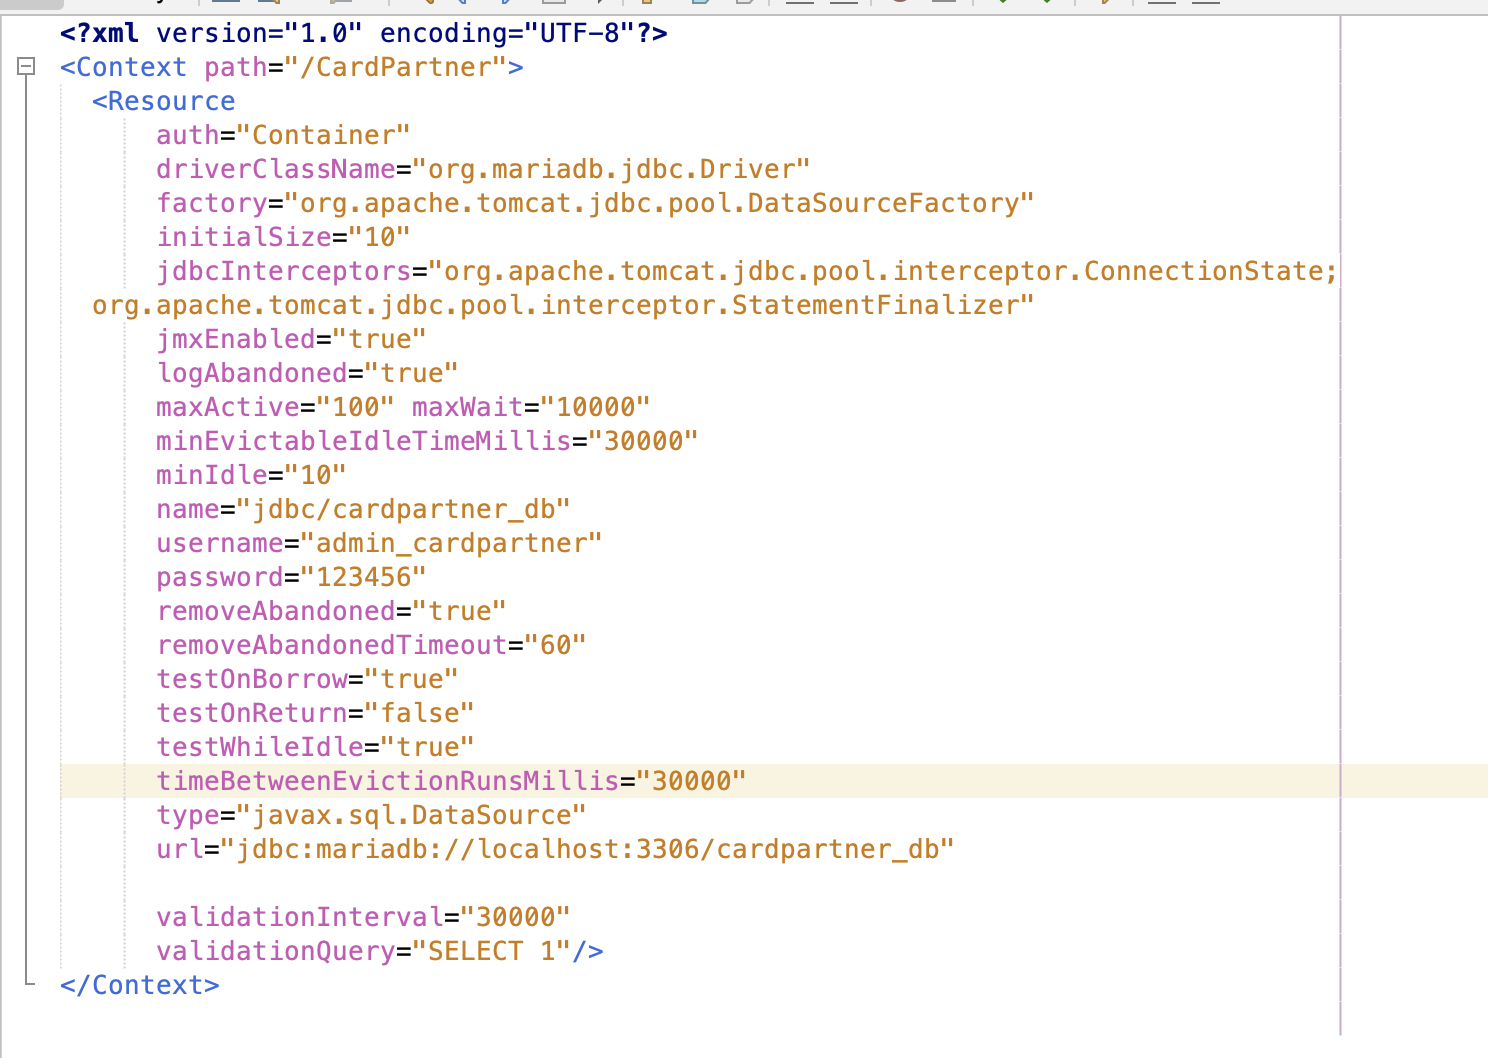
\includegraphics[width=\textwidth]{Recursos/XMLBBDD.png}
						\caption{Modificamos el \textit{context.xml} del editor para poder establecer la conexión permanente con la bbdd en nuestro proyecto.}
						\label{fig:img2}
					\end{minipage}
				\end{figure}
				
				
				El problema que hemos tenido es que al establecer la conexión y hacer un \textit{push} al repositorio, Edgar, no tenía la conexión establecedia en el Apache, tras una tutoría con el profesor del laboratio, nos ha explicado que como no contamos con un servidor donde alojar la base de datos, realmente no había ninguna manera de hacer esta conexión persistente, por lo que tomamos la decisión de hacer unos scripts, que hagan la creación de la base de datos en local más simple, facilitando así su posterior conexión con el editor de código.\\ 
				
					\begin{figure}[H]
					\centering
					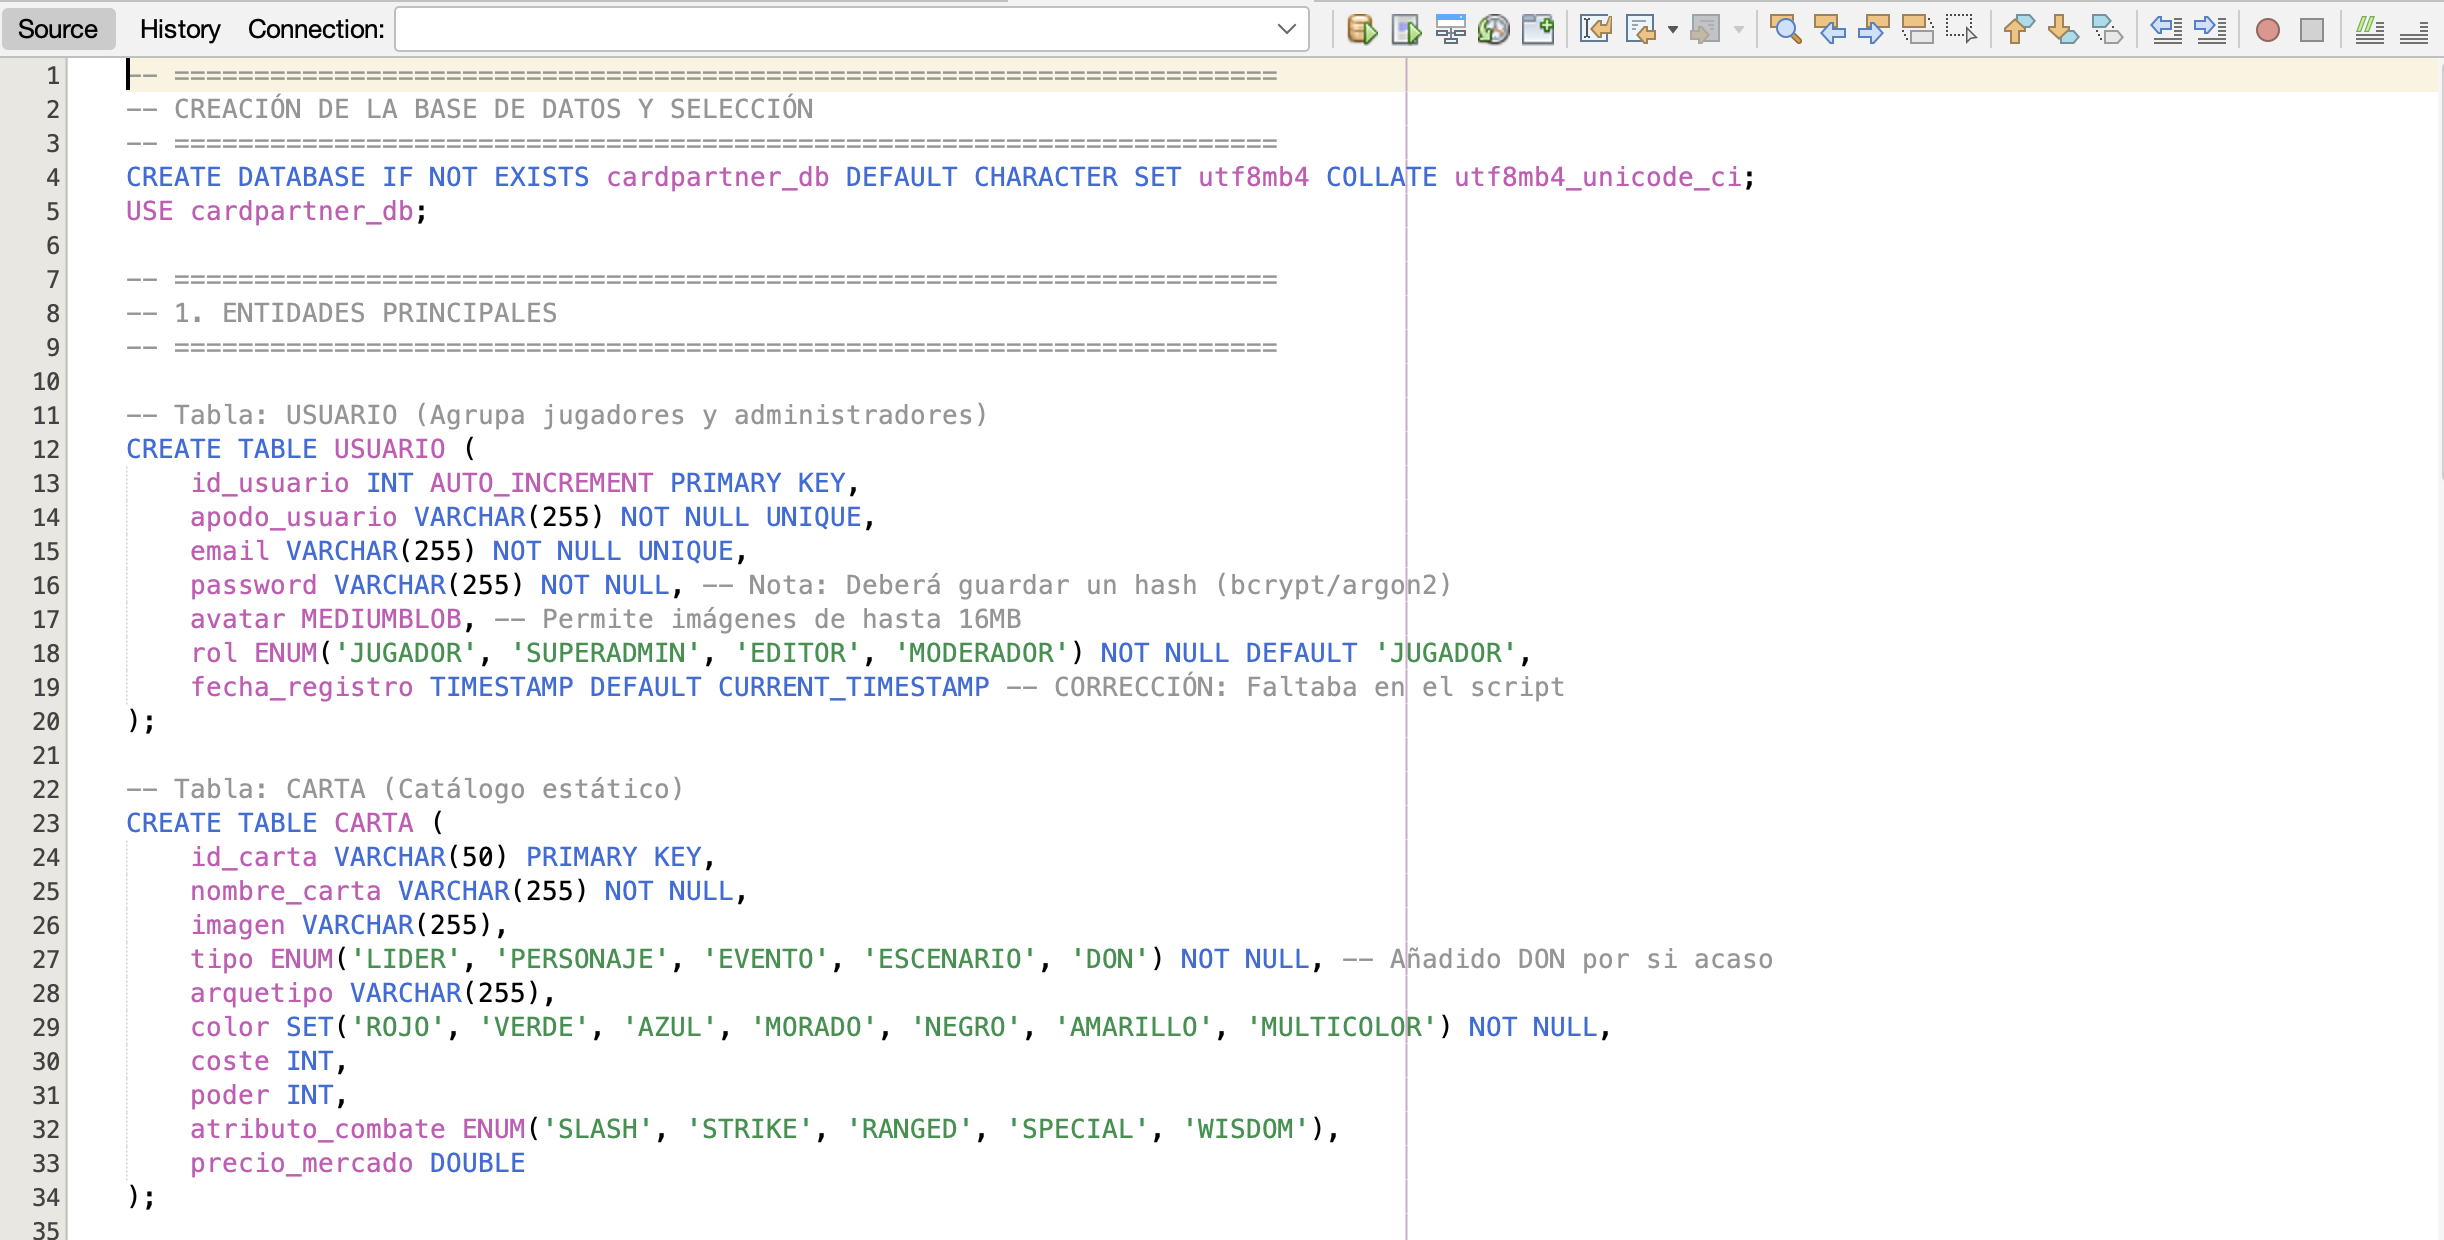
\includegraphics[width=1\textwidth]{Recursos/creacionBBDD.png}
					\caption{Además, para que todos tengamos las mismas tablas, hemos incluido el script \textit{CreacionDBv2.sql} para que genere automáticamente las tablas (por motivos de brevedad no hemos incluido todo el script ya que se puede consultar en \textit{Files/sql} dentro del apache)}.
					\label{fig:creacion}
				\end{figure}
				
				
			\subsubsection{Inserción de los datos en las tablas}
				Para esta parte, debido al poco tiempo que hemos tenido para desarrollar la práctica por el calendario tan ajustado de entregas del curso, hemos decidido tener 2 scripts .sql para poblar la base de datos, los cuales se encuentran en \textit{FIles/sql} dentro del Apache NetBeans.\\

				Adicionalmente, para que fuese más cómodo y por un tema de estructura y revisión del código, hay una carpeta en nuestro repositorio de git (por ende en el zip en el que hemos entregado la práctica) llamado \textit{DataBase} donde se encuentra el E/R, los scripts de creación de las tablas y  los encargados de poblararla, así como los JSONs de los que hemos partidos para las cartas.\\
				
				Queda pendiente para la siguiente entrega, modificar los DAOS y DTOs para que al emplear la librería java \hyperlink{https://mvnrepository.com/artifact/com.google.code.gson/gson/2.10.1}{GSON}, se encargue atuomáticamente de llenar la base de datos de cartas en función de un JSON, pero por motivos de coplejidad no hemos podido realizar dicha tarea para la actual entrega.\\

			 	\begin{figure}[htbp]
				 	\centering
				 	% Primera imagen
				 	\begin{minipage}{0.45\textwidth}
				 		\centering
				 		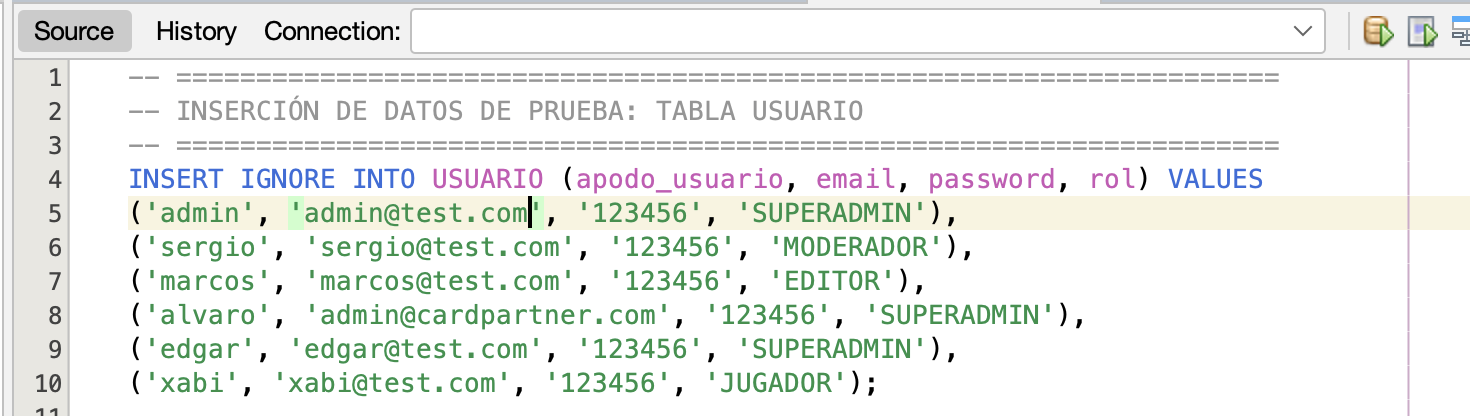
\includegraphics[width=\textwidth]{Recursos/InsertUsuario.png}
				 		\caption{Hacemos un insert, con la peculiaridad de que usamos el modificador de sentencia \textit{IGNORE} para que en caso de añadir más cartas, si encuentra la \textit{primarykey} en la bbdd pasa de él.}
				 		\label{fig:imgInsert}
				 	\end{minipage}
				 	\hfill % Espacio elástico para separar las imágenes
				 	% Segunda imagen
				 	\begin{minipage}{0.45\textwidth}
				 		\centering
				 		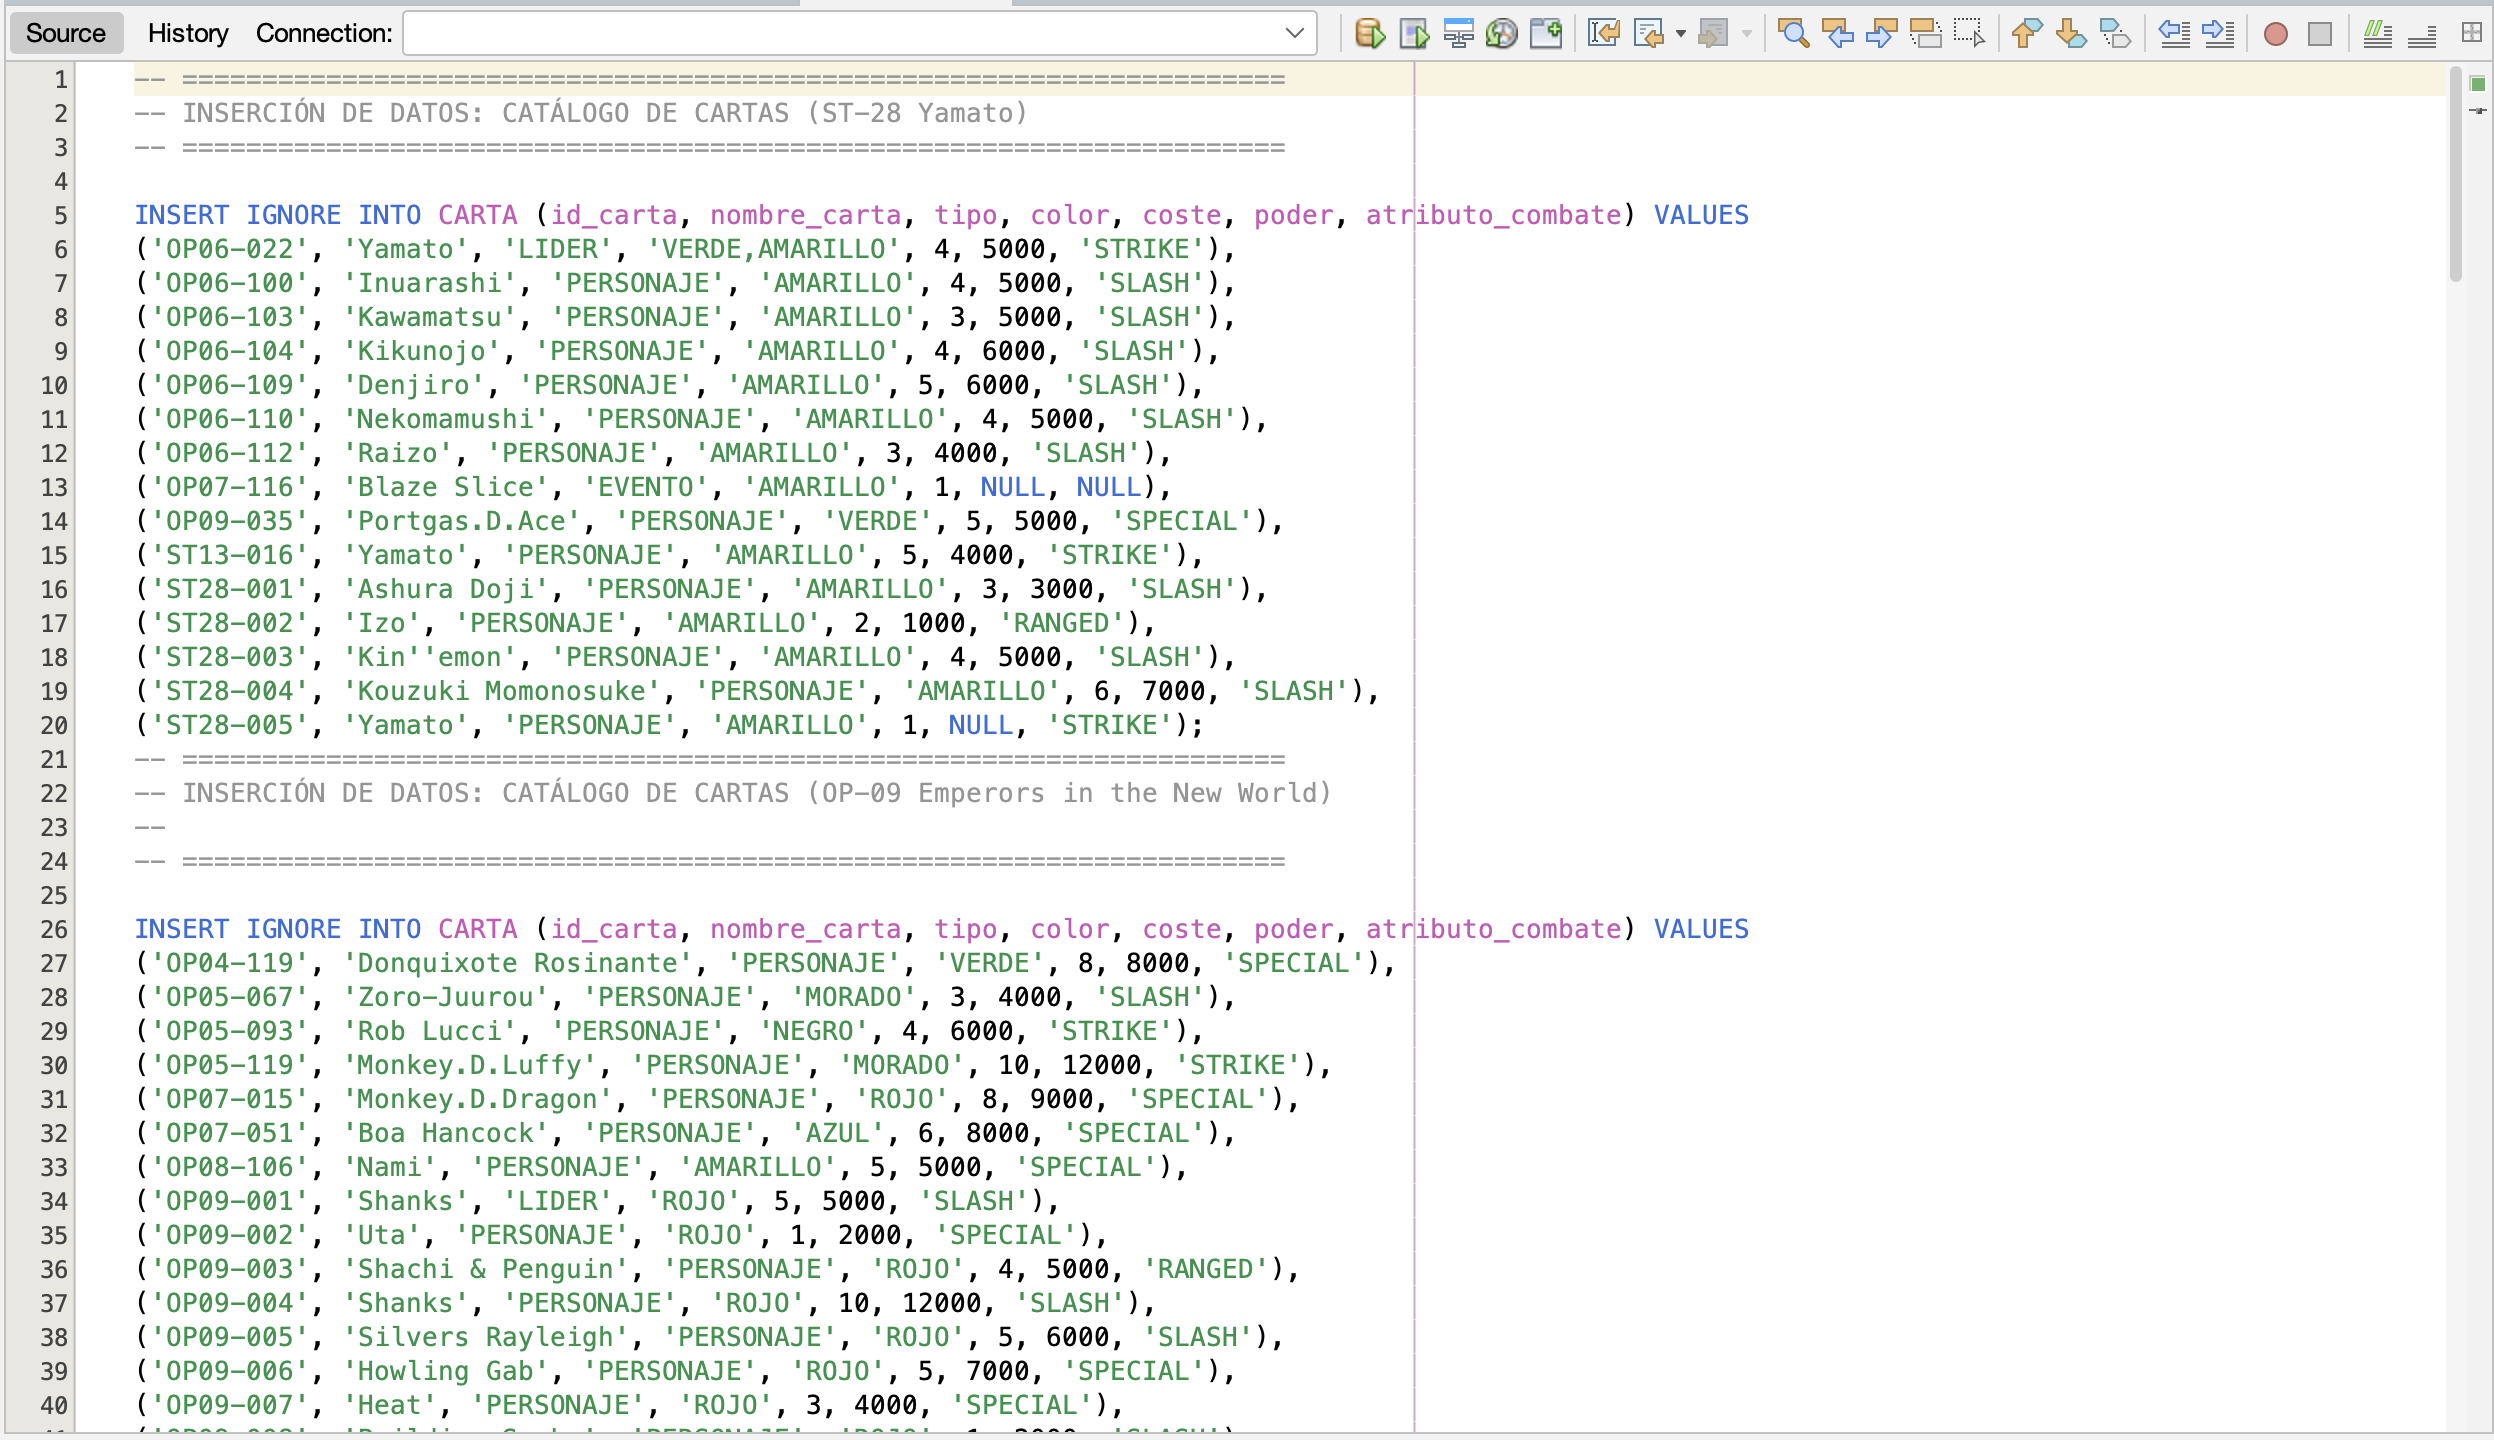
\includegraphics[width=\textwidth]{Recursos/InsertCartas.png}
				 		\caption{Script de población de la bbdd de cartas donde hemos insertado todas las cartas desde OP9 a OP12 además de un \textit{starter deck} para que los compañeros de front tengan cartas de sobra. Al igual que en el insert anterior empleamos el modificador de sentencia \textit{IGNORE}.}
				 		\label{fig:insertarCartas}
				 	\end{minipage}
				 \end{figure}
				 
			\subsection{Consideraciones Técnicas}
			El diseño implementa integridad referencial mediante el uso de \texttt{ON DELETE CASCADE}, asegurando que la eliminación de una entidad principal (como un usuario) limpie automáticamente sus datos dependientes. Además, se han optimizado los tipos de datos utilizando \texttt{ENUM} para categorías fijas y \texttt{SET} para la gestión de colores múltiples en las cartas.
			\begin{itemize}
				\item \textbf{Gestión de Tiempos (\textit{Timestamps} vs \textit{Date}):} Se ha optado por el uso de \texttt{TIMESTAMP} en lugar de \texttt{DATE} para columnas como \texttt{fecha\_registro} y \texttt{fecha\_edicion}. Esto permite una precisión de segundos y, sobre todo, aprovecha la funcionalidad \texttt{DEFAULT CURRENT\_TIMESTAMP} y \texttt{ON UPDATE CURRENT\_TIMESTAMP}, automatizando el seguimiento de cambios sin necesidad de lógica adicional en el backend.
				
				\item \textbf{Uso de Tipos Enumerados (\textit{ENUM} y \textit{SET}):} 
				\begin{itemize}
					\item Se emplea \texttt{ENUM} para roles y categorías de artículos para restringir los valores a un conjunto cerrado, mejorando el rendimiento y evitando datos inconsistentes.
					\item Se utiliza \texttt{SET} para el atributo \texttt{color} en las cartas, ya que permite que una sola carta pertenezca a múltiples categorías simultáneamente (cartas multicolores) de forma eficiente a nivel de bits.
				\end{itemize}
				
				\item \textbf{Política de Nulidad (\textit{Nullable}):} La mayoría de los campos críticos se han definido como \texttt{NOT NULL} para garantizar la calidad del dato. Los campos \texttt{NULL} (como \texttt{enlace\_externo} o \texttt{portada}) se reservan exclusivamente para información opcional o metadatos que no interrumpen el flujo principal de la aplicación.
				
				\item \textbf{Almacenamiento de Binarios:} Para los avatares de usuario, se ha seleccionado \texttt{MEDIUMBLOB}. Aunque el estándar suele ser guardar rutas de archivos, incluir el binario (hasta 16MB) facilita la portabilidad inicial del proyecto y simplifica la gestión de copias de seguridad de la base de datos completa.
				
				\item \textbf{Claves Primarias y Foráneas:} Se utilizan \texttt{INT AUTO\_INCREMENT} para entidades dinámicas (usuarios, mazos) para agilizar las búsquedas, mientras que las cartas utilizan un \texttt{VARCHAR(50)} como ID, permitiendo usar códigos alfanuméricos oficiales (ej: \"OP01-001\") que facilitan la integración con APIs externas.
			\end{itemize}
	
	\section{Descripción de la funcionalidad implementada y justificación de la elección}
		En Card Partner, hemos implementado un conjunto de funcionalidades que reflejan tanto los requisitos identificados en las entregas anteriores como las necesidades reales de los jugadores de TCG. La elección de cada módulo se ha realizado teniendo en cuenta la experiencia de usuario, la coherencia con el modelo de dominio y la facilidad de mantenimiento del sistema.

		\subsection{Gestión de usuarios y perfil}
			Hemos desarrollado un sistema de usuarios que distingue claramente entre visitantes, jugadores registrados y administradores. Los visitantes pueden consultar contenido público, como cartas, noticias, guías, torneos y mazos públicos, sin necesidad de registrarse. Los jugadores registrados disponen de un perfil completo que les permite gestionar sus datos, cambiar la contraseña, crear y guardar mazos, comentar y valorar los mazos de la comunidad. Los administradores tienen privilegios para publicar mazos oficiales y artículos, así como mantener el contenido de la web actualizado.\\

			Para esta funcionalidad, hemos decidido centralizar toda la gestión de datos en la sección de \textbf{Perfil}, permitiendo a los usuarios acceder a sus activos y configuraciones desde un único panel. Esta elección garantiza que la administración de la información sea intuitiva y accesible, evitando dispersión en múltiples páginas.

		\subsection{Gestión y creación de mazos}
			El constructor de mazos (Deckbuilder) ha sido implementado con ventanas emergentes modales que permiten seleccionar cartas, asignar la carta líder y configurar la composición completa de un mazo. Hemos decidido incluir tanto mazos de la comunidad como mazos oficiales/meta, diferenciándolos mediante el atributo \texttt{es\_publico} o \texttt{winrate}. Esto permite que los jugadores puedan crear, guardar y consultar mazos de manera flexible, mientras que los mazos oficiales permanecen verificados y orientados a la escena competitiva.\\

			Además, se han creado vistas de detalle de mazo que muestran el precio total, estadísticas y cartas contenidas, facilitando la toma de decisiones al jugador y mejorando la experiencia de navegación.

		\subsection{Catálogo de cartas y filtros}
			Hemos implementado un listado completo de todas cartas disponibles, con filtros avanzados por nombre, color, tipo, coste y rareza. Cada carta muestra sus atributos principales y su precio de mercado. La decisión de incluir estos filtros se basa en la necesidad de los jugadores de localizar rápidamente cartas específicas y planificar la construcción de sus mazos de forma eficiente.

		\subsection{Comunidad e interacción}
			Se ha integrado un sistema de comentarios y valoraciones en cada mazo. Los jugadores pueden publicar sus opiniones, sugerir cambios y puntuar mazos creados por otros usuarios. Esta funcionalidad se conecta directamente con la gestión de usuarios, asegurando que solo los jugadores registrados puedan participar, mientras que los visitantes pueden consultar el contenido publicado.

		\subsection{Contenido editorial}
			Hemos desarrollado secciones de noticias, guías y torneos, gestionadas por los administradores. Esta elección permite mantener la plataforma actualizada, ofreciendo información relevante y útil para jugadores principiantes y experimentados, y consolidando a \textbf{Card Partner} como un punto de referencia dentro de la comunidad TCG.

		\subsection{Sección TCG}
			Aunque inicialmente se había considerado como ampliación futura, hemos decidido integrar la sección TCG de manera completa en esta parte. Esta sección proporciona reglas, mecánicas y recursos adicionales del TCG de One Piece, ofreciendo una base educativa y de referencia para los nuevos jugadores, y permitiendo a los jugadores avanzados acceder a información sobre cartas y mazos oficiales.

		\subsection{Justificación de la elección}
			Hemos optado por implementar estas funcionalidades priorizando:

			\begin{itemize}
				\item Centralización de información y herramientas, evitando que los jugadores tengan que usar múltiples webs externas.
				\item Claridad y facilidad de uso, con un panel de perfil único y vistas modales en el constructor de mazos.
				\item Escalabilidad, permitiendo agregar nuevas cartas, mazos o secciones sin necesidad de reescribir la estructura base del sistema.
				\item Interacción social, fomentando la participación de la comunidad mediante comentarios y valoraciones.
				\item Coherencia con el modelo de dominio y la base de datos, asegurando que la estructura de información sea consistente y fácil de mantener.
			\end{itemize}

			Con estas decisiones, \textbf{Card Partner} ofrece una plataforma funcional, intuitiva y completa, que cubre las necesidades más importantes de los jugadores de TCG y justifica las elecciones de diseño realizadas en el desarrollo del sistema.
				
	\section{Instrucciones de ejecución del código}
			\begin{itemize}
				\item Ejecutar el script de \textit{setup\_db} (que se encuentran en \textit{CardPartner/sql/} o en el directorio raiz de SSW si se mira desde el repositorio de GitHub)
				\item Realizar la conexión con la bbdd en el Apache NetBeans
			\end{itemize}
			\begin{figure}[H]
				\centering
				% Primera imagen
				\begin{subfigure}[b]{0.3\textwidth}
					\centering
					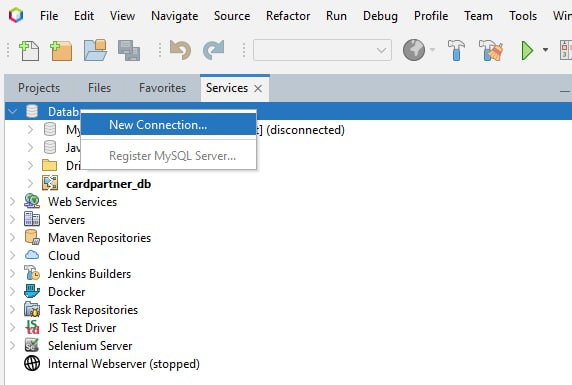
\includegraphics[width=\textwidth]{Recursos/Services.jpg}
					\caption{Vamos al menú de \textit{services} del editor}
				\end{subfigure}
				\hfill % Espaciado horizontal elástico
				% Segunda imagen
				\begin{subfigure}[b]{0.3\textwidth}
					\centering
					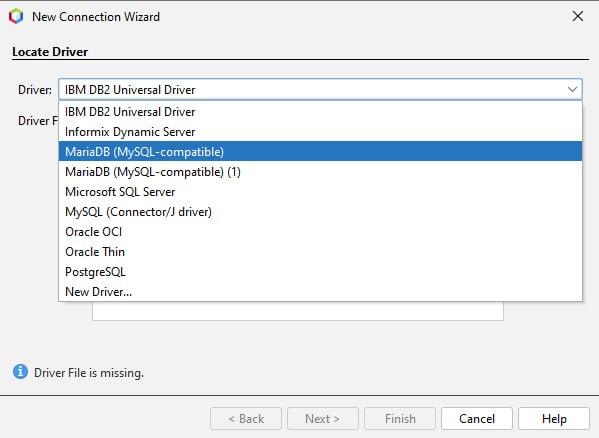
\includegraphics[width=\textwidth]{Recursos/DriverMDB.jpg}
					\caption{En el menú desplegable seleccionamos nuestra base de datos y buscamos el driver que se encuentra en la carpeta lib de nuestro proyecto}
				\end{subfigure}
				\hfill % Espaciado horizontal elástico
				% Tercera imagen
				\begin{subfigure}[b]{0.3\textwidth}
					\centering
					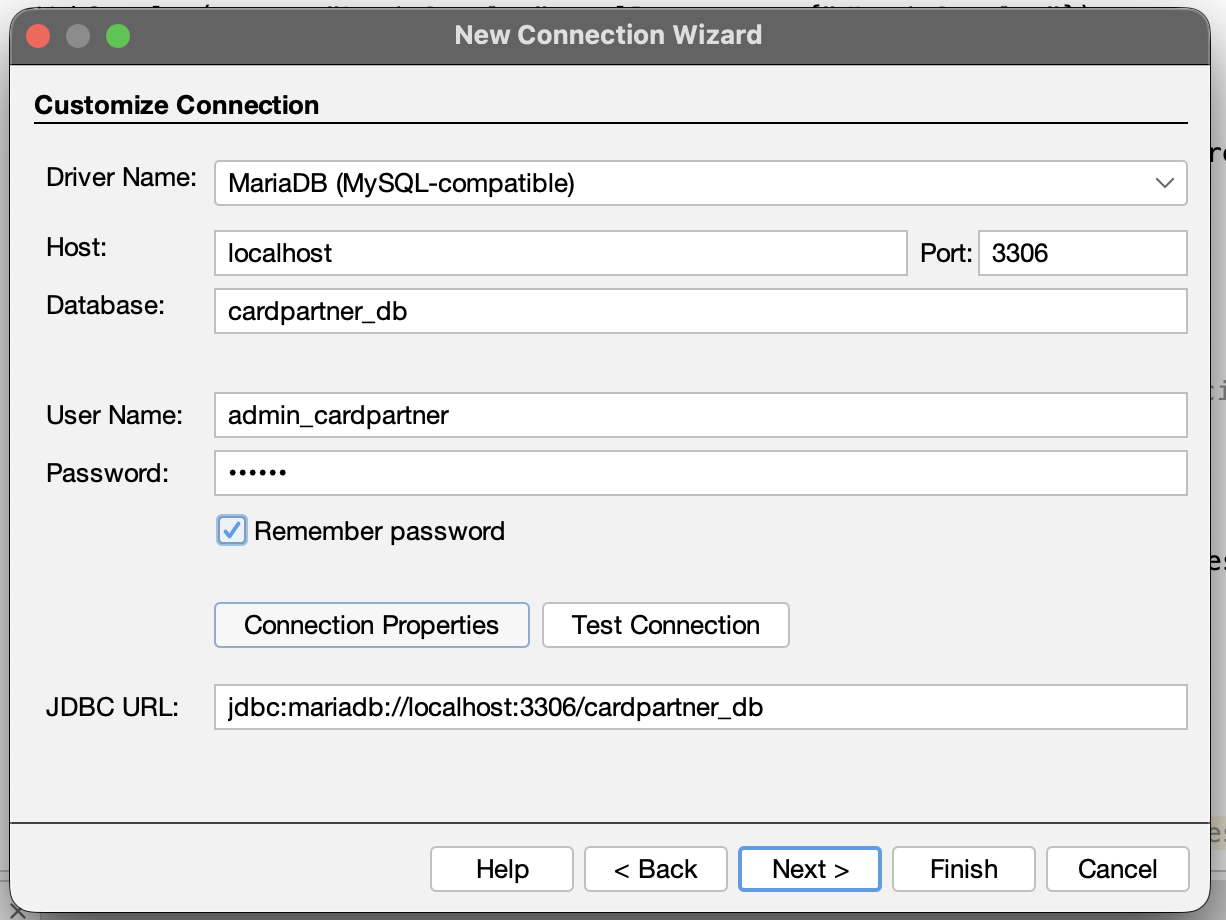
\includegraphics[width=\textwidth]{Recursos/ConexionBBDD.png}
					\caption{Introducimos el nombre de nuestra base de datos (cardpartner\_db) con su usuario (admin\_cardpartner) y la contraseña (123456)}
					
				\end{subfigure}
				
			\end{figure}
			\begin{itemize}
				\item Vamos al menú de Files del editor
				\item Dentro de este menú, buscamos la carpeta que se llame sql 
				\item Ejecutamos los scripts en orden para tener toda la información necesaria en nuestra base de datos.
				\item Ejecutamos la aplicación.
			\end{itemize}
			
			\subsection{Usuarios para login}
				Para la funcionalidad de inicio de sesion, se han creado los siguientes usuarios en la base de datos:
				
			\begin{table}[H]
				\centering
				
				\vspace{0.3cm} % Espacio entre caption y tabla
				\begin{tabular}{c c c} 
					\toprule
					\textbf{Apodo} & \textbf{Email} & \textbf{Password} \\
					\midrule
					admin  & admin@test.com        & 123456 \\
					sergio & sergio@test.com       & 123456 \\
					marcos & marcos@test.com       & 123456 \\
					alvaro & admin@cardpartner.com & 123456 \\
					edgar  & edgar@test.com        & 123456 \\
					xabi   & xabi@test.com         & 123456 \\
					\bottomrule
				\end{tabular}
				\caption{Credenciales de usuarios para pruebas de sistema}
				\label{tab:usuarios_prueba}
			\end{table}
	
	\section{Declaración de Uso de Inteligencia Artificial}
		Para esta segunda entrega, se ha usado la IA Gemini como herramienta para dudas y mejoras del archivo LaTeX, revisión de los contenidos y evaluación de los mismos y diseño iterativo para mejorar lo ya realizado.\\
		Además, se ha usado \href{https://gemini.google.com/share/7a923a0bfae8}{Gemini} para la generación del logo del proyecto.\\
		\textbf{Ejemplos de prompts realizados:}
		\begin{itemize}
			\item 'Cómo funciona un servlet en java'
			\item 'Que son los DAOs, DTOs y Servlets en java y como es el flujo de trabajo entre ellos'
			\item 'Como hacer una conexión de MariaDB en ApacheNetBeans'
			\item 'Haciendo push, a mis compañeros no les aparece la bbdd ¿es normal?'
			\item 'Cómo puedo automatizar la instalación y creación de una bbdd con MariaDB'
			\item 'Me puedes revisar los \textit{scripts} de creación de la base de datos'
			\item 'Traduceme este \textit{script} de creación de bbdd para Windows en un .bat'
			\item 'Cómo puedo testear que la base de datos se ha rellenado de manera correcta con los \textit{scrpts} sql'
			\item 'Cómo me puedo saltar la política CORS para hacer peticiones a la web de bandai nanco sobre cartas del tcg de One Piece'
			\item 'Cómo puedo cambiar la numeración de una página para sean botones y mejorar la navegabilidad por una lista de cartas'
	        \item 'Ayudame a mejorar el botón de filtros de la vista cartas'
	        \item '¿Cómo puedo añadir un mensaje de aviso que indique que no se puede acceder a esta vista sin estar loggeado?'
	        \item 'No logro que se apliquen los filtros en las cartas, ¿puedes echarme una mano?'
		\end{itemize}
	
	%\begin{itemize}
	%   \item Herramientas utilizadas: hay que especificar qué herramientas de IA se han utilizado.
	%  \item Propósito del uso: explicar cómo se ha utilizado cada herramienta.
	% \item Alcance del uso: indicar en qué partes específicas del trabajo se ha recibido asistencia de una herramienta de IA.
	%\item Prompts utilizados: incluir los prompts, preguntas o instrucciones exactas que se han
	%introducido en la herramienta de IA.
	%\end{itemize}
	
\end{document}